\documentclass[twoside]{book}

% Packages required by doxygen
\usepackage{fixltx2e}
\usepackage{calc}
\usepackage{doxygen}
\usepackage[export]{adjustbox} % also loads graphicx
\usepackage{graphicx}
\usepackage[utf8]{inputenc}
\usepackage{makeidx}
\usepackage{multicol}
\usepackage{multirow}
\PassOptionsToPackage{warn}{textcomp}
\usepackage{textcomp}
\usepackage[nointegrals]{wasysym}
\usepackage[table]{xcolor}

% NLS support packages
\usepackage{polski}
\usepackage[T1]{fontenc}

% Font selection
\usepackage[T1]{fontenc}
\usepackage[scaled=.90]{helvet}
\usepackage{courier}
\usepackage{amssymb}
\usepackage{sectsty}
\renewcommand{\familydefault}{\sfdefault}
\allsectionsfont{%
  \fontseries{bc}\selectfont%
  \color{darkgray}%
}
\renewcommand{\DoxyLabelFont}{%
  \fontseries{bc}\selectfont%
  \color{darkgray}%
}
\newcommand{\+}{\discretionary{\mbox{\scriptsize$\hookleftarrow$}}{}{}}

% Page & text layout
\usepackage{geometry}
\geometry{%
  a4paper,%
  top=2.5cm,%
  bottom=2.5cm,%
  left=2.5cm,%
  right=2.5cm%
}
\tolerance=750
\hfuzz=15pt
\hbadness=750
\setlength{\emergencystretch}{15pt}
\setlength{\parindent}{0cm}
\setlength{\parskip}{3ex plus 2ex minus 2ex}
\makeatletter
\renewcommand{\paragraph}{%
  \@startsection{paragraph}{4}{0ex}{-1.0ex}{1.0ex}{%
    \normalfont\normalsize\bfseries\SS@parafont%
  }%
}
\renewcommand{\subparagraph}{%
  \@startsection{subparagraph}{5}{0ex}{-1.0ex}{1.0ex}{%
    \normalfont\normalsize\bfseries\SS@subparafont%
  }%
}
\makeatother

% Headers & footers
\usepackage{fancyhdr}
\pagestyle{fancyplain}
\fancyhead[LE]{\fancyplain{}{\bfseries\thepage}}
\fancyhead[CE]{\fancyplain{}{}}
\fancyhead[RE]{\fancyplain{}{\bfseries\leftmark}}
\fancyhead[LO]{\fancyplain{}{\bfseries\rightmark}}
\fancyhead[CO]{\fancyplain{}{}}
\fancyhead[RO]{\fancyplain{}{\bfseries\thepage}}
\fancyfoot[LE]{\fancyplain{}{}}
\fancyfoot[CE]{\fancyplain{}{}}
\fancyfoot[RE]{\fancyplain{}{\bfseries\scriptsize Wygenerowano przez Doxygen }}
\fancyfoot[LO]{\fancyplain{}{\bfseries\scriptsize Wygenerowano przez Doxygen }}
\fancyfoot[CO]{\fancyplain{}{}}
\fancyfoot[RO]{\fancyplain{}{}}
\renewcommand{\footrulewidth}{0.4pt}
\renewcommand{\chaptermark}[1]{%
  \markboth{#1}{}%
}
\renewcommand{\sectionmark}[1]{%
  \markright{\thesection\ #1}%
}

% Indices & bibliography
\usepackage{natbib}
\usepackage[titles]{tocloft}
\setcounter{tocdepth}{3}
\setcounter{secnumdepth}{5}
\makeindex

% Hyperlinks (required, but should be loaded last)
\usepackage{ifpdf}
\ifpdf
  \usepackage[pdftex,pagebackref=true]{hyperref}
\else
  \usepackage[ps2pdf,pagebackref=true]{hyperref}
\fi
\hypersetup{%
  colorlinks=true,%
  linkcolor=blue,%
  citecolor=blue,%
  unicode%
}

% Custom commands
\newcommand{\clearemptydoublepage}{%
  \newpage{\pagestyle{empty}\cleardoublepage}%
}

\usepackage{caption}
\captionsetup{labelsep=space,justification=centering,font={bf},singlelinecheck=off,skip=4pt,position=top}

%===== C O N T E N T S =====

\begin{document}

% Titlepage & ToC
\hypersetup{pageanchor=false,
             bookmarksnumbered=true,
             pdfencoding=unicode
            }
\pagenumbering{alph}
\begin{titlepage}
\vspace*{7cm}
\begin{center}%
{\Large Sensor\+Glove\+Qt \\[1ex]\large 1.\+0 }\\
\vspace*{1cm}
{\large Wygenerowano przez Doxygen 1.8.13}\\
\end{center}
\end{titlepage}
\clearemptydoublepage
\pagenumbering{roman}
\tableofcontents
\clearemptydoublepage
\pagenumbering{arabic}
\hypersetup{pageanchor=true}

%--- Begin generated contents ---
\chapter{Indeks przestrzeni nazw}
\input{namespaces}
\chapter{Indeks hierarchiczny}
\section{Hierarchia klas}
Ta lista dziedziczenia posortowana jest z grubsza, choć nie całkowicie, alfabetycznie\+:\begin{DoxyCompactList}
\item \contentsline{section}{Error\+Handler}{\pageref{class_error_handler}}{}
\item Q\+Bluetooth\+Transfer\+Manager\begin{DoxyCompactList}
\item \contentsline{section}{Input}{\pageref{class_input}}{}
\end{DoxyCompactList}
\item Q\+Main\+Window\begin{DoxyCompactList}
\item \contentsline{section}{Main\+Window}{\pageref{class_main_window}}{}
\end{DoxyCompactList}
\item Q\+Object\begin{DoxyCompactList}
\item \contentsline{section}{Finger}{\pageref{class_finger}}{}
\item \contentsline{section}{Fingertip}{\pageref{class_fingertip}}{}
\item \contentsline{section}{Hand}{\pageref{class_hand}}{}
\item \contentsline{section}{Joint}{\pageref{class_joint}}{}
\item \contentsline{section}{Manipulator\+Rotational}{\pageref{class_manipulator_rotational}}{}
\item \contentsline{section}{Scene}{\pageref{class_scene}}{}
\end{DoxyCompactList}
\item Q\+Serial\+Port\begin{DoxyCompactList}
\item \contentsline{section}{Input}{\pageref{class_input}}{}
\end{DoxyCompactList}
\end{DoxyCompactList}

\chapter{Indeks klas}
\section{Lista klas}
Tutaj znajdują się klasy, struktury, unie i interfejsy wraz z ich krótkimi opisami\+:\begin{DoxyCompactList}
\item\contentsline{section}{\hyperlink{class_error_handler}{Error\+Handler} \\*Klasa obsługująca błędy i wyjątki }{\pageref{class_error_handler}}{}
\item\contentsline{section}{\hyperlink{class_finger}{Finger} \\*Modeluje pojęcie palca w przestrzeni trójwymiarowej }{\pageref{class_finger}}{}
\item\contentsline{section}{\hyperlink{class_fingertip}{Fingertip} \\*Opisuje opuszki palców }{\pageref{class_fingertip}}{}
\item\contentsline{section}{\hyperlink{class_hand}{Hand} \\*Modeluje pojęcie dłoni }{\pageref{class_hand}}{}
\item\contentsline{section}{\hyperlink{class_input}{Input} \\*Klasa jest narzędziem do pobierania danych }{\pageref{class_input}}{}
\item\contentsline{section}{\hyperlink{class_joint}{Joint} \\*Modeluje pojęcie stawu }{\pageref{class_joint}}{}
\item\contentsline{section}{\hyperlink{class_main_window}{Main\+Window} \\*Modeluje strukturę G\+UI programu }{\pageref{class_main_window}}{}
\item\contentsline{section}{\hyperlink{class_manipulator_rotational}{Manipulator\+Rotational} \\*Definiuje pojęcie manipulatora rotacyjnego }{\pageref{class_manipulator_rotational}}{}
\item\contentsline{section}{\hyperlink{class_scene}{Scene} \\*Modeluje pojecie sceny z elementami 3D }{\pageref{class_scene}}{}
\end{DoxyCompactList}

\chapter{Indeks plików}
\section{Lista plików}
Tutaj znajduje się lista wszystkich plików z ich krótkimi opisami\+:\begin{DoxyCompactList}
\item\contentsline{section}{\hyperlink{chart_8cpp}{chart.\+cpp} }{\pageref{chart_8cpp}}{}
\item\contentsline{section}{\hyperlink{chart_8h}{chart.\+h} \\*Definicja klasy \hyperlink{class_chart}{Chart} }{\pageref{chart_8h}}{}
\item\contentsline{section}{\hyperlink{chartwindow_8cpp}{chartwindow.\+cpp} }{\pageref{chartwindow_8cpp}}{}
\item\contentsline{section}{\hyperlink{chartwindow_8h}{chartwindow.\+h} \\*Definicja klasy \hyperlink{classchart_window}{chart\+Window} }{\pageref{chartwindow_8h}}{}
\item\contentsline{section}{\hyperlink{errorhandler_8cpp}{errorhandler.\+cpp} }{\pageref{errorhandler_8cpp}}{}
\item\contentsline{section}{\hyperlink{errorhandler_8h}{errorhandler.\+h} \\*Definicja klasy \hyperlink{class_error_handler}{Error\+Handler} }{\pageref{errorhandler_8h}}{}
\item\contentsline{section}{\hyperlink{finger_8cpp}{finger.\+cpp} }{\pageref{finger_8cpp}}{}
\item\contentsline{section}{\hyperlink{finger_8h}{finger.\+h} \\*Definicja klasy \hyperlink{class_finger}{Finger} }{\pageref{finger_8h}}{}
\item\contentsline{section}{\hyperlink{fingertip_8cpp}{fingertip.\+cpp} }{\pageref{fingertip_8cpp}}{}
\item\contentsline{section}{\hyperlink{fingertip_8h}{fingertip.\+h} \\*Definicja klasy \hyperlink{class_fingertip}{Fingertip} }{\pageref{fingertip_8h}}{}
\item\contentsline{section}{\hyperlink{hand_8cpp}{hand.\+cpp} }{\pageref{hand_8cpp}}{}
\item\contentsline{section}{\hyperlink{hand_8h}{hand.\+h} \\*Definicja klasy \hyperlink{class_hand}{Hand} }{\pageref{hand_8h}}{}
\item\contentsline{section}{\hyperlink{includes_8h}{includes.\+h} \\*Dołączenie bibliotek }{\pageref{includes_8h}}{}
\item\contentsline{section}{\hyperlink{input_8cpp}{input.\+cpp} }{\pageref{input_8cpp}}{}
\item\contentsline{section}{\hyperlink{input_8h}{input.\+h} \\*Definicja klasy \hyperlink{class_input}{Input} }{\pageref{input_8h}}{}
\item\contentsline{section}{\hyperlink{joint_8cpp}{joint.\+cpp} }{\pageref{joint_8cpp}}{}
\item\contentsline{section}{\hyperlink{joint_8h}{joint.\+h} \\*Definicja klasy \hyperlink{class_joint}{Joint} }{\pageref{joint_8h}}{}
\item\contentsline{section}{\hyperlink{main_8cpp}{main.\+cpp} }{\pageref{main_8cpp}}{}
\item\contentsline{section}{\hyperlink{mainwindow_8cpp}{mainwindow.\+cpp} }{\pageref{mainwindow_8cpp}}{}
\item\contentsline{section}{\hyperlink{mainwindow_8h}{mainwindow.\+h} \\*Definicja klasy \hyperlink{class_main_window}{Main\+Window} }{\pageref{mainwindow_8h}}{}
\item\contentsline{section}{\hyperlink{manipulatorrotational_8cpp}{manipulatorrotational.\+cpp} }{\pageref{manipulatorrotational_8cpp}}{}
\item\contentsline{section}{\hyperlink{manipulatorrotational_8h}{manipulatorrotational.\+h} \\*Definicja klasy \hyperlink{class_manipulator_rotational}{Manipulator\+Rotational} }{\pageref{manipulatorrotational_8h}}{}
\item\contentsline{section}{\hyperlink{scene_8cpp}{scene.\+cpp} }{\pageref{scene_8cpp}}{}
\item\contentsline{section}{\hyperlink{scene_8h}{scene.\+h} \\*Definicja klasy \hyperlink{class_scene}{Scene} }{\pageref{scene_8h}}{}
\end{DoxyCompactList}

\chapter{Dokumentacja przestrzeni nazw}
\input{namespace_ui}
\chapter{Dokumentacja klas}
\hypertarget{class_chart}{}\section{Dokumentacja klasy Chart}
\label{class_chart}\index{Chart@{Chart}}


Modeluje pojęcie wykresu dynamicznego.  




{\ttfamily \#include $<$chart.\+h$>$}

Diagram dziedziczenia dla Chart\begin{figure}[H]
\begin{center}
\leavevmode
\includegraphics[height=2.000000cm]{class_chart}
\end{center}
\end{figure}
\subsection*{Sloty publiczne}
\begin{DoxyCompactItemize}
\item 
void \hyperlink{class_chart_aba07859ccb2630218a1e1d7b90c3f38c}{handle\+Timeout} ()
\end{DoxyCompactItemize}
\subsection*{Metody publiczne}
\begin{DoxyCompactItemize}
\item 
\hyperlink{class_chart_a2048aeb5666281b3e8feb4bef3ce9c11}{Chart} (Q\+Chart $\ast$p\+\_\+chart)
\item 
virtual \hyperlink{class_chart_a8a593f9f79c94057718d1c4942e77f86}{$\sim$\+Chart} ()
\item 
void \hyperlink{class_chart_a3df426b79930e71f41f6177a0d08c3b2}{add\+Value} (float p\+\_\+value)
\item 
void \hyperlink{class_chart_ad7cb4c524b68425320c7724c6152d4fa}{set\+RangeX} (float p\+\_\+min, float p\+\_\+max)
\item 
void \hyperlink{class_chart_afa8b1c978f21659710aa09bbe4a5b828}{set\+RangeY} (float p\+\_\+min, float p\+\_\+max)
\item 
Q\+Vector$<$ float $>$ \hyperlink{class_chart_a741501f212ff1828286dbbe1bad94afd}{get\+RangeX} ()
\item 
void \hyperlink{class_chart_ab9504951fa7890ec4a2973e0cbf877d5}{clear\+Chart} ()
\item 
float \hyperlink{class_chart_aad8f606404a17c00bba777753203be7c}{get\+MaxX} (void)
\end{DoxyCompactItemize}
\subsection*{Atrybuty prywatne}
\begin{DoxyCompactItemize}
\item 
Q\+Chart $\ast$ \hyperlink{class_chart_a69884a7924456327e2ab0148a133339e}{m\+\_\+chart}
\item 
Q\+Timer \hyperlink{class_chart_a0537ed43bfbba8ae3c90bd2fd01924e9}{m\+\_\+timer}
\item 
Q\+Spline\+Series $\ast$ \hyperlink{class_chart_a6dcaf24ec43e6521ba3046a98545b9a6}{m\+\_\+series}
\item 
Q\+String\+List \hyperlink{class_chart_a55c846b0e4068481081d061559efd155}{m\+\_\+titles}
\item 
Q\+Value\+Axis $\ast$ \hyperlink{class_chart_aca1b02de1a6e6f3e68bbd1a9393a30de}{m\+\_\+axis}
\item 
float \hyperlink{class_chart_a1a75b604ca836461e0693e344419442b}{m\+\_\+step}
\item 
float \hyperlink{class_chart_ac5211a2a9116f2853ae511417b9bca9e}{m\+\_\+x}
\item 
float \hyperlink{class_chart_a1f3e3584c5d5d90d8ebaf1b6b98d3df5}{m\+\_\+y}
\item 
float \hyperlink{class_chart_a7d700eba4e63460db9f01eb605ff87ca}{m\+\_\+axis\+Xmin\+Range}
\item 
float \hyperlink{class_chart_a2b91048e821ac0bcc9097884d6fe3c1d}{m\+\_\+axis\+Xmax\+Range}
\item 
float \hyperlink{class_chart_a0c95ab267312d1761d18fbe110d52697}{m\+\_\+scroll\+Sum}
\end{DoxyCompactItemize}


\subsection{Opis szczegółowy}
Inicjalizuje obiekt wykresu dynamicznego, który służy do wyświetlania danych w kartezjańskim układzie współrzędnych. Umożliwia dynamiczną modyfikację wykresu poprzez dodawanie kolejnych waktości na koniec serii danych. 

Definicja w linii 33 pliku chart.\+h.



\subsection{Dokumentacja konstruktora i destruktora}
\mbox{\Hypertarget{class_chart_a2048aeb5666281b3e8feb4bef3ce9c11}\label{class_chart_a2048aeb5666281b3e8feb4bef3ce9c11}} 
\index{Chart@{Chart}!Chart@{Chart}}
\index{Chart@{Chart}!Chart@{Chart}}
\subsubsection{\texorpdfstring{Chart()}{Chart()}}
{\footnotesize\ttfamily Chart\+::\+Chart (\begin{DoxyParamCaption}\item[{Q\+Chart $\ast$}]{p\+\_\+chart }\end{DoxyParamCaption})}



Definicja w linii 14 pliku chart.\+cpp.

\mbox{\Hypertarget{class_chart_a8a593f9f79c94057718d1c4942e77f86}\label{class_chart_a8a593f9f79c94057718d1c4942e77f86}} 
\index{Chart@{Chart}!````~Chart@{$\sim$\+Chart}}
\index{````~Chart@{$\sim$\+Chart}!Chart@{Chart}}
\subsubsection{\texorpdfstring{$\sim$\+Chart()}{~Chart()}}
{\footnotesize\ttfamily Chart\+::$\sim$\+Chart (\begin{DoxyParamCaption}{ }\end{DoxyParamCaption})\hspace{0.3cm}{\ttfamily [virtual]}}



Definicja w linii 49 pliku chart.\+cpp.



\subsection{Dokumentacja funkcji składowych}
\mbox{\Hypertarget{class_chart_a3df426b79930e71f41f6177a0d08c3b2}\label{class_chart_a3df426b79930e71f41f6177a0d08c3b2}} 
\index{Chart@{Chart}!add\+Value@{add\+Value}}
\index{add\+Value@{add\+Value}!Chart@{Chart}}
\subsubsection{\texorpdfstring{add\+Value()}{addValue()}}
{\footnotesize\ttfamily void Chart\+::add\+Value (\begin{DoxyParamCaption}\item[{float}]{p\+\_\+value }\end{DoxyParamCaption})}



Definicja w linii 53 pliku chart.\+cpp.

\mbox{\Hypertarget{class_chart_ab9504951fa7890ec4a2973e0cbf877d5}\label{class_chart_ab9504951fa7890ec4a2973e0cbf877d5}} 
\index{Chart@{Chart}!clear\+Chart@{clear\+Chart}}
\index{clear\+Chart@{clear\+Chart}!Chart@{Chart}}
\subsubsection{\texorpdfstring{clear\+Chart()}{clearChart()}}
{\footnotesize\ttfamily void Chart\+::clear\+Chart (\begin{DoxyParamCaption}{ }\end{DoxyParamCaption})}



Definicja w linii 92 pliku chart.\+cpp.

\mbox{\Hypertarget{class_chart_aad8f606404a17c00bba777753203be7c}\label{class_chart_aad8f606404a17c00bba777753203be7c}} 
\index{Chart@{Chart}!get\+MaxX@{get\+MaxX}}
\index{get\+MaxX@{get\+MaxX}!Chart@{Chart}}
\subsubsection{\texorpdfstring{get\+Max\+X()}{getMaxX()}}
{\footnotesize\ttfamily float Chart\+::get\+MaxX (\begin{DoxyParamCaption}\item[{void}]{ }\end{DoxyParamCaption})}



Definicja w linii 101 pliku chart.\+cpp.

\mbox{\Hypertarget{class_chart_a741501f212ff1828286dbbe1bad94afd}\label{class_chart_a741501f212ff1828286dbbe1bad94afd}} 
\index{Chart@{Chart}!get\+RangeX@{get\+RangeX}}
\index{get\+RangeX@{get\+RangeX}!Chart@{Chart}}
\subsubsection{\texorpdfstring{get\+Range\+X()}{getRangeX()}}
{\footnotesize\ttfamily Q\+Vector$<$ float $>$ Chart\+::get\+RangeX (\begin{DoxyParamCaption}{ }\end{DoxyParamCaption})}



Definicja w linii 85 pliku chart.\+cpp.

\mbox{\Hypertarget{class_chart_aba07859ccb2630218a1e1d7b90c3f38c}\label{class_chart_aba07859ccb2630218a1e1d7b90c3f38c}} 
\index{Chart@{Chart}!handle\+Timeout@{handle\+Timeout}}
\index{handle\+Timeout@{handle\+Timeout}!Chart@{Chart}}
\subsubsection{\texorpdfstring{handle\+Timeout}{handleTimeout}}
{\footnotesize\ttfamily void Chart\+::handle\+Timeout (\begin{DoxyParamCaption}{ }\end{DoxyParamCaption})\hspace{0.3cm}{\ttfamily [slot]}}



Definicja w linii 107 pliku chart.\+cpp.

\mbox{\Hypertarget{class_chart_ad7cb4c524b68425320c7724c6152d4fa}\label{class_chart_ad7cb4c524b68425320c7724c6152d4fa}} 
\index{Chart@{Chart}!set\+RangeX@{set\+RangeX}}
\index{set\+RangeX@{set\+RangeX}!Chart@{Chart}}
\subsubsection{\texorpdfstring{set\+Range\+X()}{setRangeX()}}
{\footnotesize\ttfamily void Chart\+::set\+RangeX (\begin{DoxyParamCaption}\item[{float}]{p\+\_\+min,  }\item[{float}]{p\+\_\+max }\end{DoxyParamCaption})}



Definicja w linii 72 pliku chart.\+cpp.

\mbox{\Hypertarget{class_chart_afa8b1c978f21659710aa09bbe4a5b828}\label{class_chart_afa8b1c978f21659710aa09bbe4a5b828}} 
\index{Chart@{Chart}!set\+RangeY@{set\+RangeY}}
\index{set\+RangeY@{set\+RangeY}!Chart@{Chart}}
\subsubsection{\texorpdfstring{set\+Range\+Y()}{setRangeY()}}
{\footnotesize\ttfamily void Chart\+::set\+RangeY (\begin{DoxyParamCaption}\item[{float}]{p\+\_\+min,  }\item[{float}]{p\+\_\+max }\end{DoxyParamCaption})}



Definicja w linii 80 pliku chart.\+cpp.



\subsection{Dokumentacja atrybutów składowych}
\mbox{\Hypertarget{class_chart_aca1b02de1a6e6f3e68bbd1a9393a30de}\label{class_chart_aca1b02de1a6e6f3e68bbd1a9393a30de}} 
\index{Chart@{Chart}!m\+\_\+axis@{m\+\_\+axis}}
\index{m\+\_\+axis@{m\+\_\+axis}!Chart@{Chart}}
\subsubsection{\texorpdfstring{m\+\_\+axis}{m\_axis}}
{\footnotesize\ttfamily Q\+Value\+Axis$\ast$ Chart\+::m\+\_\+axis\hspace{0.3cm}{\ttfamily [private]}}



Definicja w linii 55 pliku chart.\+h.

\mbox{\Hypertarget{class_chart_a2b91048e821ac0bcc9097884d6fe3c1d}\label{class_chart_a2b91048e821ac0bcc9097884d6fe3c1d}} 
\index{Chart@{Chart}!m\+\_\+axis\+Xmax\+Range@{m\+\_\+axis\+Xmax\+Range}}
\index{m\+\_\+axis\+Xmax\+Range@{m\+\_\+axis\+Xmax\+Range}!Chart@{Chart}}
\subsubsection{\texorpdfstring{m\+\_\+axis\+Xmax\+Range}{m\_axisXmaxRange}}
{\footnotesize\ttfamily float Chart\+::m\+\_\+axis\+Xmax\+Range\hspace{0.3cm}{\ttfamily [private]}}



Definicja w linii 60 pliku chart.\+h.

\mbox{\Hypertarget{class_chart_a7d700eba4e63460db9f01eb605ff87ca}\label{class_chart_a7d700eba4e63460db9f01eb605ff87ca}} 
\index{Chart@{Chart}!m\+\_\+axis\+Xmin\+Range@{m\+\_\+axis\+Xmin\+Range}}
\index{m\+\_\+axis\+Xmin\+Range@{m\+\_\+axis\+Xmin\+Range}!Chart@{Chart}}
\subsubsection{\texorpdfstring{m\+\_\+axis\+Xmin\+Range}{m\_axisXminRange}}
{\footnotesize\ttfamily float Chart\+::m\+\_\+axis\+Xmin\+Range\hspace{0.3cm}{\ttfamily [private]}}



Definicja w linii 59 pliku chart.\+h.

\mbox{\Hypertarget{class_chart_a69884a7924456327e2ab0148a133339e}\label{class_chart_a69884a7924456327e2ab0148a133339e}} 
\index{Chart@{Chart}!m\+\_\+chart@{m\+\_\+chart}}
\index{m\+\_\+chart@{m\+\_\+chart}!Chart@{Chart}}
\subsubsection{\texorpdfstring{m\+\_\+chart}{m\_chart}}
{\footnotesize\ttfamily Q\+Chart$\ast$ Chart\+::m\+\_\+chart\hspace{0.3cm}{\ttfamily [private]}}



Definicja w linii 51 pliku chart.\+h.

\mbox{\Hypertarget{class_chart_a0c95ab267312d1761d18fbe110d52697}\label{class_chart_a0c95ab267312d1761d18fbe110d52697}} 
\index{Chart@{Chart}!m\+\_\+scroll\+Sum@{m\+\_\+scroll\+Sum}}
\index{m\+\_\+scroll\+Sum@{m\+\_\+scroll\+Sum}!Chart@{Chart}}
\subsubsection{\texorpdfstring{m\+\_\+scroll\+Sum}{m\_scrollSum}}
{\footnotesize\ttfamily float Chart\+::m\+\_\+scroll\+Sum\hspace{0.3cm}{\ttfamily [private]}}



Definicja w linii 61 pliku chart.\+h.

\mbox{\Hypertarget{class_chart_a6dcaf24ec43e6521ba3046a98545b9a6}\label{class_chart_a6dcaf24ec43e6521ba3046a98545b9a6}} 
\index{Chart@{Chart}!m\+\_\+series@{m\+\_\+series}}
\index{m\+\_\+series@{m\+\_\+series}!Chart@{Chart}}
\subsubsection{\texorpdfstring{m\+\_\+series}{m\_series}}
{\footnotesize\ttfamily Q\+Spline\+Series$\ast$ Chart\+::m\+\_\+series\hspace{0.3cm}{\ttfamily [private]}}



Definicja w linii 53 pliku chart.\+h.

\mbox{\Hypertarget{class_chart_a1a75b604ca836461e0693e344419442b}\label{class_chart_a1a75b604ca836461e0693e344419442b}} 
\index{Chart@{Chart}!m\+\_\+step@{m\+\_\+step}}
\index{m\+\_\+step@{m\+\_\+step}!Chart@{Chart}}
\subsubsection{\texorpdfstring{m\+\_\+step}{m\_step}}
{\footnotesize\ttfamily float Chart\+::m\+\_\+step\hspace{0.3cm}{\ttfamily [private]}}



Definicja w linii 56 pliku chart.\+h.

\mbox{\Hypertarget{class_chart_a0537ed43bfbba8ae3c90bd2fd01924e9}\label{class_chart_a0537ed43bfbba8ae3c90bd2fd01924e9}} 
\index{Chart@{Chart}!m\+\_\+timer@{m\+\_\+timer}}
\index{m\+\_\+timer@{m\+\_\+timer}!Chart@{Chart}}
\subsubsection{\texorpdfstring{m\+\_\+timer}{m\_timer}}
{\footnotesize\ttfamily Q\+Timer Chart\+::m\+\_\+timer\hspace{0.3cm}{\ttfamily [private]}}



Definicja w linii 52 pliku chart.\+h.

\mbox{\Hypertarget{class_chart_a55c846b0e4068481081d061559efd155}\label{class_chart_a55c846b0e4068481081d061559efd155}} 
\index{Chart@{Chart}!m\+\_\+titles@{m\+\_\+titles}}
\index{m\+\_\+titles@{m\+\_\+titles}!Chart@{Chart}}
\subsubsection{\texorpdfstring{m\+\_\+titles}{m\_titles}}
{\footnotesize\ttfamily Q\+String\+List Chart\+::m\+\_\+titles\hspace{0.3cm}{\ttfamily [private]}}



Definicja w linii 54 pliku chart.\+h.

\mbox{\Hypertarget{class_chart_ac5211a2a9116f2853ae511417b9bca9e}\label{class_chart_ac5211a2a9116f2853ae511417b9bca9e}} 
\index{Chart@{Chart}!m\+\_\+x@{m\+\_\+x}}
\index{m\+\_\+x@{m\+\_\+x}!Chart@{Chart}}
\subsubsection{\texorpdfstring{m\+\_\+x}{m\_x}}
{\footnotesize\ttfamily float Chart\+::m\+\_\+x\hspace{0.3cm}{\ttfamily [private]}}



Definicja w linii 57 pliku chart.\+h.

\mbox{\Hypertarget{class_chart_a1f3e3584c5d5d90d8ebaf1b6b98d3df5}\label{class_chart_a1f3e3584c5d5d90d8ebaf1b6b98d3df5}} 
\index{Chart@{Chart}!m\+\_\+y@{m\+\_\+y}}
\index{m\+\_\+y@{m\+\_\+y}!Chart@{Chart}}
\subsubsection{\texorpdfstring{m\+\_\+y}{m\_y}}
{\footnotesize\ttfamily float Chart\+::m\+\_\+y\hspace{0.3cm}{\ttfamily [private]}}



Definicja w linii 58 pliku chart.\+h.



Dokumentacja dla tej klasy została wygenerowana z plików\+:\begin{DoxyCompactItemize}
\item 
\hyperlink{chart_8h}{chart.\+h}\item 
\hyperlink{chart_8cpp}{chart.\+cpp}\end{DoxyCompactItemize}

\hypertarget{classchart_window}{}\section{Dokumentacja klasy chart\+Window}
\label{classchart_window}\index{chart\+Window@{chart\+Window}}


Pośredniczy w wyświetlaniu wykresów dynamicznych.  




{\ttfamily \#include $<$chartwindow.\+h$>$}

Diagram dziedziczenia dla chart\+Window\begin{figure}[H]
\begin{center}
\leavevmode
\includegraphics[height=2.000000cm]{classchart_window}
\end{center}
\end{figure}
\subsection*{Sloty publiczne}
\begin{DoxyCompactItemize}
\item 
void \hyperlink{classchart_window_a1f30b298ec6887e7c2e8c9d52a5884c7}{update\+Recieved\+Values} ()
\item 
void \hyperlink{classchart_window_a67c85480505858e1a9397c39b7704be4}{on\+\_\+chart\+Scale\+Line\+\_\+editing\+Finished} ()
\item 
void \hyperlink{classchart_window_ad507249e467a8428725a6993df9e241d}{on\+\_\+chart\+Scale\+Line\+\_\+text\+Edited} (const Q\+String \&arg1)
\end{DoxyCompactItemize}
\subsection*{Metody publiczne}
\begin{DoxyCompactItemize}
\item 
\hyperlink{classchart_window_a3e5f564f088a1159e1da8a8d9d970e76}{chart\+Window} (Q\+Widget $\ast$parent=0)
\item 
\hyperlink{classchart_window_a83ab3ef7c1682d56593464d3949ca00a}{$\sim$chart\+Window} ()
\item 
void \hyperlink{classchart_window_ab574e80c2d8edcc06f6d0f0d7e843168}{Init\+Input\+Data} (\hyperlink{class_input}{Input} $\ast$data)
\item 
void \hyperlink{classchart_window_aea050d10a2c8706e3ff0e468344380b0}{Add\+Chart\+To\+Chart\+Layout} (Q\+Chart $\ast$p\+\_\+chart)
\item 
void \hyperlink{classchart_window_a654c2fa3ffd7ddf0465b150e2d070355}{clear\+Chart} ()
\end{DoxyCompactItemize}
\subsection*{Sloty prywatne}
\begin{DoxyCompactItemize}
\item 
void \hyperlink{classchart_window_a2d9399679ac24942f51e498e39058689}{on\+\_\+chart\+Finger\+Select\+\_\+current\+Index\+Changed} (int index)
\end{DoxyCompactItemize}
\subsection*{Atrybuty prywatne}
\begin{DoxyCompactItemize}
\item 
Ui\+::chart\+Window $\ast$ \hyperlink{classchart_window_a0efd4a0d018eaa19c813c9d69522c75e}{ui}
\item 
\hyperlink{class_input}{Input} $\ast$ \hyperlink{classchart_window_ae779978e0ea70d11bc4324e6bb448641}{Input\+Data}
\item 
\hyperlink{class_chart}{Chart} $\ast$ \hyperlink{classchart_window_ab91e89e2af69240eaa9834f3df7b3e71}{m\+\_\+chart}
\item 
Q\+Chart\+View $\ast$ \hyperlink{classchart_window_af045aa91399d39e818b8c50242449a63}{m\+\_\+chart\+View}
\end{DoxyCompactItemize}


\subsection{Opis szczegółowy}
Inicjalizuje okno z widgetem wykresu dynamicznego oraz widgetami wykorzystywanymi do konfiguracji danych wejściowych i zakresu wyświetlanego wykresu. Klasa pobiera dane z obiektu typu \hyperlink{class_input}{Input} co ustalony kwant czasu, a następnie przeprowadza wizualizajcę danych w układzie kartezjańskim. 

Definicja w linii 31 pliku chartwindow.\+h.



\subsection{Dokumentacja konstruktora i destruktora}
\mbox{\Hypertarget{classchart_window_a3e5f564f088a1159e1da8a8d9d970e76}\label{classchart_window_a3e5f564f088a1159e1da8a8d9d970e76}} 
\index{chart\+Window@{chart\+Window}!chart\+Window@{chart\+Window}}
\index{chart\+Window@{chart\+Window}!chart\+Window@{chart\+Window}}
\subsubsection{\texorpdfstring{chart\+Window()}{chartWindow()}}
{\footnotesize\ttfamily chart\+Window\+::chart\+Window (\begin{DoxyParamCaption}\item[{Q\+Widget $\ast$}]{parent = {\ttfamily 0} }\end{DoxyParamCaption})\hspace{0.3cm}{\ttfamily [explicit]}}



Definicja w linii 5 pliku chartwindow.\+cpp.

\mbox{\Hypertarget{classchart_window_a83ab3ef7c1682d56593464d3949ca00a}\label{classchart_window_a83ab3ef7c1682d56593464d3949ca00a}} 
\index{chart\+Window@{chart\+Window}!````~chart\+Window@{$\sim$chart\+Window}}
\index{````~chart\+Window@{$\sim$chart\+Window}!chart\+Window@{chart\+Window}}
\subsubsection{\texorpdfstring{$\sim$chart\+Window()}{~chartWindow()}}
{\footnotesize\ttfamily chart\+Window\+::$\sim$chart\+Window (\begin{DoxyParamCaption}{ }\end{DoxyParamCaption})}



Definicja w linii 14 pliku chartwindow.\+cpp.



\subsection{Dokumentacja funkcji składowych}
\mbox{\Hypertarget{classchart_window_aea050d10a2c8706e3ff0e468344380b0}\label{classchart_window_aea050d10a2c8706e3ff0e468344380b0}} 
\index{chart\+Window@{chart\+Window}!Add\+Chart\+To\+Chart\+Layout@{Add\+Chart\+To\+Chart\+Layout}}
\index{Add\+Chart\+To\+Chart\+Layout@{Add\+Chart\+To\+Chart\+Layout}!chart\+Window@{chart\+Window}}
\subsubsection{\texorpdfstring{Add\+Chart\+To\+Chart\+Layout()}{AddChartToChartLayout()}}
{\footnotesize\ttfamily void chart\+Window\+::\+Add\+Chart\+To\+Chart\+Layout (\begin{DoxyParamCaption}\item[{Q\+Chart $\ast$}]{p\+\_\+chart }\end{DoxyParamCaption})}



Definicja w linii 25 pliku chartwindow.\+cpp.

\mbox{\Hypertarget{classchart_window_a654c2fa3ffd7ddf0465b150e2d070355}\label{classchart_window_a654c2fa3ffd7ddf0465b150e2d070355}} 
\index{chart\+Window@{chart\+Window}!clear\+Chart@{clear\+Chart}}
\index{clear\+Chart@{clear\+Chart}!chart\+Window@{chart\+Window}}
\subsubsection{\texorpdfstring{clear\+Chart()}{clearChart()}}
{\footnotesize\ttfamily void chart\+Window\+::clear\+Chart (\begin{DoxyParamCaption}{ }\end{DoxyParamCaption})}



Definicja w linii 37 pliku chartwindow.\+cpp.

\mbox{\Hypertarget{classchart_window_ab574e80c2d8edcc06f6d0f0d7e843168}\label{classchart_window_ab574e80c2d8edcc06f6d0f0d7e843168}} 
\index{chart\+Window@{chart\+Window}!Init\+Input\+Data@{Init\+Input\+Data}}
\index{Init\+Input\+Data@{Init\+Input\+Data}!chart\+Window@{chart\+Window}}
\subsubsection{\texorpdfstring{Init\+Input\+Data()}{InitInputData()}}
{\footnotesize\ttfamily void chart\+Window\+::\+Init\+Input\+Data (\begin{DoxyParamCaption}\item[{\hyperlink{class_input}{Input} $\ast$}]{data }\end{DoxyParamCaption})}



Definicja w linii 19 pliku chartwindow.\+cpp.

\mbox{\Hypertarget{classchart_window_a2d9399679ac24942f51e498e39058689}\label{classchart_window_a2d9399679ac24942f51e498e39058689}} 
\index{chart\+Window@{chart\+Window}!on\+\_\+chart\+Finger\+Select\+\_\+current\+Index\+Changed@{on\+\_\+chart\+Finger\+Select\+\_\+current\+Index\+Changed}}
\index{on\+\_\+chart\+Finger\+Select\+\_\+current\+Index\+Changed@{on\+\_\+chart\+Finger\+Select\+\_\+current\+Index\+Changed}!chart\+Window@{chart\+Window}}
\subsubsection{\texorpdfstring{on\+\_\+chart\+Finger\+Select\+\_\+current\+Index\+Changed}{on\_chartFingerSelect\_currentIndexChanged}}
{\footnotesize\ttfamily void chart\+Window\+::on\+\_\+chart\+Finger\+Select\+\_\+current\+Index\+Changed (\begin{DoxyParamCaption}\item[{int}]{index }\end{DoxyParamCaption})\hspace{0.3cm}{\ttfamily [private]}, {\ttfamily [slot]}}



Definicja w linii 76 pliku chartwindow.\+cpp.

\mbox{\Hypertarget{classchart_window_a67c85480505858e1a9397c39b7704be4}\label{classchart_window_a67c85480505858e1a9397c39b7704be4}} 
\index{chart\+Window@{chart\+Window}!on\+\_\+chart\+Scale\+Line\+\_\+editing\+Finished@{on\+\_\+chart\+Scale\+Line\+\_\+editing\+Finished}}
\index{on\+\_\+chart\+Scale\+Line\+\_\+editing\+Finished@{on\+\_\+chart\+Scale\+Line\+\_\+editing\+Finished}!chart\+Window@{chart\+Window}}
\subsubsection{\texorpdfstring{on\+\_\+chart\+Scale\+Line\+\_\+editing\+Finished}{on\_chartScaleLine\_editingFinished}}
{\footnotesize\ttfamily void chart\+Window\+::on\+\_\+chart\+Scale\+Line\+\_\+editing\+Finished (\begin{DoxyParamCaption}{ }\end{DoxyParamCaption})\hspace{0.3cm}{\ttfamily [slot]}}



Definicja w linii 61 pliku chartwindow.\+cpp.

\mbox{\Hypertarget{classchart_window_ad507249e467a8428725a6993df9e241d}\label{classchart_window_ad507249e467a8428725a6993df9e241d}} 
\index{chart\+Window@{chart\+Window}!on\+\_\+chart\+Scale\+Line\+\_\+text\+Edited@{on\+\_\+chart\+Scale\+Line\+\_\+text\+Edited}}
\index{on\+\_\+chart\+Scale\+Line\+\_\+text\+Edited@{on\+\_\+chart\+Scale\+Line\+\_\+text\+Edited}!chart\+Window@{chart\+Window}}
\subsubsection{\texorpdfstring{on\+\_\+chart\+Scale\+Line\+\_\+text\+Edited}{on\_chartScaleLine\_textEdited}}
{\footnotesize\ttfamily void chart\+Window\+::on\+\_\+chart\+Scale\+Line\+\_\+text\+Edited (\begin{DoxyParamCaption}\item[{const Q\+String \&}]{arg1 }\end{DoxyParamCaption})\hspace{0.3cm}{\ttfamily [slot]}}



Definicja w linii 50 pliku chartwindow.\+cpp.

\mbox{\Hypertarget{classchart_window_a1f30b298ec6887e7c2e8c9d52a5884c7}\label{classchart_window_a1f30b298ec6887e7c2e8c9d52a5884c7}} 
\index{chart\+Window@{chart\+Window}!update\+Recieved\+Values@{update\+Recieved\+Values}}
\index{update\+Recieved\+Values@{update\+Recieved\+Values}!chart\+Window@{chart\+Window}}
\subsubsection{\texorpdfstring{update\+Recieved\+Values}{updateRecievedValues}}
{\footnotesize\ttfamily void chart\+Window\+::update\+Recieved\+Values (\begin{DoxyParamCaption}{ }\end{DoxyParamCaption})\hspace{0.3cm}{\ttfamily [slot]}}



Definicja w linii 43 pliku chartwindow.\+cpp.



\subsection{Dokumentacja atrybutów składowych}
\mbox{\Hypertarget{classchart_window_ae779978e0ea70d11bc4324e6bb448641}\label{classchart_window_ae779978e0ea70d11bc4324e6bb448641}} 
\index{chart\+Window@{chart\+Window}!Input\+Data@{Input\+Data}}
\index{Input\+Data@{Input\+Data}!chart\+Window@{chart\+Window}}
\subsubsection{\texorpdfstring{Input\+Data}{InputData}}
{\footnotesize\ttfamily \hyperlink{class_input}{Input}$\ast$ chart\+Window\+::\+Input\+Data\hspace{0.3cm}{\ttfamily [private]}}



Definicja w linii 52 pliku chartwindow.\+h.

\mbox{\Hypertarget{classchart_window_ab91e89e2af69240eaa9834f3df7b3e71}\label{classchart_window_ab91e89e2af69240eaa9834f3df7b3e71}} 
\index{chart\+Window@{chart\+Window}!m\+\_\+chart@{m\+\_\+chart}}
\index{m\+\_\+chart@{m\+\_\+chart}!chart\+Window@{chart\+Window}}
\subsubsection{\texorpdfstring{m\+\_\+chart}{m\_chart}}
{\footnotesize\ttfamily \hyperlink{class_chart}{Chart}$\ast$ chart\+Window\+::m\+\_\+chart\hspace{0.3cm}{\ttfamily [private]}}



Definicja w linii 53 pliku chartwindow.\+h.

\mbox{\Hypertarget{classchart_window_af045aa91399d39e818b8c50242449a63}\label{classchart_window_af045aa91399d39e818b8c50242449a63}} 
\index{chart\+Window@{chart\+Window}!m\+\_\+chart\+View@{m\+\_\+chart\+View}}
\index{m\+\_\+chart\+View@{m\+\_\+chart\+View}!chart\+Window@{chart\+Window}}
\subsubsection{\texorpdfstring{m\+\_\+chart\+View}{m\_chartView}}
{\footnotesize\ttfamily Q\+Chart\+View$\ast$ chart\+Window\+::m\+\_\+chart\+View\hspace{0.3cm}{\ttfamily [private]}}



Definicja w linii 54 pliku chartwindow.\+h.

\mbox{\Hypertarget{classchart_window_a0efd4a0d018eaa19c813c9d69522c75e}\label{classchart_window_a0efd4a0d018eaa19c813c9d69522c75e}} 
\index{chart\+Window@{chart\+Window}!ui@{ui}}
\index{ui@{ui}!chart\+Window@{chart\+Window}}
\subsubsection{\texorpdfstring{ui}{ui}}
{\footnotesize\ttfamily Ui\+::chart\+Window$\ast$ chart\+Window\+::ui\hspace{0.3cm}{\ttfamily [private]}}



Definicja w linii 51 pliku chartwindow.\+h.



Dokumentacja dla tej klasy została wygenerowana z plików\+:\begin{DoxyCompactItemize}
\item 
\hyperlink{chartwindow_8h}{chartwindow.\+h}\item 
\hyperlink{chartwindow_8cpp}{chartwindow.\+cpp}\end{DoxyCompactItemize}

\hypertarget{struct_input_1_1_data_values__t}{}\section{Dokumentacja struktury Input\+:\+:Data\+Values\+\_\+t}
\label{struct_input_1_1_data_values__t}\index{Input\+::\+Data\+Values\+\_\+t@{Input\+::\+Data\+Values\+\_\+t}}


Struktura służąca do przechowywania danych wejściowych.  


\subsection*{Atrybuty publiczne}
\begin{DoxyCompactItemize}
\item 
Q\+Vector$<$ float $>$ \hyperlink{struct_input_1_1_data_values__t_aa8b83aee7b9ad21d4daf061389f7fc06}{m\+\_\+\+Joint\+Angles}
\item 
Q\+Vector$<$ float $>$ \hyperlink{struct_input_1_1_data_values__t_a4907ab345caaeec822b44e43b6e6931d}{m\+\_\+\+Flex\+Sensor\+Values}
\item 
Q\+Vector$<$ int $>$ \hyperlink{struct_input_1_1_data_values__t_af7c9130fde76cd77104840c5e51c2f2a}{m\+\_\+\+Tension\+Sensor\+Values}
\item 
Q\+Vector$<$ float $>$ \hyperlink{struct_input_1_1_data_values__t_adb4a210da1f4737abefe43c7d10e2e5e}{m\+\_\+\+Accelerometer\+Values}
\item 
Q\+Vector$<$ float $>$ \hyperlink{struct_input_1_1_data_values__t_a1b28ee801be2b29c938c142bb06782a0}{m\+\_\+\+R\+P\+Yangles}
\end{DoxyCompactItemize}


\subsection{Opis szczegółowy}


Definicja w linii 50 pliku input.\+h.



\subsection{Dokumentacja atrybutów składowych}
\mbox{\Hypertarget{struct_input_1_1_data_values__t_adb4a210da1f4737abefe43c7d10e2e5e}\label{struct_input_1_1_data_values__t_adb4a210da1f4737abefe43c7d10e2e5e}} 
\index{Input\+::\+Data\+Values\+\_\+t@{Input\+::\+Data\+Values\+\_\+t}!m\+\_\+\+Accelerometer\+Values@{m\+\_\+\+Accelerometer\+Values}}
\index{m\+\_\+\+Accelerometer\+Values@{m\+\_\+\+Accelerometer\+Values}!Input\+::\+Data\+Values\+\_\+t@{Input\+::\+Data\+Values\+\_\+t}}
\subsubsection{\texorpdfstring{m\+\_\+\+Accelerometer\+Values}{m\_AccelerometerValues}}
{\footnotesize\ttfamily Q\+Vector$<$float$>$ Input\+::\+Data\+Values\+\_\+t\+::m\+\_\+\+Accelerometer\+Values}



Definicja w linii 55 pliku input.\+h.

\mbox{\Hypertarget{struct_input_1_1_data_values__t_a4907ab345caaeec822b44e43b6e6931d}\label{struct_input_1_1_data_values__t_a4907ab345caaeec822b44e43b6e6931d}} 
\index{Input\+::\+Data\+Values\+\_\+t@{Input\+::\+Data\+Values\+\_\+t}!m\+\_\+\+Flex\+Sensor\+Values@{m\+\_\+\+Flex\+Sensor\+Values}}
\index{m\+\_\+\+Flex\+Sensor\+Values@{m\+\_\+\+Flex\+Sensor\+Values}!Input\+::\+Data\+Values\+\_\+t@{Input\+::\+Data\+Values\+\_\+t}}
\subsubsection{\texorpdfstring{m\+\_\+\+Flex\+Sensor\+Values}{m\_FlexSensorValues}}
{\footnotesize\ttfamily Q\+Vector$<$float$>$ Input\+::\+Data\+Values\+\_\+t\+::m\+\_\+\+Flex\+Sensor\+Values}



Definicja w linii 53 pliku input.\+h.

\mbox{\Hypertarget{struct_input_1_1_data_values__t_aa8b83aee7b9ad21d4daf061389f7fc06}\label{struct_input_1_1_data_values__t_aa8b83aee7b9ad21d4daf061389f7fc06}} 
\index{Input\+::\+Data\+Values\+\_\+t@{Input\+::\+Data\+Values\+\_\+t}!m\+\_\+\+Joint\+Angles@{m\+\_\+\+Joint\+Angles}}
\index{m\+\_\+\+Joint\+Angles@{m\+\_\+\+Joint\+Angles}!Input\+::\+Data\+Values\+\_\+t@{Input\+::\+Data\+Values\+\_\+t}}
\subsubsection{\texorpdfstring{m\+\_\+\+Joint\+Angles}{m\_JointAngles}}
{\footnotesize\ttfamily Q\+Vector$<$float$>$ Input\+::\+Data\+Values\+\_\+t\+::m\+\_\+\+Joint\+Angles}



Definicja w linii 52 pliku input.\+h.

\mbox{\Hypertarget{struct_input_1_1_data_values__t_a1b28ee801be2b29c938c142bb06782a0}\label{struct_input_1_1_data_values__t_a1b28ee801be2b29c938c142bb06782a0}} 
\index{Input\+::\+Data\+Values\+\_\+t@{Input\+::\+Data\+Values\+\_\+t}!m\+\_\+\+R\+P\+Yangles@{m\+\_\+\+R\+P\+Yangles}}
\index{m\+\_\+\+R\+P\+Yangles@{m\+\_\+\+R\+P\+Yangles}!Input\+::\+Data\+Values\+\_\+t@{Input\+::\+Data\+Values\+\_\+t}}
\subsubsection{\texorpdfstring{m\+\_\+\+R\+P\+Yangles}{m\_RPYangles}}
{\footnotesize\ttfamily Q\+Vector$<$float$>$ Input\+::\+Data\+Values\+\_\+t\+::m\+\_\+\+R\+P\+Yangles}



Definicja w linii 56 pliku input.\+h.

\mbox{\Hypertarget{struct_input_1_1_data_values__t_af7c9130fde76cd77104840c5e51c2f2a}\label{struct_input_1_1_data_values__t_af7c9130fde76cd77104840c5e51c2f2a}} 
\index{Input\+::\+Data\+Values\+\_\+t@{Input\+::\+Data\+Values\+\_\+t}!m\+\_\+\+Tension\+Sensor\+Values@{m\+\_\+\+Tension\+Sensor\+Values}}
\index{m\+\_\+\+Tension\+Sensor\+Values@{m\+\_\+\+Tension\+Sensor\+Values}!Input\+::\+Data\+Values\+\_\+t@{Input\+::\+Data\+Values\+\_\+t}}
\subsubsection{\texorpdfstring{m\+\_\+\+Tension\+Sensor\+Values}{m\_TensionSensorValues}}
{\footnotesize\ttfamily Q\+Vector$<$int$>$ Input\+::\+Data\+Values\+\_\+t\+::m\+\_\+\+Tension\+Sensor\+Values}



Definicja w linii 54 pliku input.\+h.



Dokumentacja dla tej struktury została wygenerowana z pliku\+:\begin{DoxyCompactItemize}
\item 
\hyperlink{input_8h}{input.\+h}\end{DoxyCompactItemize}

\hypertarget{class_error_handler}{}\section{Dokumentacja klasy Error\+Handler}
\label{class_error_handler}\index{Error\+Handler@{Error\+Handler}}


Klasa obsługująca błędy i wyjątki.  




{\ttfamily \#include $<$errorhandler.\+h$>$}

\subsection*{Typy publiczne}
\begin{DoxyCompactItemize}
\item 
enum \hyperlink{class_error_handler_aee61709d471d61ec7d1069369565b59a}{Error\+Type\+\_\+t} \{ \hyperlink{class_error_handler_aee61709d471d61ec7d1069369565b59aa1ecd3180072ace794160f0cfcfea9458}{Negative\+Angle} =0, 
\hyperlink{class_error_handler_aee61709d471d61ec7d1069369565b59aac9084d70b57995fc2e17dd81033c08b6}{Serial\+Port\+Error} =1
 \}
\end{DoxyCompactItemize}
\subsection*{Metody publiczne}
\begin{DoxyCompactItemize}
\item 
\hyperlink{class_error_handler_a7e5f379bd231442b898cef94556b2107}{Error\+Handler} ()
\item 
void \hyperlink{class_error_handler_a418fa4905c14ec2682fffc2c956afa4a}{Exception\+Handler} (\hyperlink{class_error_handler_aee61709d471d61ec7d1069369565b59a}{Error\+Type\+\_\+t} p\+\_\+error\+Type)
\end{DoxyCompactItemize}


\subsection{Opis szczegółowy}


Definicja w linii 16 pliku errorhandler.\+h.



\subsection{Dokumentacja składowych wyliczanych}
\mbox{\Hypertarget{class_error_handler_aee61709d471d61ec7d1069369565b59a}\label{class_error_handler_aee61709d471d61ec7d1069369565b59a}} 
\index{Error\+Handler@{Error\+Handler}!Error\+Type\+\_\+t@{Error\+Type\+\_\+t}}
\index{Error\+Type\+\_\+t@{Error\+Type\+\_\+t}!Error\+Handler@{Error\+Handler}}
\subsubsection{\texorpdfstring{Error\+Type\+\_\+t}{ErrorType\_t}}
{\footnotesize\ttfamily enum \hyperlink{class_error_handler_aee61709d471d61ec7d1069369565b59a}{Error\+Handler\+::\+Error\+Type\+\_\+t}}

\begin{DoxyEnumFields}{Wartości wyliczeń}
\raisebox{\heightof{T}}[0pt][0pt]{\index{Negative\+Angle@{Negative\+Angle}!Error\+Handler@{Error\+Handler}}\index{Error\+Handler@{Error\+Handler}!Negative\+Angle@{Negative\+Angle}}}\mbox{\Hypertarget{class_error_handler_aee61709d471d61ec7d1069369565b59aa1ecd3180072ace794160f0cfcfea9458}\label{class_error_handler_aee61709d471d61ec7d1069369565b59aa1ecd3180072ace794160f0cfcfea9458}} 
Negative\+Angle&\\
\hline

\raisebox{\heightof{T}}[0pt][0pt]{\index{Serial\+Port\+Error@{Serial\+Port\+Error}!Error\+Handler@{Error\+Handler}}\index{Error\+Handler@{Error\+Handler}!Serial\+Port\+Error@{Serial\+Port\+Error}}}\mbox{\Hypertarget{class_error_handler_aee61709d471d61ec7d1069369565b59aac9084d70b57995fc2e17dd81033c08b6}\label{class_error_handler_aee61709d471d61ec7d1069369565b59aac9084d70b57995fc2e17dd81033c08b6}} 
Serial\+Port\+Error&\\
\hline

\end{DoxyEnumFields}


Definicja w linii 19 pliku errorhandler.\+h.



\subsection{Dokumentacja konstruktora i destruktora}
\mbox{\Hypertarget{class_error_handler_a7e5f379bd231442b898cef94556b2107}\label{class_error_handler_a7e5f379bd231442b898cef94556b2107}} 
\index{Error\+Handler@{Error\+Handler}!Error\+Handler@{Error\+Handler}}
\index{Error\+Handler@{Error\+Handler}!Error\+Handler@{Error\+Handler}}
\subsubsection{\texorpdfstring{Error\+Handler()}{ErrorHandler()}}
{\footnotesize\ttfamily Error\+Handler\+::\+Error\+Handler (\begin{DoxyParamCaption}{ }\end{DoxyParamCaption})}



Definicja w linii 3 pliku errorhandler.\+cpp.



\subsection{Dokumentacja funkcji składowych}
\mbox{\Hypertarget{class_error_handler_a418fa4905c14ec2682fffc2c956afa4a}\label{class_error_handler_a418fa4905c14ec2682fffc2c956afa4a}} 
\index{Error\+Handler@{Error\+Handler}!Exception\+Handler@{Exception\+Handler}}
\index{Exception\+Handler@{Exception\+Handler}!Error\+Handler@{Error\+Handler}}
\subsubsection{\texorpdfstring{Exception\+Handler()}{ExceptionHandler()}}
{\footnotesize\ttfamily void Error\+Handler\+::\+Exception\+Handler (\begin{DoxyParamCaption}\item[{\hyperlink{class_error_handler_aee61709d471d61ec7d1069369565b59a}{Error\+Handler\+::\+Error\+Type\+\_\+t}}]{p\+\_\+error\+Type }\end{DoxyParamCaption})}



Definicja w linii 8 pliku errorhandler.\+cpp.



Dokumentacja dla tej klasy została wygenerowana z plików\+:\begin{DoxyCompactItemize}
\item 
\hyperlink{errorhandler_8h}{errorhandler.\+h}\item 
\hyperlink{errorhandler_8cpp}{errorhandler.\+cpp}\end{DoxyCompactItemize}

\hypertarget{class_finger}{}\section{Dokumentacja klasy Finger}
\label{class_finger}\index{Finger@{Finger}}


Modeluje pojęcie palca w przestrzeni trójwymiarowej.  




{\ttfamily \#include $<$finger.\+h$>$}

Diagram dziedziczenia dla Finger\begin{figure}[H]
\begin{center}
\leavevmode
\includegraphics[height=2.000000cm]{class_finger}
\end{center}
\end{figure}
\subsection*{Typy publiczne}
\begin{DoxyCompactItemize}
\item 
enum \hyperlink{class_finger_a365e6bba2e4877decf3c7641d29838c3}{Finger\+Type\+\_\+t} \{ \newline
\hyperlink{class_finger_a365e6bba2e4877decf3c7641d29838c3a4abadc231544b00c5b998e2e836f530c}{Thumb}, 
\hyperlink{class_finger_a365e6bba2e4877decf3c7641d29838c3a12cc2d85dc9a1a57ae93f22c1a8b94b4}{Index\+Finger}, 
\hyperlink{class_finger_a365e6bba2e4877decf3c7641d29838c3a9cc4bbb4f963d1c70d5862208715bff9}{Middle\+Finger}, 
\hyperlink{class_finger_a365e6bba2e4877decf3c7641d29838c3ab7e2faab0ba9830e3b7cd0b52c30e8fe}{Ring\+Finger}, 
\newline
\hyperlink{class_finger_a365e6bba2e4877decf3c7641d29838c3a3dda5e243e822002f6ceb4f921e475c8}{Pinky}
 \}
\end{DoxyCompactItemize}
\subsection*{Metody publiczne}
\begin{DoxyCompactItemize}
\item 
\hyperlink{class_finger_ad3fe31e788a2446cb0d1ed3252fb6215}{Finger} (Qt3\+D\+Core\+::\+Q\+Entity $\ast$p\+\_\+root\+Entity=nullptr, \hyperlink{class_finger_a365e6bba2e4877decf3c7641d29838c3}{Finger\+Type\+\_\+t} p\+\_\+finger\+Type=\hyperlink{class_finger_a365e6bba2e4877decf3c7641d29838c3a12cc2d85dc9a1a57ae93f22c1a8b94b4}{Index\+Finger}, Q\+Vector3D p\+\_\+position=Q\+Vector3D(), float p\+\_\+rotation=float(), Q\+Color p\+\_\+finger\+Color=Q\+Color(255, 173, 96))
\item 
\hyperlink{class_finger_af4d20d484850d7bc84c959f45578a27d}{Finger} (const \hyperlink{class_finger}{Finger} \&p\+\_\+finger)
\item 
\hyperlink{class_finger}{Finger} \& \hyperlink{class_finger_a09ecbb5c21531a771b9524dfcd49b6a6}{operator=} (const \hyperlink{class_finger}{Finger} \&p\+\_\+finger)
\item 
void \hyperlink{class_finger_a95a2e12235a97dec295aeb92c749ec06}{Transform\+Joint\+Angles} (Q\+Vector$<$ float $>$ p\+\_\+angles)
\item 
int \hyperlink{class_finger_a8b6275fb16f2066fae6a94702a5a7b92}{Get\+Fingertip\+Value} () const
\item 
void \hyperlink{class_finger_acb60693c51df450dc51796ec235894f9}{Set\+Fingertip\+Value} (int p\+\_\+\+New\+Fingertip\+Value)
\end{DoxyCompactItemize}
\subsection*{Atrybuty chronione}
\begin{DoxyCompactItemize}
\item 
\hyperlink{class_fingertip}{Fingertip} $\ast$ \hyperlink{class_finger_a50801f15bfee4cb547fa5062f6a57d78}{m\+\_\+fingertip}
\item 
Qt3\+D\+Core\+::\+Q\+Entity $\ast$ \hyperlink{class_finger_a1c86590c4074a394c323a0d3074c5ade}{m\+\_\+root\+Entity}
\item 
\hyperlink{class_manipulator_rotational}{Manipulator\+Rotational} $\ast$ \hyperlink{class_finger_a36de3642050edf81b7540fbf6687c9d7}{m\+\_\+manipulator}
\item 
\hyperlink{class_finger_a365e6bba2e4877decf3c7641d29838c3}{Finger\+Type\+\_\+t} \hyperlink{class_finger_aaf7978953c9c112ec568fa54c9110e41}{m\+\_\+finger\+Type}
\end{DoxyCompactItemize}


\subsection{Opis szczegółowy}
Inicjalizuje identyfikatow właściwy dla danego typu palca, położenie w przestrzeni 3D, kąd nachylenia i kolor trójwymiarowego modelu. 

Definicja w linii 62 pliku finger.\+h.



\subsection{Dokumentacja składowych wyliczanych}
\mbox{\Hypertarget{class_finger_a365e6bba2e4877decf3c7641d29838c3}\label{class_finger_a365e6bba2e4877decf3c7641d29838c3}} 
\index{Finger@{Finger}!Finger\+Type\+\_\+t@{Finger\+Type\+\_\+t}}
\index{Finger\+Type\+\_\+t@{Finger\+Type\+\_\+t}!Finger@{Finger}}
\subsubsection{\texorpdfstring{Finger\+Type\+\_\+t}{FingerType\_t}}
{\footnotesize\ttfamily enum \hyperlink{class_finger_a365e6bba2e4877decf3c7641d29838c3}{Finger\+::\+Finger\+Type\+\_\+t}}

\begin{DoxyEnumFields}{Wartości wyliczeń}
\raisebox{\heightof{T}}[0pt][0pt]{\index{Thumb@{Thumb}!Finger@{Finger}}\index{Finger@{Finger}!Thumb@{Thumb}}}\mbox{\Hypertarget{class_finger_a365e6bba2e4877decf3c7641d29838c3a4abadc231544b00c5b998e2e836f530c}\label{class_finger_a365e6bba2e4877decf3c7641d29838c3a4abadc231544b00c5b998e2e836f530c}} 
Thumb&\\
\hline

\raisebox{\heightof{T}}[0pt][0pt]{\index{Index\+Finger@{Index\+Finger}!Finger@{Finger}}\index{Finger@{Finger}!Index\+Finger@{Index\+Finger}}}\mbox{\Hypertarget{class_finger_a365e6bba2e4877decf3c7641d29838c3a12cc2d85dc9a1a57ae93f22c1a8b94b4}\label{class_finger_a365e6bba2e4877decf3c7641d29838c3a12cc2d85dc9a1a57ae93f22c1a8b94b4}} 
Index\+Finger&\\
\hline

\raisebox{\heightof{T}}[0pt][0pt]{\index{Middle\+Finger@{Middle\+Finger}!Finger@{Finger}}\index{Finger@{Finger}!Middle\+Finger@{Middle\+Finger}}}\mbox{\Hypertarget{class_finger_a365e6bba2e4877decf3c7641d29838c3a9cc4bbb4f963d1c70d5862208715bff9}\label{class_finger_a365e6bba2e4877decf3c7641d29838c3a9cc4bbb4f963d1c70d5862208715bff9}} 
Middle\+Finger&\\
\hline

\raisebox{\heightof{T}}[0pt][0pt]{\index{Ring\+Finger@{Ring\+Finger}!Finger@{Finger}}\index{Finger@{Finger}!Ring\+Finger@{Ring\+Finger}}}\mbox{\Hypertarget{class_finger_a365e6bba2e4877decf3c7641d29838c3ab7e2faab0ba9830e3b7cd0b52c30e8fe}\label{class_finger_a365e6bba2e4877decf3c7641d29838c3ab7e2faab0ba9830e3b7cd0b52c30e8fe}} 
Ring\+Finger&\\
\hline

\raisebox{\heightof{T}}[0pt][0pt]{\index{Pinky@{Pinky}!Finger@{Finger}}\index{Finger@{Finger}!Pinky@{Pinky}}}\mbox{\Hypertarget{class_finger_a365e6bba2e4877decf3c7641d29838c3a3dda5e243e822002f6ceb4f921e475c8}\label{class_finger_a365e6bba2e4877decf3c7641d29838c3a3dda5e243e822002f6ceb4f921e475c8}} 
Pinky&\\
\hline

\end{DoxyEnumFields}


Definicja w linii 66 pliku finger.\+h.



\subsection{Dokumentacja konstruktora i destruktora}
\mbox{\Hypertarget{class_finger_ad3fe31e788a2446cb0d1ed3252fb6215}\label{class_finger_ad3fe31e788a2446cb0d1ed3252fb6215}} 
\index{Finger@{Finger}!Finger@{Finger}}
\index{Finger@{Finger}!Finger@{Finger}}
\subsubsection{\texorpdfstring{Finger()}{Finger()}\hspace{0.1cm}{\footnotesize\ttfamily [1/2]}}
{\footnotesize\ttfamily Finger\+::\+Finger (\begin{DoxyParamCaption}\item[{Qt3\+D\+Core\+::\+Q\+Entity $\ast$}]{p\+\_\+root\+Entity = {\ttfamily nullptr},  }\item[{\hyperlink{class_finger_a365e6bba2e4877decf3c7641d29838c3}{Finger\+Type\+\_\+t}}]{p\+\_\+finger\+Type = {\ttfamily \hyperlink{class_finger_a365e6bba2e4877decf3c7641d29838c3a12cc2d85dc9a1a57ae93f22c1a8b94b4}{Index\+Finger}},  }\item[{Q\+Vector3D}]{p\+\_\+position = {\ttfamily QVector3D()},  }\item[{float}]{p\+\_\+rotation = {\ttfamily float()},  }\item[{Q\+Color}]{p\+\_\+finger\+Color = {\ttfamily QColor(255,173,96)} }\end{DoxyParamCaption})}



Definicja w linii 3 pliku finger.\+cpp.

\mbox{\Hypertarget{class_finger_af4d20d484850d7bc84c959f45578a27d}\label{class_finger_af4d20d484850d7bc84c959f45578a27d}} 
\index{Finger@{Finger}!Finger@{Finger}}
\index{Finger@{Finger}!Finger@{Finger}}
\subsubsection{\texorpdfstring{Finger()}{Finger()}\hspace{0.1cm}{\footnotesize\ttfamily [2/2]}}
{\footnotesize\ttfamily Finger\+::\+Finger (\begin{DoxyParamCaption}\item[{const \hyperlink{class_finger}{Finger} \&}]{p\+\_\+finger }\end{DoxyParamCaption})}



Definicja w linii 80 pliku finger.\+cpp.



\subsection{Dokumentacja funkcji składowych}
\mbox{\Hypertarget{class_finger_a8b6275fb16f2066fae6a94702a5a7b92}\label{class_finger_a8b6275fb16f2066fae6a94702a5a7b92}} 
\index{Finger@{Finger}!Get\+Fingertip\+Value@{Get\+Fingertip\+Value}}
\index{Get\+Fingertip\+Value@{Get\+Fingertip\+Value}!Finger@{Finger}}
\subsubsection{\texorpdfstring{Get\+Fingertip\+Value()}{GetFingertipValue()}}
{\footnotesize\ttfamily int Finger\+::\+Get\+Fingertip\+Value (\begin{DoxyParamCaption}{ }\end{DoxyParamCaption}) const}



Definicja w linii 113 pliku finger.\+cpp.

\mbox{\Hypertarget{class_finger_a09ecbb5c21531a771b9524dfcd49b6a6}\label{class_finger_a09ecbb5c21531a771b9524dfcd49b6a6}} 
\index{Finger@{Finger}!operator=@{operator=}}
\index{operator=@{operator=}!Finger@{Finger}}
\subsubsection{\texorpdfstring{operator=()}{operator=()}}
{\footnotesize\ttfamily \hyperlink{class_finger}{Finger} \& Finger\+::operator= (\begin{DoxyParamCaption}\item[{const \hyperlink{class_finger}{Finger} \&}]{p\+\_\+finger }\end{DoxyParamCaption})}



Definicja w linii 88 pliku finger.\+cpp.

\mbox{\Hypertarget{class_finger_acb60693c51df450dc51796ec235894f9}\label{class_finger_acb60693c51df450dc51796ec235894f9}} 
\index{Finger@{Finger}!Set\+Fingertip\+Value@{Set\+Fingertip\+Value}}
\index{Set\+Fingertip\+Value@{Set\+Fingertip\+Value}!Finger@{Finger}}
\subsubsection{\texorpdfstring{Set\+Fingertip\+Value()}{SetFingertipValue()}}
{\footnotesize\ttfamily void Finger\+::\+Set\+Fingertip\+Value (\begin{DoxyParamCaption}\item[{int}]{p\+\_\+\+New\+Fingertip\+Value }\end{DoxyParamCaption})}



Definicja w linii 118 pliku finger.\+cpp.

\mbox{\Hypertarget{class_finger_a95a2e12235a97dec295aeb92c749ec06}\label{class_finger_a95a2e12235a97dec295aeb92c749ec06}} 
\index{Finger@{Finger}!Transform\+Joint\+Angles@{Transform\+Joint\+Angles}}
\index{Transform\+Joint\+Angles@{Transform\+Joint\+Angles}!Finger@{Finger}}
\subsubsection{\texorpdfstring{Transform\+Joint\+Angles()}{TransformJointAngles()}}
{\footnotesize\ttfamily void Finger\+::\+Transform\+Joint\+Angles (\begin{DoxyParamCaption}\item[{Q\+Vector$<$ float $>$}]{p\+\_\+angles }\end{DoxyParamCaption})}



Definicja w linii 97 pliku finger.\+cpp.



\subsection{Dokumentacja atrybutów składowych}
\mbox{\Hypertarget{class_finger_a50801f15bfee4cb547fa5062f6a57d78}\label{class_finger_a50801f15bfee4cb547fa5062f6a57d78}} 
\index{Finger@{Finger}!m\+\_\+fingertip@{m\+\_\+fingertip}}
\index{m\+\_\+fingertip@{m\+\_\+fingertip}!Finger@{Finger}}
\subsubsection{\texorpdfstring{m\+\_\+fingertip}{m\_fingertip}}
{\footnotesize\ttfamily \hyperlink{class_fingertip}{Fingertip}$\ast$ Finger\+::m\+\_\+fingertip\hspace{0.3cm}{\ttfamily [protected]}}



Definicja w linii 68 pliku finger.\+h.

\mbox{\Hypertarget{class_finger_aaf7978953c9c112ec568fa54c9110e41}\label{class_finger_aaf7978953c9c112ec568fa54c9110e41}} 
\index{Finger@{Finger}!m\+\_\+finger\+Type@{m\+\_\+finger\+Type}}
\index{m\+\_\+finger\+Type@{m\+\_\+finger\+Type}!Finger@{Finger}}
\subsubsection{\texorpdfstring{m\+\_\+finger\+Type}{m\_fingerType}}
{\footnotesize\ttfamily \hyperlink{class_finger_a365e6bba2e4877decf3c7641d29838c3}{Finger\+Type\+\_\+t} Finger\+::m\+\_\+finger\+Type\hspace{0.3cm}{\ttfamily [protected]}}



Definicja w linii 73 pliku finger.\+h.

\mbox{\Hypertarget{class_finger_a36de3642050edf81b7540fbf6687c9d7}\label{class_finger_a36de3642050edf81b7540fbf6687c9d7}} 
\index{Finger@{Finger}!m\+\_\+manipulator@{m\+\_\+manipulator}}
\index{m\+\_\+manipulator@{m\+\_\+manipulator}!Finger@{Finger}}
\subsubsection{\texorpdfstring{m\+\_\+manipulator}{m\_manipulator}}
{\footnotesize\ttfamily \hyperlink{class_manipulator_rotational}{Manipulator\+Rotational}$\ast$ Finger\+::m\+\_\+manipulator\hspace{0.3cm}{\ttfamily [protected]}}



Definicja w linii 71 pliku finger.\+h.

\mbox{\Hypertarget{class_finger_a1c86590c4074a394c323a0d3074c5ade}\label{class_finger_a1c86590c4074a394c323a0d3074c5ade}} 
\index{Finger@{Finger}!m\+\_\+root\+Entity@{m\+\_\+root\+Entity}}
\index{m\+\_\+root\+Entity@{m\+\_\+root\+Entity}!Finger@{Finger}}
\subsubsection{\texorpdfstring{m\+\_\+root\+Entity}{m\_rootEntity}}
{\footnotesize\ttfamily Qt3\+D\+Core\+::\+Q\+Entity$\ast$ Finger\+::m\+\_\+root\+Entity\hspace{0.3cm}{\ttfamily [protected]}}



Definicja w linii 70 pliku finger.\+h.



Dokumentacja dla tej klasy została wygenerowana z plików\+:\begin{DoxyCompactItemize}
\item 
\hyperlink{finger_8h}{finger.\+h}\item 
\hyperlink{finger_8cpp}{finger.\+cpp}\end{DoxyCompactItemize}

\hypertarget{class_fingertip}{}\section{Dokumentacja klasy Fingertip}
\label{class_fingertip}\index{Fingertip@{Fingertip}}


Opisuje opuszki palców.  




{\ttfamily \#include $<$fingertip.\+h$>$}

Diagram dziedziczenia dla Fingertip\begin{figure}[H]
\begin{center}
\leavevmode
\includegraphics[height=2.000000cm]{class_fingertip}
\end{center}
\end{figure}
\subsection*{Metody publiczne}
\begin{DoxyCompactItemize}
\item 
\hyperlink{class_fingertip_a06e4298ae73d30fb187a24d0830d230a}{Fingertip} (Qt3\+D\+Core\+::\+Q\+Entity $\ast$p\+\_\+root\+Entity=nullptr, \hyperlink{class_joint}{Joint} $\ast$p\+\_\+\+Prev\+Joint=nullptr, int p\+\_\+fingertip\+Value=255)
\item 
void \hyperlink{class_fingertip_aeecbae45b84b2ab9840df15b6541a21d}{Transform\+Fingertip} (\hyperlink{class_joint}{Joint} $\ast$p\+\_\+prev\+Joint)
\item 
void \hyperlink{class_fingertip_aa2823945458eb8a97f9568934bfcc1d5}{set\+Fingertip\+Value} (int p\+\_\+new\+Value)
\item 
float \hyperlink{class_fingertip_a3ec55016e28f9fbce847baa668c44868}{get\+Fingertip\+Value} () const
\end{DoxyCompactItemize}
\subsection*{Atrybuty chronione}
\begin{DoxyCompactItemize}
\item 
int \hyperlink{class_fingertip_a905ac81dfaa6237a3bf0bd799edee5ed}{m\+\_\+fingertip\+Value}
\item 
Qt3\+D\+Core\+::\+Q\+Entity $\ast$ \hyperlink{class_fingertip_aab2e37584c9728063525485253a8292e}{m\+\_\+root\+Entity}
\item 
Qt3\+D\+Core\+::\+Q\+Entity $\ast$ \hyperlink{class_fingertip_a48394c9bf6bbcef4e6b9fab82b561c61}{m\+\_\+sphere\+Entity}
\item 
Qt3\+D\+Core\+::\+Q\+Transform $\ast$ \hyperlink{class_fingertip_a0827f0c8eee7e8327d5ad8f74a2bc321}{m\+\_\+sphere\+Transform}
\item 
Qt3\+D\+Extras\+::\+Q\+Phong\+Material $\ast$ \hyperlink{class_fingertip_a58602637fb13017b27b8c635e614d1f5}{m\+\_\+sphere\+Material}
\item 
Q\+Matrix4x4 \hyperlink{class_fingertip_aeb9e6a84d8edba93cabbddafbcba04b2}{m\+\_\+\+Transform\+Matrix}
\end{DoxyCompactItemize}


\subsection{Opis szczegółowy}
Reprezentuje trojwymiarową wizualizację opuszków palców w postaci obiektow sferycznych. Słuzy do wizualizacji odczytów z czujników nacisku umieszczonych na opuszkach palców rękawicy sensorycznej. Inicjalizuje rozmiar sfery i położenie w przedtrzeni trówymiarowej. 

Definicja w linii 33 pliku fingertip.\+h.



\subsection{Dokumentacja konstruktora i destruktora}
\mbox{\Hypertarget{class_fingertip_a06e4298ae73d30fb187a24d0830d230a}\label{class_fingertip_a06e4298ae73d30fb187a24d0830d230a}} 
\index{Fingertip@{Fingertip}!Fingertip@{Fingertip}}
\index{Fingertip@{Fingertip}!Fingertip@{Fingertip}}
\subsubsection{\texorpdfstring{Fingertip()}{Fingertip()}}
{\footnotesize\ttfamily Fingertip\+::\+Fingertip (\begin{DoxyParamCaption}\item[{Qt3\+D\+Core\+::\+Q\+Entity $\ast$}]{p\+\_\+root\+Entity = {\ttfamily nullptr},  }\item[{\hyperlink{class_joint}{Joint} $\ast$}]{p\+\_\+\+Prev\+Joint = {\ttfamily nullptr},  }\item[{int}]{p\+\_\+fingertip\+Value = {\ttfamily 255} }\end{DoxyParamCaption})\hspace{0.3cm}{\ttfamily [explicit]}}



Definicja w linii 3 pliku fingertip.\+cpp.



\subsection{Dokumentacja funkcji składowych}
\mbox{\Hypertarget{class_fingertip_a3ec55016e28f9fbce847baa668c44868}\label{class_fingertip_a3ec55016e28f9fbce847baa668c44868}} 
\index{Fingertip@{Fingertip}!get\+Fingertip\+Value@{get\+Fingertip\+Value}}
\index{get\+Fingertip\+Value@{get\+Fingertip\+Value}!Fingertip@{Fingertip}}
\subsubsection{\texorpdfstring{get\+Fingertip\+Value()}{getFingertipValue()}}
{\footnotesize\ttfamily float Fingertip\+::get\+Fingertip\+Value (\begin{DoxyParamCaption}{ }\end{DoxyParamCaption}) const}



Definicja w linii 47 pliku fingertip.\+cpp.

\mbox{\Hypertarget{class_fingertip_aa2823945458eb8a97f9568934bfcc1d5}\label{class_fingertip_aa2823945458eb8a97f9568934bfcc1d5}} 
\index{Fingertip@{Fingertip}!set\+Fingertip\+Value@{set\+Fingertip\+Value}}
\index{set\+Fingertip\+Value@{set\+Fingertip\+Value}!Fingertip@{Fingertip}}
\subsubsection{\texorpdfstring{set\+Fingertip\+Value()}{setFingertipValue()}}
{\footnotesize\ttfamily void Fingertip\+::set\+Fingertip\+Value (\begin{DoxyParamCaption}\item[{int}]{p\+\_\+new\+Value }\end{DoxyParamCaption})}



Definicja w linii 39 pliku fingertip.\+cpp.

\mbox{\Hypertarget{class_fingertip_aeecbae45b84b2ab9840df15b6541a21d}\label{class_fingertip_aeecbae45b84b2ab9840df15b6541a21d}} 
\index{Fingertip@{Fingertip}!Transform\+Fingertip@{Transform\+Fingertip}}
\index{Transform\+Fingertip@{Transform\+Fingertip}!Fingertip@{Fingertip}}
\subsubsection{\texorpdfstring{Transform\+Fingertip()}{TransformFingertip()}}
{\footnotesize\ttfamily void Fingertip\+::\+Transform\+Fingertip (\begin{DoxyParamCaption}\item[{\hyperlink{class_joint}{Joint} $\ast$}]{p\+\_\+prev\+Joint }\end{DoxyParamCaption})}



Definicja w linii 32 pliku fingertip.\+cpp.



\subsection{Dokumentacja atrybutów składowych}
\mbox{\Hypertarget{class_fingertip_a905ac81dfaa6237a3bf0bd799edee5ed}\label{class_fingertip_a905ac81dfaa6237a3bf0bd799edee5ed}} 
\index{Fingertip@{Fingertip}!m\+\_\+fingertip\+Value@{m\+\_\+fingertip\+Value}}
\index{m\+\_\+fingertip\+Value@{m\+\_\+fingertip\+Value}!Fingertip@{Fingertip}}
\subsubsection{\texorpdfstring{m\+\_\+fingertip\+Value}{m\_fingertipValue}}
{\footnotesize\ttfamily int Fingertip\+::m\+\_\+fingertip\+Value\hspace{0.3cm}{\ttfamily [protected]}}



Definicja w linii 37 pliku fingertip.\+h.

\mbox{\Hypertarget{class_fingertip_aab2e37584c9728063525485253a8292e}\label{class_fingertip_aab2e37584c9728063525485253a8292e}} 
\index{Fingertip@{Fingertip}!m\+\_\+root\+Entity@{m\+\_\+root\+Entity}}
\index{m\+\_\+root\+Entity@{m\+\_\+root\+Entity}!Fingertip@{Fingertip}}
\subsubsection{\texorpdfstring{m\+\_\+root\+Entity}{m\_rootEntity}}
{\footnotesize\ttfamily Qt3\+D\+Core\+::\+Q\+Entity$\ast$ Fingertip\+::m\+\_\+root\+Entity\hspace{0.3cm}{\ttfamily [protected]}}



Definicja w linii 38 pliku fingertip.\+h.

\mbox{\Hypertarget{class_fingertip_a48394c9bf6bbcef4e6b9fab82b561c61}\label{class_fingertip_a48394c9bf6bbcef4e6b9fab82b561c61}} 
\index{Fingertip@{Fingertip}!m\+\_\+sphere\+Entity@{m\+\_\+sphere\+Entity}}
\index{m\+\_\+sphere\+Entity@{m\+\_\+sphere\+Entity}!Fingertip@{Fingertip}}
\subsubsection{\texorpdfstring{m\+\_\+sphere\+Entity}{m\_sphereEntity}}
{\footnotesize\ttfamily Qt3\+D\+Core\+::\+Q\+Entity$\ast$ Fingertip\+::m\+\_\+sphere\+Entity\hspace{0.3cm}{\ttfamily [protected]}}



Definicja w linii 39 pliku fingertip.\+h.

\mbox{\Hypertarget{class_fingertip_a58602637fb13017b27b8c635e614d1f5}\label{class_fingertip_a58602637fb13017b27b8c635e614d1f5}} 
\index{Fingertip@{Fingertip}!m\+\_\+sphere\+Material@{m\+\_\+sphere\+Material}}
\index{m\+\_\+sphere\+Material@{m\+\_\+sphere\+Material}!Fingertip@{Fingertip}}
\subsubsection{\texorpdfstring{m\+\_\+sphere\+Material}{m\_sphereMaterial}}
{\footnotesize\ttfamily Qt3\+D\+Extras\+::\+Q\+Phong\+Material$\ast$ Fingertip\+::m\+\_\+sphere\+Material\hspace{0.3cm}{\ttfamily [protected]}}



Definicja w linii 41 pliku fingertip.\+h.

\mbox{\Hypertarget{class_fingertip_a0827f0c8eee7e8327d5ad8f74a2bc321}\label{class_fingertip_a0827f0c8eee7e8327d5ad8f74a2bc321}} 
\index{Fingertip@{Fingertip}!m\+\_\+sphere\+Transform@{m\+\_\+sphere\+Transform}}
\index{m\+\_\+sphere\+Transform@{m\+\_\+sphere\+Transform}!Fingertip@{Fingertip}}
\subsubsection{\texorpdfstring{m\+\_\+sphere\+Transform}{m\_sphereTransform}}
{\footnotesize\ttfamily Qt3\+D\+Core\+::\+Q\+Transform$\ast$ Fingertip\+::m\+\_\+sphere\+Transform\hspace{0.3cm}{\ttfamily [protected]}}



Definicja w linii 40 pliku fingertip.\+h.

\mbox{\Hypertarget{class_fingertip_aeb9e6a84d8edba93cabbddafbcba04b2}\label{class_fingertip_aeb9e6a84d8edba93cabbddafbcba04b2}} 
\index{Fingertip@{Fingertip}!m\+\_\+\+Transform\+Matrix@{m\+\_\+\+Transform\+Matrix}}
\index{m\+\_\+\+Transform\+Matrix@{m\+\_\+\+Transform\+Matrix}!Fingertip@{Fingertip}}
\subsubsection{\texorpdfstring{m\+\_\+\+Transform\+Matrix}{m\_TransformMatrix}}
{\footnotesize\ttfamily Q\+Matrix4x4 Fingertip\+::m\+\_\+\+Transform\+Matrix\hspace{0.3cm}{\ttfamily [protected]}}



Definicja w linii 42 pliku fingertip.\+h.



Dokumentacja dla tej klasy została wygenerowana z plików\+:\begin{DoxyCompactItemize}
\item 
\hyperlink{fingertip_8h}{fingertip.\+h}\item 
\hyperlink{fingertip_8cpp}{fingertip.\+cpp}\end{DoxyCompactItemize}

\hypertarget{class_hand}{}\section{Dokumentacja klasy Hand}
\label{class_hand}\index{Hand@{Hand}}


Modeluje pojęcie dłoni.  




{\ttfamily \#include $<$hand.\+h$>$}

Diagram dziedziczenia dla Hand\begin{figure}[H]
\begin{center}
\leavevmode
\includegraphics[height=2.000000cm]{class_hand}
\end{center}
\end{figure}
\subsection*{Metody publiczne}
\begin{DoxyCompactItemize}
\item 
\hyperlink{class_hand_a4a21ef8143e36ab41a5afbd7b292b14c}{Hand} (Qt3\+D\+Core\+::\+Q\+Entity $\ast$p\+\_\+root\+Entity=nullptr, Q\+Color p\+\_\+\+Hand\+Color=Q\+Color(255, 173, 96))
\item 
Q\+Vector$<$ int $>$ \hyperlink{class_hand_ab886f121780eb05a17fdbabd04442d78}{Get\+Fingertip\+Values} () const
\item 
void \hyperlink{class_hand_a52749a0d5baeb2bbd4f133020a5181f1}{Set\+Finger\+Joints} (Q\+Vector$<$ Q\+Vector$<$ float $>$$>$ p\+\_\+\+Joint\+Angles)
\item 
void \hyperlink{class_hand_a6fcc256397062529e6fd41d0554bee06}{Set\+Fingertip\+Values} (Q\+Vector$<$ int $>$ p\+\_\+\+Fingertip\+Values)
\end{DoxyCompactItemize}
\subsection*{Atrybuty chronione}
\begin{DoxyCompactItemize}
\item 
Qt3\+D\+Core\+::\+Q\+Entity $\ast$ \hyperlink{class_hand_a27c80e86783b9066e5aff6b357dc9d78}{m\+\_\+root\+Entity}
\item 
Q\+Vector$<$ \hyperlink{class_finger}{Finger} $>$ \hyperlink{class_hand_a303c056fb939dde0845a69720c15e4f8}{m\+\_\+fingers}
\end{DoxyCompactItemize}


\subsection{Opis szczegółowy}
Klasa składa się z elementow palców, rozmieszczonych w przestrzeni trójwymiarowej 

Definicja w linii 39 pliku hand.\+h.



\subsection{Dokumentacja konstruktora i destruktora}
\mbox{\Hypertarget{class_hand_a4a21ef8143e36ab41a5afbd7b292b14c}\label{class_hand_a4a21ef8143e36ab41a5afbd7b292b14c}} 
\index{Hand@{Hand}!Hand@{Hand}}
\index{Hand@{Hand}!Hand@{Hand}}
\subsubsection{\texorpdfstring{Hand()}{Hand()}}
{\footnotesize\ttfamily Hand\+::\+Hand (\begin{DoxyParamCaption}\item[{Qt3\+D\+Core\+::\+Q\+Entity $\ast$}]{p\+\_\+root\+Entity = {\ttfamily nullptr},  }\item[{Q\+Color}]{p\+\_\+\+Hand\+Color = {\ttfamily QColor(255,173,96)} }\end{DoxyParamCaption})}



Definicja w linii 3 pliku hand.\+cpp.



\subsection{Dokumentacja funkcji składowych}
\mbox{\Hypertarget{class_hand_ab886f121780eb05a17fdbabd04442d78}\label{class_hand_ab886f121780eb05a17fdbabd04442d78}} 
\index{Hand@{Hand}!Get\+Fingertip\+Values@{Get\+Fingertip\+Values}}
\index{Get\+Fingertip\+Values@{Get\+Fingertip\+Values}!Hand@{Hand}}
\subsubsection{\texorpdfstring{Get\+Fingertip\+Values()}{GetFingertipValues()}}
{\footnotesize\ttfamily Q\+Vector$<$ int $>$ Hand\+::\+Get\+Fingertip\+Values (\begin{DoxyParamCaption}{ }\end{DoxyParamCaption}) const}



Definicja w linii 27 pliku hand.\+cpp.

\mbox{\Hypertarget{class_hand_a52749a0d5baeb2bbd4f133020a5181f1}\label{class_hand_a52749a0d5baeb2bbd4f133020a5181f1}} 
\index{Hand@{Hand}!Set\+Finger\+Joints@{Set\+Finger\+Joints}}
\index{Set\+Finger\+Joints@{Set\+Finger\+Joints}!Hand@{Hand}}
\subsubsection{\texorpdfstring{Set\+Finger\+Joints()}{SetFingerJoints()}}
{\footnotesize\ttfamily void Hand\+::\+Set\+Finger\+Joints (\begin{DoxyParamCaption}\item[{Q\+Vector$<$ Q\+Vector$<$ float $>$$>$}]{p\+\_\+\+Joint\+Angles }\end{DoxyParamCaption})}



Definicja w linii 35 pliku hand.\+cpp.

\mbox{\Hypertarget{class_hand_a6fcc256397062529e6fd41d0554bee06}\label{class_hand_a6fcc256397062529e6fd41d0554bee06}} 
\index{Hand@{Hand}!Set\+Fingertip\+Values@{Set\+Fingertip\+Values}}
\index{Set\+Fingertip\+Values@{Set\+Fingertip\+Values}!Hand@{Hand}}
\subsubsection{\texorpdfstring{Set\+Fingertip\+Values()}{SetFingertipValues()}}
{\footnotesize\ttfamily void Hand\+::\+Set\+Fingertip\+Values (\begin{DoxyParamCaption}\item[{Q\+Vector$<$ int $>$}]{p\+\_\+\+Fingertip\+Values }\end{DoxyParamCaption})}



Definicja w linii 43 pliku hand.\+cpp.



\subsection{Dokumentacja atrybutów składowych}
\mbox{\Hypertarget{class_hand_a303c056fb939dde0845a69720c15e4f8}\label{class_hand_a303c056fb939dde0845a69720c15e4f8}} 
\index{Hand@{Hand}!m\+\_\+fingers@{m\+\_\+fingers}}
\index{m\+\_\+fingers@{m\+\_\+fingers}!Hand@{Hand}}
\subsubsection{\texorpdfstring{m\+\_\+fingers}{m\_fingers}}
{\footnotesize\ttfamily Q\+Vector$<$\hyperlink{class_finger}{Finger}$>$ Hand\+::m\+\_\+fingers\hspace{0.3cm}{\ttfamily [protected]}}



Definicja w linii 44 pliku hand.\+h.

\mbox{\Hypertarget{class_hand_a27c80e86783b9066e5aff6b357dc9d78}\label{class_hand_a27c80e86783b9066e5aff6b357dc9d78}} 
\index{Hand@{Hand}!m\+\_\+root\+Entity@{m\+\_\+root\+Entity}}
\index{m\+\_\+root\+Entity@{m\+\_\+root\+Entity}!Hand@{Hand}}
\subsubsection{\texorpdfstring{m\+\_\+root\+Entity}{m\_rootEntity}}
{\footnotesize\ttfamily Qt3\+D\+Core\+::\+Q\+Entity$\ast$ Hand\+::m\+\_\+root\+Entity\hspace{0.3cm}{\ttfamily [protected]}}



Definicja w linii 43 pliku hand.\+h.



Dokumentacja dla tej klasy została wygenerowana z plików\+:\begin{DoxyCompactItemize}
\item 
\hyperlink{hand_8h}{hand.\+h}\item 
\hyperlink{hand_8cpp}{hand.\+cpp}\end{DoxyCompactItemize}

\hypertarget{class_input}{}\section{Dokumentacja klasy Input}
\label{class_input}\index{Input@{Input}}


Klasa jest narzędziem do pobierania danych.  




{\ttfamily \#include $<$input.\+h$>$}

Diagram dziedziczenia dla Input\begin{figure}[H]
\begin{center}
\leavevmode
\includegraphics[height=2.000000cm]{class_input}
\end{center}
\end{figure}
\subsection*{Metody publiczne}
\begin{DoxyCompactItemize}
\item 
\hyperlink{class_input_abae3f379d3f157cf42dc857309832dba}{Input} ()
\item 
void \hyperlink{class_input_a76cacaeadb1ceed7f3f9585220e906c8}{Change\+Connection\+Type} (\hyperlink{class_input_a3be20be9b454515798ecd3370f4e36fd}{Connection\+Type\+\_\+t} p\+\_\+\+Conneciton\+Type)
\item 
void \hyperlink{class_input_a7f95fd4a76826d4a28b25e32e6c7244c}{Configure\+Input} ()
\end{DoxyCompactItemize}
\subsection*{Typy prywatne}
\begin{DoxyCompactItemize}
\item 
enum \hyperlink{class_input_a3be20be9b454515798ecd3370f4e36fd}{Connection\+Type\+\_\+t} \{ \hyperlink{class_input_a3be20be9b454515798ecd3370f4e36fda6046a4f4c91eb7a02b26c594c36b9374}{Bluetooth\+Connection}, 
\hyperlink{class_input_a3be20be9b454515798ecd3370f4e36fdaf2a909e54a7c789666bc3bebb2a67370}{U\+S\+B\+Connection}
 \}
\end{DoxyCompactItemize}
\subsection*{Atrybuty prywatne}
\begin{DoxyCompactItemize}
\item 
Q\+Vector$<$ float $>$ \hyperlink{class_input_a5d17336e82b13b4a5416ea0bf197c5ba}{m\+\_\+\+Joint\+Angles}
\item 
Q\+Vector$<$ int $>$ \hyperlink{class_input_a1ce9ef99c48ee1e7adee67ecadd161c6}{m\+\_\+\+Tension\+Sensor\+Values}
\item 
Q\+Vector$<$ float $>$ \hyperlink{class_input_ab2572d4f32d4a82f4023277b24a4b0a4}{m\+\_\+\+Accelerometer\+Values}
\item 
\hyperlink{class_input_a3be20be9b454515798ecd3370f4e36fd}{Connection\+Type\+\_\+t} \hyperlink{class_input_aeccfe44263c5985405f94c5feb0ed0aa}{m\+\_\+\+Connection\+Type}
\end{DoxyCompactItemize}


\subsection{Opis szczegółowy}
Inicjalizuje kąty między stawami, wskazania czujników tensometrycznych, wskazania akcelerometru i typ połączenia z rękawicą sensoryczną 

Definicja w linii 29 pliku input.\+h.



\subsection{Dokumentacja składowych wyliczanych}
\mbox{\Hypertarget{class_input_a3be20be9b454515798ecd3370f4e36fd}\label{class_input_a3be20be9b454515798ecd3370f4e36fd}} 
\index{Input@{Input}!Connection\+Type\+\_\+t@{Connection\+Type\+\_\+t}}
\index{Connection\+Type\+\_\+t@{Connection\+Type\+\_\+t}!Input@{Input}}
\subsubsection{\texorpdfstring{Connection\+Type\+\_\+t}{ConnectionType\_t}}
{\footnotesize\ttfamily enum \hyperlink{class_input_a3be20be9b454515798ecd3370f4e36fd}{Input\+::\+Connection\+Type\+\_\+t}\hspace{0.3cm}{\ttfamily [private]}}

\begin{DoxyEnumFields}{Wartości wyliczeń}
\raisebox{\heightof{T}}[0pt][0pt]{\index{Bluetooth\+Connection@{Bluetooth\+Connection}!Input@{Input}}\index{Input@{Input}!Bluetooth\+Connection@{Bluetooth\+Connection}}}\mbox{\Hypertarget{class_input_a3be20be9b454515798ecd3370f4e36fda6046a4f4c91eb7a02b26c594c36b9374}\label{class_input_a3be20be9b454515798ecd3370f4e36fda6046a4f4c91eb7a02b26c594c36b9374}} 
Bluetooth\+Connection&\\
\hline

\raisebox{\heightof{T}}[0pt][0pt]{\index{U\+S\+B\+Connection@{U\+S\+B\+Connection}!Input@{Input}}\index{Input@{Input}!U\+S\+B\+Connection@{U\+S\+B\+Connection}}}\mbox{\Hypertarget{class_input_a3be20be9b454515798ecd3370f4e36fdaf2a909e54a7c789666bc3bebb2a67370}\label{class_input_a3be20be9b454515798ecd3370f4e36fdaf2a909e54a7c789666bc3bebb2a67370}} 
U\+S\+B\+Connection&\\
\hline

\end{DoxyEnumFields}


Definicja w linii 31 pliku input.\+h.



\subsection{Dokumentacja konstruktora i destruktora}
\mbox{\Hypertarget{class_input_abae3f379d3f157cf42dc857309832dba}\label{class_input_abae3f379d3f157cf42dc857309832dba}} 
\index{Input@{Input}!Input@{Input}}
\index{Input@{Input}!Input@{Input}}
\subsubsection{\texorpdfstring{Input()}{Input()}}
{\footnotesize\ttfamily Input\+::\+Input (\begin{DoxyParamCaption}{ }\end{DoxyParamCaption})}



Definicja w linii 3 pliku input.\+cpp.



\subsection{Dokumentacja funkcji składowych}
\mbox{\Hypertarget{class_input_a76cacaeadb1ceed7f3f9585220e906c8}\label{class_input_a76cacaeadb1ceed7f3f9585220e906c8}} 
\index{Input@{Input}!Change\+Connection\+Type@{Change\+Connection\+Type}}
\index{Change\+Connection\+Type@{Change\+Connection\+Type}!Input@{Input}}
\subsubsection{\texorpdfstring{Change\+Connection\+Type()}{ChangeConnectionType()}}
{\footnotesize\ttfamily void Input\+::\+Change\+Connection\+Type (\begin{DoxyParamCaption}\item[{\hyperlink{class_input_a3be20be9b454515798ecd3370f4e36fd}{Input\+::\+Connection\+Type\+\_\+t}}]{p\+\_\+\+Conneciton\+Type }\end{DoxyParamCaption})}



Definicja w linii 8 pliku input.\+cpp.

\mbox{\Hypertarget{class_input_a7f95fd4a76826d4a28b25e32e6c7244c}\label{class_input_a7f95fd4a76826d4a28b25e32e6c7244c}} 
\index{Input@{Input}!Configure\+Input@{Configure\+Input}}
\index{Configure\+Input@{Configure\+Input}!Input@{Input}}
\subsubsection{\texorpdfstring{Configure\+Input()}{ConfigureInput()}}
{\footnotesize\ttfamily void Input\+::\+Configure\+Input (\begin{DoxyParamCaption}{ }\end{DoxyParamCaption})}



\subsection{Dokumentacja atrybutów składowych}
\mbox{\Hypertarget{class_input_ab2572d4f32d4a82f4023277b24a4b0a4}\label{class_input_ab2572d4f32d4a82f4023277b24a4b0a4}} 
\index{Input@{Input}!m\+\_\+\+Accelerometer\+Values@{m\+\_\+\+Accelerometer\+Values}}
\index{m\+\_\+\+Accelerometer\+Values@{m\+\_\+\+Accelerometer\+Values}!Input@{Input}}
\subsubsection{\texorpdfstring{m\+\_\+\+Accelerometer\+Values}{m\_AccelerometerValues}}
{\footnotesize\ttfamily Q\+Vector$<$float$>$ Input\+::m\+\_\+\+Accelerometer\+Values\hspace{0.3cm}{\ttfamily [private]}}



Definicja w linii 35 pliku input.\+h.

\mbox{\Hypertarget{class_input_aeccfe44263c5985405f94c5feb0ed0aa}\label{class_input_aeccfe44263c5985405f94c5feb0ed0aa}} 
\index{Input@{Input}!m\+\_\+\+Connection\+Type@{m\+\_\+\+Connection\+Type}}
\index{m\+\_\+\+Connection\+Type@{m\+\_\+\+Connection\+Type}!Input@{Input}}
\subsubsection{\texorpdfstring{m\+\_\+\+Connection\+Type}{m\_ConnectionType}}
{\footnotesize\ttfamily \hyperlink{class_input_a3be20be9b454515798ecd3370f4e36fd}{Connection\+Type\+\_\+t} Input\+::m\+\_\+\+Connection\+Type\hspace{0.3cm}{\ttfamily [private]}}



Definicja w linii 36 pliku input.\+h.

\mbox{\Hypertarget{class_input_a5d17336e82b13b4a5416ea0bf197c5ba}\label{class_input_a5d17336e82b13b4a5416ea0bf197c5ba}} 
\index{Input@{Input}!m\+\_\+\+Joint\+Angles@{m\+\_\+\+Joint\+Angles}}
\index{m\+\_\+\+Joint\+Angles@{m\+\_\+\+Joint\+Angles}!Input@{Input}}
\subsubsection{\texorpdfstring{m\+\_\+\+Joint\+Angles}{m\_JointAngles}}
{\footnotesize\ttfamily Q\+Vector$<$float$>$ Input\+::m\+\_\+\+Joint\+Angles\hspace{0.3cm}{\ttfamily [private]}}



Definicja w linii 33 pliku input.\+h.

\mbox{\Hypertarget{class_input_a1ce9ef99c48ee1e7adee67ecadd161c6}\label{class_input_a1ce9ef99c48ee1e7adee67ecadd161c6}} 
\index{Input@{Input}!m\+\_\+\+Tension\+Sensor\+Values@{m\+\_\+\+Tension\+Sensor\+Values}}
\index{m\+\_\+\+Tension\+Sensor\+Values@{m\+\_\+\+Tension\+Sensor\+Values}!Input@{Input}}
\subsubsection{\texorpdfstring{m\+\_\+\+Tension\+Sensor\+Values}{m\_TensionSensorValues}}
{\footnotesize\ttfamily Q\+Vector$<$int$>$ Input\+::m\+\_\+\+Tension\+Sensor\+Values\hspace{0.3cm}{\ttfamily [private]}}



Definicja w linii 34 pliku input.\+h.



Dokumentacja dla tej klasy została wygenerowana z plików\+:\begin{DoxyCompactItemize}
\item 
\hyperlink{input_8h}{input.\+h}\item 
\hyperlink{input_8cpp}{input.\+cpp}\end{DoxyCompactItemize}

\hypertarget{class_joint}{}\section{Dokumentacja klasy Joint}
\label{class_joint}\index{Joint@{Joint}}


Modeluje pojęcie stawu.  




{\ttfamily \#include $<$joint.\+h$>$}

Diagram dziedziczenia dla Joint\begin{figure}[H]
\begin{center}
\leavevmode
\includegraphics[height=2.000000cm]{class_joint}
\end{center}
\end{figure}
\subsection*{Metody publiczne}
\begin{DoxyCompactItemize}
\item 
\hyperlink{class_joint_a0a60e63cceeb93ef8a308ebf2eaa8d68}{Joint} (Qt3\+D\+Core\+::\+Q\+Entity $\ast$p\+\_\+root\+Entity=nullptr, float p\+\_\+radius=1, float p\+\_\+length=1, float p\+\_\+angle=0, float p\+\_\+tilt=0, float p\+\_\+rotation=0, Q\+Vector3D p\+\_\+position=Q\+Vector3D(), \hyperlink{class_joint}{Joint} $\ast$p\+\_\+\+Prev\+Joint=nullptr, Q\+Color p\+\_\+color=Q\+Color(255, 173, 96))
\item 
\hyperlink{class_joint_a9652fa723eed6fe31e1ab4adccbb9c44}{Joint} (const \hyperlink{class_joint}{Joint} \&p\+\_\+joint)
\item 
float \hyperlink{class_joint_acf30d550f5ca1e0e5eb60dafdc83d202}{length} () const
\item 
float \hyperlink{class_joint_a305d99fa57d07d8ed3b478931e4e86e5}{angle} () const
\item 
void \hyperlink{class_joint_aab387e3e09c94b9e87d3b4c0e8f974aa}{set\+Rotation} (float p\+\_\+rotation)
\item 
Q\+Matrix4x4 \hyperlink{class_joint_a0bf632e9b7a8de79429be16f963e81f7}{Transform\+Matrix} () const
\item 
void \hyperlink{class_joint_ad2529cc3d781c18ead369c0ea42b700b}{Transform\+Angle} (float p\+\_\+new\+Angle, \hyperlink{class_joint}{Joint} $\ast$p\+\_\+\+Prev\+Joint=nullptr)
\item 
\hyperlink{class_joint}{Joint} \& \hyperlink{class_joint_a3cd9a9a2dc9226b2588c6ddab9659bed}{operator=} (const \hyperlink{class_joint}{Joint} \&p\+\_\+joint)
\end{DoxyCompactItemize}
\subsection*{Atrybuty chronione}
\begin{DoxyCompactItemize}
\item 
float \hyperlink{class_joint_a0badff470b9c02646557b848b12157bb}{m\+\_\+radius}
\item 
float \hyperlink{class_joint_a0aaf98e796494a327371cc5530172432}{m\+\_\+length}
\item 
float \hyperlink{class_joint_a293274b0f6de50fb79f532f64af9a048}{m\+\_\+angle}
\item 
float \hyperlink{class_joint_abe644639021eba36f36ec04a90d13af4}{m\+\_\+tilt}
\item 
float \hyperlink{class_joint_a60e475f7439a1bae1ce859de007d3e84}{m\+\_\+rotation}
\item 
Q\+Vector3D \hyperlink{class_joint_a2fd3f63f13b42041f7b40511e7075061}{m\+\_\+position}
\item 
Qt3\+D\+Core\+::\+Q\+Entity $\ast$ \hyperlink{class_joint_aee7172c3678a1cb2fb916f5cd3768a9b}{m\+\_\+root\+Entity}
\item 
Qt3\+D\+Core\+::\+Q\+Entity $\ast$ \hyperlink{class_joint_a0862c4b658d00415ae4952e43af4931b}{m\+\_\+\+Cylinder\+Entity}
\item 
Qt3\+D\+Core\+::\+Q\+Transform $\ast$ \hyperlink{class_joint_af86be64ec4dfe808d941a322867ee984}{m\+\_\+\+Cylinder\+Transform}
\item 
Q\+Matrix4x4 \hyperlink{class_joint_adc692e48ac1dc140134627aa445dc160}{m\+\_\+\+Transform\+Matrix}
\end{DoxyCompactItemize}


\subsection{Opis szczegółowy}
Inicjalizuje długość stawu, kąt nachylenia względem poprzedniego stawu 

Definicja w linii 27 pliku joint.\+h.



\subsection{Dokumentacja konstruktora i destruktora}
\mbox{\Hypertarget{class_joint_a0a60e63cceeb93ef8a308ebf2eaa8d68}\label{class_joint_a0a60e63cceeb93ef8a308ebf2eaa8d68}} 
\index{Joint@{Joint}!Joint@{Joint}}
\index{Joint@{Joint}!Joint@{Joint}}
\subsubsection{\texorpdfstring{Joint()}{Joint()}\hspace{0.1cm}{\footnotesize\ttfamily [1/2]}}
{\footnotesize\ttfamily Joint\+::\+Joint (\begin{DoxyParamCaption}\item[{Qt3\+D\+Core\+::\+Q\+Entity $\ast$}]{p\+\_\+root\+Entity = {\ttfamily nullptr},  }\item[{float}]{p\+\_\+radius = {\ttfamily 1},  }\item[{float}]{p\+\_\+length = {\ttfamily 1},  }\item[{float}]{p\+\_\+angle = {\ttfamily 0},  }\item[{float}]{p\+\_\+tilt = {\ttfamily 0},  }\item[{float}]{p\+\_\+rotation = {\ttfamily 0},  }\item[{Q\+Vector3D}]{p\+\_\+position = {\ttfamily QVector3D()},  }\item[{\hyperlink{class_joint}{Joint} $\ast$}]{p\+\_\+\+Prev\+Joint = {\ttfamily nullptr},  }\item[{Q\+Color}]{p\+\_\+color = {\ttfamily QColor(255,173,96)} }\end{DoxyParamCaption})}



Definicja w linii 3 pliku joint.\+cpp.

\mbox{\Hypertarget{class_joint_a9652fa723eed6fe31e1ab4adccbb9c44}\label{class_joint_a9652fa723eed6fe31e1ab4adccbb9c44}} 
\index{Joint@{Joint}!Joint@{Joint}}
\index{Joint@{Joint}!Joint@{Joint}}
\subsubsection{\texorpdfstring{Joint()}{Joint()}\hspace{0.1cm}{\footnotesize\ttfamily [2/2]}}
{\footnotesize\ttfamily Joint\+::\+Joint (\begin{DoxyParamCaption}\item[{const \hyperlink{class_joint}{Joint} \&}]{p\+\_\+joint }\end{DoxyParamCaption})}



Definicja w linii 44 pliku joint.\+cpp.



\subsection{Dokumentacja funkcji składowych}
\mbox{\Hypertarget{class_joint_a305d99fa57d07d8ed3b478931e4e86e5}\label{class_joint_a305d99fa57d07d8ed3b478931e4e86e5}} 
\index{Joint@{Joint}!angle@{angle}}
\index{angle@{angle}!Joint@{Joint}}
\subsubsection{\texorpdfstring{angle()}{angle()}}
{\footnotesize\ttfamily float Joint\+::angle (\begin{DoxyParamCaption}{ }\end{DoxyParamCaption}) const}



Definicja w linii 63 pliku joint.\+cpp.

\mbox{\Hypertarget{class_joint_acf30d550f5ca1e0e5eb60dafdc83d202}\label{class_joint_acf30d550f5ca1e0e5eb60dafdc83d202}} 
\index{Joint@{Joint}!length@{length}}
\index{length@{length}!Joint@{Joint}}
\subsubsection{\texorpdfstring{length()}{length()}}
{\footnotesize\ttfamily float Joint\+::length (\begin{DoxyParamCaption}{ }\end{DoxyParamCaption}) const}



Definicja w linii 58 pliku joint.\+cpp.

\mbox{\Hypertarget{class_joint_a3cd9a9a2dc9226b2588c6ddab9659bed}\label{class_joint_a3cd9a9a2dc9226b2588c6ddab9659bed}} 
\index{Joint@{Joint}!operator=@{operator=}}
\index{operator=@{operator=}!Joint@{Joint}}
\subsubsection{\texorpdfstring{operator=()}{operator=()}}
{\footnotesize\ttfamily \hyperlink{class_joint}{Joint} \& Joint\+::operator= (\begin{DoxyParamCaption}\item[{const \hyperlink{class_joint}{Joint} \&}]{p\+\_\+joint }\end{DoxyParamCaption})}



Definicja w linii 99 pliku joint.\+cpp.

\mbox{\Hypertarget{class_joint_aab387e3e09c94b9e87d3b4c0e8f974aa}\label{class_joint_aab387e3e09c94b9e87d3b4c0e8f974aa}} 
\index{Joint@{Joint}!set\+Rotation@{set\+Rotation}}
\index{set\+Rotation@{set\+Rotation}!Joint@{Joint}}
\subsubsection{\texorpdfstring{set\+Rotation()}{setRotation()}}
{\footnotesize\ttfamily void Joint\+::set\+Rotation (\begin{DoxyParamCaption}\item[{float}]{p\+\_\+rotation }\end{DoxyParamCaption})}



Definicja w linii 68 pliku joint.\+cpp.

\mbox{\Hypertarget{class_joint_ad2529cc3d781c18ead369c0ea42b700b}\label{class_joint_ad2529cc3d781c18ead369c0ea42b700b}} 
\index{Joint@{Joint}!Transform\+Angle@{Transform\+Angle}}
\index{Transform\+Angle@{Transform\+Angle}!Joint@{Joint}}
\subsubsection{\texorpdfstring{Transform\+Angle()}{TransformAngle()}}
{\footnotesize\ttfamily void Joint\+::\+Transform\+Angle (\begin{DoxyParamCaption}\item[{float}]{p\+\_\+new\+Angle,  }\item[{\hyperlink{class_joint}{Joint} $\ast$}]{p\+\_\+\+Prev\+Joint = {\ttfamily nullptr} }\end{DoxyParamCaption})}



Definicja w linii 78 pliku joint.\+cpp.

\mbox{\Hypertarget{class_joint_a0bf632e9b7a8de79429be16f963e81f7}\label{class_joint_a0bf632e9b7a8de79429be16f963e81f7}} 
\index{Joint@{Joint}!Transform\+Matrix@{Transform\+Matrix}}
\index{Transform\+Matrix@{Transform\+Matrix}!Joint@{Joint}}
\subsubsection{\texorpdfstring{Transform\+Matrix()}{TransformMatrix()}}
{\footnotesize\ttfamily Q\+Matrix4x4 Joint\+::\+Transform\+Matrix (\begin{DoxyParamCaption}{ }\end{DoxyParamCaption}) const}



Definicja w linii 73 pliku joint.\+cpp.



\subsection{Dokumentacja atrybutów składowych}
\mbox{\Hypertarget{class_joint_a293274b0f6de50fb79f532f64af9a048}\label{class_joint_a293274b0f6de50fb79f532f64af9a048}} 
\index{Joint@{Joint}!m\+\_\+angle@{m\+\_\+angle}}
\index{m\+\_\+angle@{m\+\_\+angle}!Joint@{Joint}}
\subsubsection{\texorpdfstring{m\+\_\+angle}{m\_angle}}
{\footnotesize\ttfamily float Joint\+::m\+\_\+angle\hspace{0.3cm}{\ttfamily [protected]}}



Definicja w linii 33 pliku joint.\+h.

\mbox{\Hypertarget{class_joint_a0862c4b658d00415ae4952e43af4931b}\label{class_joint_a0862c4b658d00415ae4952e43af4931b}} 
\index{Joint@{Joint}!m\+\_\+\+Cylinder\+Entity@{m\+\_\+\+Cylinder\+Entity}}
\index{m\+\_\+\+Cylinder\+Entity@{m\+\_\+\+Cylinder\+Entity}!Joint@{Joint}}
\subsubsection{\texorpdfstring{m\+\_\+\+Cylinder\+Entity}{m\_CylinderEntity}}
{\footnotesize\ttfamily Qt3\+D\+Core\+::\+Q\+Entity$\ast$ Joint\+::m\+\_\+\+Cylinder\+Entity\hspace{0.3cm}{\ttfamily [protected]}}



Definicja w linii 38 pliku joint.\+h.

\mbox{\Hypertarget{class_joint_af86be64ec4dfe808d941a322867ee984}\label{class_joint_af86be64ec4dfe808d941a322867ee984}} 
\index{Joint@{Joint}!m\+\_\+\+Cylinder\+Transform@{m\+\_\+\+Cylinder\+Transform}}
\index{m\+\_\+\+Cylinder\+Transform@{m\+\_\+\+Cylinder\+Transform}!Joint@{Joint}}
\subsubsection{\texorpdfstring{m\+\_\+\+Cylinder\+Transform}{m\_CylinderTransform}}
{\footnotesize\ttfamily Qt3\+D\+Core\+::\+Q\+Transform$\ast$ Joint\+::m\+\_\+\+Cylinder\+Transform\hspace{0.3cm}{\ttfamily [protected]}}



Definicja w linii 39 pliku joint.\+h.

\mbox{\Hypertarget{class_joint_a0aaf98e796494a327371cc5530172432}\label{class_joint_a0aaf98e796494a327371cc5530172432}} 
\index{Joint@{Joint}!m\+\_\+length@{m\+\_\+length}}
\index{m\+\_\+length@{m\+\_\+length}!Joint@{Joint}}
\subsubsection{\texorpdfstring{m\+\_\+length}{m\_length}}
{\footnotesize\ttfamily float Joint\+::m\+\_\+length\hspace{0.3cm}{\ttfamily [protected]}}



Definicja w linii 32 pliku joint.\+h.

\mbox{\Hypertarget{class_joint_a2fd3f63f13b42041f7b40511e7075061}\label{class_joint_a2fd3f63f13b42041f7b40511e7075061}} 
\index{Joint@{Joint}!m\+\_\+position@{m\+\_\+position}}
\index{m\+\_\+position@{m\+\_\+position}!Joint@{Joint}}
\subsubsection{\texorpdfstring{m\+\_\+position}{m\_position}}
{\footnotesize\ttfamily Q\+Vector3D Joint\+::m\+\_\+position\hspace{0.3cm}{\ttfamily [protected]}}



Definicja w linii 36 pliku joint.\+h.

\mbox{\Hypertarget{class_joint_a0badff470b9c02646557b848b12157bb}\label{class_joint_a0badff470b9c02646557b848b12157bb}} 
\index{Joint@{Joint}!m\+\_\+radius@{m\+\_\+radius}}
\index{m\+\_\+radius@{m\+\_\+radius}!Joint@{Joint}}
\subsubsection{\texorpdfstring{m\+\_\+radius}{m\_radius}}
{\footnotesize\ttfamily float Joint\+::m\+\_\+radius\hspace{0.3cm}{\ttfamily [protected]}}



Definicja w linii 31 pliku joint.\+h.

\mbox{\Hypertarget{class_joint_aee7172c3678a1cb2fb916f5cd3768a9b}\label{class_joint_aee7172c3678a1cb2fb916f5cd3768a9b}} 
\index{Joint@{Joint}!m\+\_\+root\+Entity@{m\+\_\+root\+Entity}}
\index{m\+\_\+root\+Entity@{m\+\_\+root\+Entity}!Joint@{Joint}}
\subsubsection{\texorpdfstring{m\+\_\+root\+Entity}{m\_rootEntity}}
{\footnotesize\ttfamily Qt3\+D\+Core\+::\+Q\+Entity$\ast$ Joint\+::m\+\_\+root\+Entity\hspace{0.3cm}{\ttfamily [protected]}}



Definicja w linii 37 pliku joint.\+h.

\mbox{\Hypertarget{class_joint_a60e475f7439a1bae1ce859de007d3e84}\label{class_joint_a60e475f7439a1bae1ce859de007d3e84}} 
\index{Joint@{Joint}!m\+\_\+rotation@{m\+\_\+rotation}}
\index{m\+\_\+rotation@{m\+\_\+rotation}!Joint@{Joint}}
\subsubsection{\texorpdfstring{m\+\_\+rotation}{m\_rotation}}
{\footnotesize\ttfamily float Joint\+::m\+\_\+rotation\hspace{0.3cm}{\ttfamily [protected]}}



Definicja w linii 35 pliku joint.\+h.

\mbox{\Hypertarget{class_joint_abe644639021eba36f36ec04a90d13af4}\label{class_joint_abe644639021eba36f36ec04a90d13af4}} 
\index{Joint@{Joint}!m\+\_\+tilt@{m\+\_\+tilt}}
\index{m\+\_\+tilt@{m\+\_\+tilt}!Joint@{Joint}}
\subsubsection{\texorpdfstring{m\+\_\+tilt}{m\_tilt}}
{\footnotesize\ttfamily float Joint\+::m\+\_\+tilt\hspace{0.3cm}{\ttfamily [protected]}}



Definicja w linii 34 pliku joint.\+h.

\mbox{\Hypertarget{class_joint_adc692e48ac1dc140134627aa445dc160}\label{class_joint_adc692e48ac1dc140134627aa445dc160}} 
\index{Joint@{Joint}!m\+\_\+\+Transform\+Matrix@{m\+\_\+\+Transform\+Matrix}}
\index{m\+\_\+\+Transform\+Matrix@{m\+\_\+\+Transform\+Matrix}!Joint@{Joint}}
\subsubsection{\texorpdfstring{m\+\_\+\+Transform\+Matrix}{m\_TransformMatrix}}
{\footnotesize\ttfamily Q\+Matrix4x4 Joint\+::m\+\_\+\+Transform\+Matrix\hspace{0.3cm}{\ttfamily [protected]}}



Definicja w linii 40 pliku joint.\+h.



Dokumentacja dla tej klasy została wygenerowana z plików\+:\begin{DoxyCompactItemize}
\item 
\hyperlink{joint_8h}{joint.\+h}\item 
\hyperlink{joint_8cpp}{joint.\+cpp}\end{DoxyCompactItemize}

\hypertarget{class_main_window}{}\section{Dokumentacja klasy Main\+Window}
\label{class_main_window}\index{Main\+Window@{Main\+Window}}


Modeluje strukturę G\+UI programu.  




{\ttfamily \#include $<$mainwindow.\+h$>$}

Diagram dziedziczenia dla Main\+Window\begin{figure}[H]
\begin{center}
\leavevmode
\includegraphics[height=2.000000cm]{class_main_window}
\end{center}
\end{figure}
\subsection*{Sloty publiczne}
\begin{DoxyCompactItemize}
\item 
void \hyperlink{class_main_window_a5aac21b5760e96b276d89fa73d20c279}{update\+Recieved\+Values} ()
\item 
void \hyperlink{class_main_window_a282b4cae4900448d6ce21598c50c58a8}{Serial\+Port\+Error\+Handler} (Q\+Serial\+Port\+::\+Serial\+Port\+Error error)
\end{DoxyCompactItemize}
\subsection*{Metody publiczne}
\begin{DoxyCompactItemize}
\item 
\hyperlink{class_main_window_a8b244be8b7b7db1b08de2a2acb9409db}{Main\+Window} (Q\+Widget $\ast$parent=0)
\item 
\hyperlink{class_main_window_ae98d00a93bc118200eeef9f9bba1dba7}{$\sim$\+Main\+Window} ()
\item 
void \hyperlink{class_main_window_a28c931197fe41747312d4634b39ea786}{Add\+Chart\+To\+Chart\+Layout} (Q\+Chart $\ast$p\+\_\+chart)
\item 
void \hyperlink{class_main_window_ad1878f043e440b2917d12ed59caaca0c}{Add\+Widget\+To\+Glove3\+D\+Layout} (Q\+Widget $\ast$widget)
\item 
void \hyperlink{class_main_window_ab82b9864da7ab88d14388796c706b1d6}{get\+Scene} (\hyperlink{class_scene}{Scene} $\ast$p\+\_\+scene)
\item 
void \hyperlink{class_main_window_abd0772bfb398165834c0693627603b0f}{Init\+Input\+Data} (\hyperlink{class_input}{Input} $\ast$data)
\end{DoxyCompactItemize}
\subsection*{Sloty prywatne}
\begin{DoxyCompactItemize}
\item 
void \hyperlink{class_main_window_ae12f8f63791595567b6250f8bb002bda}{resize\+Event} (Q\+Resize\+Event $\ast$event)
\item 
void \hyperlink{class_main_window_a0975a297069f8f0cbbd8e7acfc7d85ba}{on\+\_\+\+Start\+Stop\+Button\+\_\+clicked} ()
\item 
void \hyperlink{class_main_window_a08d7ab803fa7f4432ab79dd562547018}{on\+\_\+\+Camera\+Orientation\+Slider\+\_\+value\+Changed} (int value)
\item 
void \hyperlink{class_main_window_aea18c864118db7f1c34def0502538ca0}{on\+\_\+\+Camera\+Orientation\+Slider\+\_\+2\+\_\+value\+Changed} (int value)
\item 
void \hyperlink{class_main_window_a2568066391a65216742f35faa3669230}{on\+\_\+\+Camera\+Orientation\+Slider\+\_\+3\+\_\+value\+Changed} (int value)
\item 
void \hyperlink{class_main_window_a1d8082f8507bb23824db76cca6a047a3}{on\+\_\+\+Glove\+Zoom\+Slider\+\_\+value\+Changed} (int value)
\item 
void \hyperlink{class_main_window_a03fd5ea60139a3735a590af735e9d35f}{on\+\_\+\+Glove\+Zoom\+Line\+Edit\+\_\+text\+Edited} (const Q\+String \&arg1)
\item 
void \hyperlink{class_main_window_a128cb9982a50c3802c80acf388cf5916}{on\+\_\+\+Glove\+Zoom\+Line\+Edit\+\_\+editing\+Finished} ()
\item 
void \hyperlink{class_main_window_a7428e3d91cb9fd09d2cdd1870b69ed60}{on\+\_\+\+Communication\+Box\+\_\+current\+Index\+Changed} (int index)
\item 
void \hyperlink{class_main_window_aa010eef64c7e973afb2c2129538f6cc5}{on\+\_\+\+Rotation\+Reset\+Button\+\_\+clicked} ()
\item 
void \hyperlink{class_main_window_a6b65c205386627f76e10f7eccdcdd290}{on\+\_\+\+Accelerometer\+Check\+Box\+\_\+toggled} (bool checked)
\item 
void \hyperlink{class_main_window_a42c538f11724c7a0e0d86ef357199009}{on\+\_\+pressure\+Chart\+Button\+\_\+clicked} ()
\end{DoxyCompactItemize}
\subsection*{Atrybuty prywatne}
\begin{DoxyCompactItemize}
\item 
Ui\+::\+Main\+Window $\ast$ \hyperlink{class_main_window_a35466a70ed47252a0191168126a352a5}{ui}
\item 
\hyperlink{class_input}{Input} $\ast$ \hyperlink{class_main_window_aa4484150b90e4d13bb42316d12c34650}{Input\+Data}
\item 
\hyperlink{class_scene}{Scene} $\ast$ \hyperlink{class_main_window_a3c6e8f3b032c72151f1e871e26d33fcb}{scene3D}
\item 
Q\+Label $\ast$ \hyperlink{class_main_window_ab9c6492b81f3117ca8fed55c7b97da44}{m\+\_\+status\+Label}
\item 
\hyperlink{class_chart}{Chart} $\ast$ \hyperlink{class_main_window_a49e608ed992fde7d85b3acc3ddbba6c2}{chart}
\item 
Q\+Chart\+View $\ast$ \hyperlink{class_main_window_a65fb64a7b9a722f77bfc022a9f4b5e8b}{chart\+View}
\item 
\hyperlink{classchart_window}{chart\+Window} \hyperlink{class_main_window_a9743425e4ce7d961c6b1a7c81a6e4da2}{m\+\_\+chart\+Window}
\item 
bool \hyperlink{class_main_window_a75523a2f7099a2101e18e0f5356934a9}{Glove3\+D\+Layout\+Widget\+Is\+Set} = false
\end{DoxyCompactItemize}


\subsection{Opis szczegółowy}
Inicjalizuje głowne okno programu, jego elementy składowe w postaci wdgetów oraz wczytuje zewnętrzny widget trójwymiarowej wizualizacji dłoni. Klasa pobiera dane z obiektu typu \hyperlink{class_input}{Input}, aktualizeje dane w modelu dłoni typy \hyperlink{class_hand}{Hand} i na ich podstawie wyświetla aktualne informacje dotyczące położenia stawów, nacisku i wskazania akcelerometru. Pozwala na zmianę perspektywy widoku na model trójwymiarowy, uruchomienie i zatrzymanie pomiarów. 

Definicja w linii 45 pliku mainwindow.\+h.



\subsection{Dokumentacja konstruktora i destruktora}
\mbox{\Hypertarget{class_main_window_a8b244be8b7b7db1b08de2a2acb9409db}\label{class_main_window_a8b244be8b7b7db1b08de2a2acb9409db}} 
\index{Main\+Window@{Main\+Window}!Main\+Window@{Main\+Window}}
\index{Main\+Window@{Main\+Window}!Main\+Window@{Main\+Window}}
\subsubsection{\texorpdfstring{Main\+Window()}{MainWindow()}}
{\footnotesize\ttfamily Main\+Window\+::\+Main\+Window (\begin{DoxyParamCaption}\item[{Q\+Widget $\ast$}]{parent = {\ttfamily 0} }\end{DoxyParamCaption})\hspace{0.3cm}{\ttfamily [explicit]}}



Definicja w linii 3 pliku mainwindow.\+cpp.

\mbox{\Hypertarget{class_main_window_ae98d00a93bc118200eeef9f9bba1dba7}\label{class_main_window_ae98d00a93bc118200eeef9f9bba1dba7}} 
\index{Main\+Window@{Main\+Window}!````~Main\+Window@{$\sim$\+Main\+Window}}
\index{````~Main\+Window@{$\sim$\+Main\+Window}!Main\+Window@{Main\+Window}}
\subsubsection{\texorpdfstring{$\sim$\+Main\+Window()}{~MainWindow()}}
{\footnotesize\ttfamily Main\+Window\+::$\sim$\+Main\+Window (\begin{DoxyParamCaption}{ }\end{DoxyParamCaption})}



Definicja w linii 26 pliku mainwindow.\+cpp.



\subsection{Dokumentacja funkcji składowych}
\mbox{\Hypertarget{class_main_window_a28c931197fe41747312d4634b39ea786}\label{class_main_window_a28c931197fe41747312d4634b39ea786}} 
\index{Main\+Window@{Main\+Window}!Add\+Chart\+To\+Chart\+Layout@{Add\+Chart\+To\+Chart\+Layout}}
\index{Add\+Chart\+To\+Chart\+Layout@{Add\+Chart\+To\+Chart\+Layout}!Main\+Window@{Main\+Window}}
\subsubsection{\texorpdfstring{Add\+Chart\+To\+Chart\+Layout()}{AddChartToChartLayout()}}
{\footnotesize\ttfamily void Main\+Window\+::\+Add\+Chart\+To\+Chart\+Layout (\begin{DoxyParamCaption}\item[{Q\+Chart $\ast$}]{p\+\_\+chart }\end{DoxyParamCaption})}

\mbox{\Hypertarget{class_main_window_ad1878f043e440b2917d12ed59caaca0c}\label{class_main_window_ad1878f043e440b2917d12ed59caaca0c}} 
\index{Main\+Window@{Main\+Window}!Add\+Widget\+To\+Glove3\+D\+Layout@{Add\+Widget\+To\+Glove3\+D\+Layout}}
\index{Add\+Widget\+To\+Glove3\+D\+Layout@{Add\+Widget\+To\+Glove3\+D\+Layout}!Main\+Window@{Main\+Window}}
\subsubsection{\texorpdfstring{Add\+Widget\+To\+Glove3\+D\+Layout()}{AddWidgetToGlove3DLayout()}}
{\footnotesize\ttfamily void Main\+Window\+::\+Add\+Widget\+To\+Glove3\+D\+Layout (\begin{DoxyParamCaption}\item[{Q\+Widget $\ast$}]{widget }\end{DoxyParamCaption})}



Definicja w linii 38 pliku mainwindow.\+cpp.

\mbox{\Hypertarget{class_main_window_ab82b9864da7ab88d14388796c706b1d6}\label{class_main_window_ab82b9864da7ab88d14388796c706b1d6}} 
\index{Main\+Window@{Main\+Window}!get\+Scene@{get\+Scene}}
\index{get\+Scene@{get\+Scene}!Main\+Window@{Main\+Window}}
\subsubsection{\texorpdfstring{get\+Scene()}{getScene()}}
{\footnotesize\ttfamily void Main\+Window\+::get\+Scene (\begin{DoxyParamCaption}\item[{\hyperlink{class_scene}{Scene} $\ast$}]{p\+\_\+scene }\end{DoxyParamCaption})}



Definicja w linii 31 pliku mainwindow.\+cpp.

\mbox{\Hypertarget{class_main_window_abd0772bfb398165834c0693627603b0f}\label{class_main_window_abd0772bfb398165834c0693627603b0f}} 
\index{Main\+Window@{Main\+Window}!Init\+Input\+Data@{Init\+Input\+Data}}
\index{Init\+Input\+Data@{Init\+Input\+Data}!Main\+Window@{Main\+Window}}
\subsubsection{\texorpdfstring{Init\+Input\+Data()}{InitInputData()}}
{\footnotesize\ttfamily void Main\+Window\+::\+Init\+Input\+Data (\begin{DoxyParamCaption}\item[{\hyperlink{class_input}{Input} $\ast$}]{data }\end{DoxyParamCaption})}



Definicja w linii 46 pliku mainwindow.\+cpp.

\mbox{\Hypertarget{class_main_window_a6b65c205386627f76e10f7eccdcdd290}\label{class_main_window_a6b65c205386627f76e10f7eccdcdd290}} 
\index{Main\+Window@{Main\+Window}!on\+\_\+\+Accelerometer\+Check\+Box\+\_\+toggled@{on\+\_\+\+Accelerometer\+Check\+Box\+\_\+toggled}}
\index{on\+\_\+\+Accelerometer\+Check\+Box\+\_\+toggled@{on\+\_\+\+Accelerometer\+Check\+Box\+\_\+toggled}!Main\+Window@{Main\+Window}}
\subsubsection{\texorpdfstring{on\+\_\+\+Accelerometer\+Check\+Box\+\_\+toggled}{on\_AccelerometerCheckBox\_toggled}}
{\footnotesize\ttfamily void Main\+Window\+::on\+\_\+\+Accelerometer\+Check\+Box\+\_\+toggled (\begin{DoxyParamCaption}\item[{bool}]{checked }\end{DoxyParamCaption})\hspace{0.3cm}{\ttfamily [private]}, {\ttfamily [slot]}}



Definicja w linii 253 pliku mainwindow.\+cpp.

\mbox{\Hypertarget{class_main_window_aea18c864118db7f1c34def0502538ca0}\label{class_main_window_aea18c864118db7f1c34def0502538ca0}} 
\index{Main\+Window@{Main\+Window}!on\+\_\+\+Camera\+Orientation\+Slider\+\_\+2\+\_\+value\+Changed@{on\+\_\+\+Camera\+Orientation\+Slider\+\_\+2\+\_\+value\+Changed}}
\index{on\+\_\+\+Camera\+Orientation\+Slider\+\_\+2\+\_\+value\+Changed@{on\+\_\+\+Camera\+Orientation\+Slider\+\_\+2\+\_\+value\+Changed}!Main\+Window@{Main\+Window}}
\subsubsection{\texorpdfstring{on\+\_\+\+Camera\+Orientation\+Slider\+\_\+2\+\_\+value\+Changed}{on\_CameraOrientationSlider\_2\_valueChanged}}
{\footnotesize\ttfamily void Main\+Window\+::on\+\_\+\+Camera\+Orientation\+Slider\+\_\+2\+\_\+value\+Changed (\begin{DoxyParamCaption}\item[{int}]{value }\end{DoxyParamCaption})\hspace{0.3cm}{\ttfamily [private]}, {\ttfamily [slot]}}



Definicja w linii 124 pliku mainwindow.\+cpp.

\mbox{\Hypertarget{class_main_window_a2568066391a65216742f35faa3669230}\label{class_main_window_a2568066391a65216742f35faa3669230}} 
\index{Main\+Window@{Main\+Window}!on\+\_\+\+Camera\+Orientation\+Slider\+\_\+3\+\_\+value\+Changed@{on\+\_\+\+Camera\+Orientation\+Slider\+\_\+3\+\_\+value\+Changed}}
\index{on\+\_\+\+Camera\+Orientation\+Slider\+\_\+3\+\_\+value\+Changed@{on\+\_\+\+Camera\+Orientation\+Slider\+\_\+3\+\_\+value\+Changed}!Main\+Window@{Main\+Window}}
\subsubsection{\texorpdfstring{on\+\_\+\+Camera\+Orientation\+Slider\+\_\+3\+\_\+value\+Changed}{on\_CameraOrientationSlider\_3\_valueChanged}}
{\footnotesize\ttfamily void Main\+Window\+::on\+\_\+\+Camera\+Orientation\+Slider\+\_\+3\+\_\+value\+Changed (\begin{DoxyParamCaption}\item[{int}]{value }\end{DoxyParamCaption})\hspace{0.3cm}{\ttfamily [private]}, {\ttfamily [slot]}}



Definicja w linii 132 pliku mainwindow.\+cpp.

\mbox{\Hypertarget{class_main_window_a08d7ab803fa7f4432ab79dd562547018}\label{class_main_window_a08d7ab803fa7f4432ab79dd562547018}} 
\index{Main\+Window@{Main\+Window}!on\+\_\+\+Camera\+Orientation\+Slider\+\_\+value\+Changed@{on\+\_\+\+Camera\+Orientation\+Slider\+\_\+value\+Changed}}
\index{on\+\_\+\+Camera\+Orientation\+Slider\+\_\+value\+Changed@{on\+\_\+\+Camera\+Orientation\+Slider\+\_\+value\+Changed}!Main\+Window@{Main\+Window}}
\subsubsection{\texorpdfstring{on\+\_\+\+Camera\+Orientation\+Slider\+\_\+value\+Changed}{on\_CameraOrientationSlider\_valueChanged}}
{\footnotesize\ttfamily void Main\+Window\+::on\+\_\+\+Camera\+Orientation\+Slider\+\_\+value\+Changed (\begin{DoxyParamCaption}\item[{int}]{value }\end{DoxyParamCaption})\hspace{0.3cm}{\ttfamily [private]}, {\ttfamily [slot]}}



Definicja w linii 115 pliku mainwindow.\+cpp.

\mbox{\Hypertarget{class_main_window_a7428e3d91cb9fd09d2cdd1870b69ed60}\label{class_main_window_a7428e3d91cb9fd09d2cdd1870b69ed60}} 
\index{Main\+Window@{Main\+Window}!on\+\_\+\+Communication\+Box\+\_\+current\+Index\+Changed@{on\+\_\+\+Communication\+Box\+\_\+current\+Index\+Changed}}
\index{on\+\_\+\+Communication\+Box\+\_\+current\+Index\+Changed@{on\+\_\+\+Communication\+Box\+\_\+current\+Index\+Changed}!Main\+Window@{Main\+Window}}
\subsubsection{\texorpdfstring{on\+\_\+\+Communication\+Box\+\_\+current\+Index\+Changed}{on\_CommunicationBox\_currentIndexChanged}}
{\footnotesize\ttfamily void Main\+Window\+::on\+\_\+\+Communication\+Box\+\_\+current\+Index\+Changed (\begin{DoxyParamCaption}\item[{int}]{index }\end{DoxyParamCaption})\hspace{0.3cm}{\ttfamily [private]}, {\ttfamily [slot]}}



Definicja w linii 171 pliku mainwindow.\+cpp.

\mbox{\Hypertarget{class_main_window_a128cb9982a50c3802c80acf388cf5916}\label{class_main_window_a128cb9982a50c3802c80acf388cf5916}} 
\index{Main\+Window@{Main\+Window}!on\+\_\+\+Glove\+Zoom\+Line\+Edit\+\_\+editing\+Finished@{on\+\_\+\+Glove\+Zoom\+Line\+Edit\+\_\+editing\+Finished}}
\index{on\+\_\+\+Glove\+Zoom\+Line\+Edit\+\_\+editing\+Finished@{on\+\_\+\+Glove\+Zoom\+Line\+Edit\+\_\+editing\+Finished}!Main\+Window@{Main\+Window}}
\subsubsection{\texorpdfstring{on\+\_\+\+Glove\+Zoom\+Line\+Edit\+\_\+editing\+Finished}{on\_GloveZoomLineEdit\_editingFinished}}
{\footnotesize\ttfamily void Main\+Window\+::on\+\_\+\+Glove\+Zoom\+Line\+Edit\+\_\+editing\+Finished (\begin{DoxyParamCaption}{ }\end{DoxyParamCaption})\hspace{0.3cm}{\ttfamily [private]}, {\ttfamily [slot]}}



Definicja w linii 165 pliku mainwindow.\+cpp.

\mbox{\Hypertarget{class_main_window_a03fd5ea60139a3735a590af735e9d35f}\label{class_main_window_a03fd5ea60139a3735a590af735e9d35f}} 
\index{Main\+Window@{Main\+Window}!on\+\_\+\+Glove\+Zoom\+Line\+Edit\+\_\+text\+Edited@{on\+\_\+\+Glove\+Zoom\+Line\+Edit\+\_\+text\+Edited}}
\index{on\+\_\+\+Glove\+Zoom\+Line\+Edit\+\_\+text\+Edited@{on\+\_\+\+Glove\+Zoom\+Line\+Edit\+\_\+text\+Edited}!Main\+Window@{Main\+Window}}
\subsubsection{\texorpdfstring{on\+\_\+\+Glove\+Zoom\+Line\+Edit\+\_\+text\+Edited}{on\_GloveZoomLineEdit\_textEdited}}
{\footnotesize\ttfamily void Main\+Window\+::on\+\_\+\+Glove\+Zoom\+Line\+Edit\+\_\+text\+Edited (\begin{DoxyParamCaption}\item[{const Q\+String \&}]{arg1 }\end{DoxyParamCaption})\hspace{0.3cm}{\ttfamily [private]}, {\ttfamily [slot]}}



Definicja w linii 154 pliku mainwindow.\+cpp.

\mbox{\Hypertarget{class_main_window_a1d8082f8507bb23824db76cca6a047a3}\label{class_main_window_a1d8082f8507bb23824db76cca6a047a3}} 
\index{Main\+Window@{Main\+Window}!on\+\_\+\+Glove\+Zoom\+Slider\+\_\+value\+Changed@{on\+\_\+\+Glove\+Zoom\+Slider\+\_\+value\+Changed}}
\index{on\+\_\+\+Glove\+Zoom\+Slider\+\_\+value\+Changed@{on\+\_\+\+Glove\+Zoom\+Slider\+\_\+value\+Changed}!Main\+Window@{Main\+Window}}
\subsubsection{\texorpdfstring{on\+\_\+\+Glove\+Zoom\+Slider\+\_\+value\+Changed}{on\_GloveZoomSlider\_valueChanged}}
{\footnotesize\ttfamily void Main\+Window\+::on\+\_\+\+Glove\+Zoom\+Slider\+\_\+value\+Changed (\begin{DoxyParamCaption}\item[{int}]{value }\end{DoxyParamCaption})\hspace{0.3cm}{\ttfamily [private]}, {\ttfamily [slot]}}



Definicja w linii 140 pliku mainwindow.\+cpp.

\mbox{\Hypertarget{class_main_window_a42c538f11724c7a0e0d86ef357199009}\label{class_main_window_a42c538f11724c7a0e0d86ef357199009}} 
\index{Main\+Window@{Main\+Window}!on\+\_\+pressure\+Chart\+Button\+\_\+clicked@{on\+\_\+pressure\+Chart\+Button\+\_\+clicked}}
\index{on\+\_\+pressure\+Chart\+Button\+\_\+clicked@{on\+\_\+pressure\+Chart\+Button\+\_\+clicked}!Main\+Window@{Main\+Window}}
\subsubsection{\texorpdfstring{on\+\_\+pressure\+Chart\+Button\+\_\+clicked}{on\_pressureChartButton\_clicked}}
{\footnotesize\ttfamily void Main\+Window\+::on\+\_\+pressure\+Chart\+Button\+\_\+clicked (\begin{DoxyParamCaption}{ }\end{DoxyParamCaption})\hspace{0.3cm}{\ttfamily [private]}, {\ttfamily [slot]}}



Definicja w linii 194 pliku mainwindow.\+cpp.

\mbox{\Hypertarget{class_main_window_aa010eef64c7e973afb2c2129538f6cc5}\label{class_main_window_aa010eef64c7e973afb2c2129538f6cc5}} 
\index{Main\+Window@{Main\+Window}!on\+\_\+\+Rotation\+Reset\+Button\+\_\+clicked@{on\+\_\+\+Rotation\+Reset\+Button\+\_\+clicked}}
\index{on\+\_\+\+Rotation\+Reset\+Button\+\_\+clicked@{on\+\_\+\+Rotation\+Reset\+Button\+\_\+clicked}!Main\+Window@{Main\+Window}}
\subsubsection{\texorpdfstring{on\+\_\+\+Rotation\+Reset\+Button\+\_\+clicked}{on\_RotationResetButton\_clicked}}
{\footnotesize\ttfamily void Main\+Window\+::on\+\_\+\+Rotation\+Reset\+Button\+\_\+clicked (\begin{DoxyParamCaption}{ }\end{DoxyParamCaption})\hspace{0.3cm}{\ttfamily [private]}, {\ttfamily [slot]}}



Definicja w linii 187 pliku mainwindow.\+cpp.

\mbox{\Hypertarget{class_main_window_a0975a297069f8f0cbbd8e7acfc7d85ba}\label{class_main_window_a0975a297069f8f0cbbd8e7acfc7d85ba}} 
\index{Main\+Window@{Main\+Window}!on\+\_\+\+Start\+Stop\+Button\+\_\+clicked@{on\+\_\+\+Start\+Stop\+Button\+\_\+clicked}}
\index{on\+\_\+\+Start\+Stop\+Button\+\_\+clicked@{on\+\_\+\+Start\+Stop\+Button\+\_\+clicked}!Main\+Window@{Main\+Window}}
\subsubsection{\texorpdfstring{on\+\_\+\+Start\+Stop\+Button\+\_\+clicked}{on\_StartStopButton\_clicked}}
{\footnotesize\ttfamily void Main\+Window\+::on\+\_\+\+Start\+Stop\+Button\+\_\+clicked (\begin{DoxyParamCaption}{ }\end{DoxyParamCaption})\hspace{0.3cm}{\ttfamily [private]}, {\ttfamily [slot]}}



Definicja w linii 76 pliku mainwindow.\+cpp.

\mbox{\Hypertarget{class_main_window_ae12f8f63791595567b6250f8bb002bda}\label{class_main_window_ae12f8f63791595567b6250f8bb002bda}} 
\index{Main\+Window@{Main\+Window}!resize\+Event@{resize\+Event}}
\index{resize\+Event@{resize\+Event}!Main\+Window@{Main\+Window}}
\subsubsection{\texorpdfstring{resize\+Event}{resizeEvent}}
{\footnotesize\ttfamily void Main\+Window\+::resize\+Event (\begin{DoxyParamCaption}\item[{Q\+Resize\+Event $\ast$}]{event }\end{DoxyParamCaption})\hspace{0.3cm}{\ttfamily [private]}, {\ttfamily [slot]}}



Definicja w linii 58 pliku mainwindow.\+cpp.

\mbox{\Hypertarget{class_main_window_a282b4cae4900448d6ce21598c50c58a8}\label{class_main_window_a282b4cae4900448d6ce21598c50c58a8}} 
\index{Main\+Window@{Main\+Window}!Serial\+Port\+Error\+Handler@{Serial\+Port\+Error\+Handler}}
\index{Serial\+Port\+Error\+Handler@{Serial\+Port\+Error\+Handler}!Main\+Window@{Main\+Window}}
\subsubsection{\texorpdfstring{Serial\+Port\+Error\+Handler}{SerialPortErrorHandler}}
{\footnotesize\ttfamily void Main\+Window\+::\+Serial\+Port\+Error\+Handler (\begin{DoxyParamCaption}\item[{Q\+Serial\+Port\+::\+Serial\+Port\+Error}]{error }\end{DoxyParamCaption})\hspace{0.3cm}{\ttfamily [slot]}}



Definicja w linii 275 pliku mainwindow.\+cpp.

\mbox{\Hypertarget{class_main_window_a5aac21b5760e96b276d89fa73d20c279}\label{class_main_window_a5aac21b5760e96b276d89fa73d20c279}} 
\index{Main\+Window@{Main\+Window}!update\+Recieved\+Values@{update\+Recieved\+Values}}
\index{update\+Recieved\+Values@{update\+Recieved\+Values}!Main\+Window@{Main\+Window}}
\subsubsection{\texorpdfstring{update\+Recieved\+Values}{updateRecievedValues}}
{\footnotesize\ttfamily void Main\+Window\+::update\+Recieved\+Values (\begin{DoxyParamCaption}{ }\end{DoxyParamCaption})\hspace{0.3cm}{\ttfamily [slot]}}

!! 

Definicja w linii 200 pliku mainwindow.\+cpp.



\subsection{Dokumentacja atrybutów składowych}
\mbox{\Hypertarget{class_main_window_a49e608ed992fde7d85b3acc3ddbba6c2}\label{class_main_window_a49e608ed992fde7d85b3acc3ddbba6c2}} 
\index{Main\+Window@{Main\+Window}!chart@{chart}}
\index{chart@{chart}!Main\+Window@{Main\+Window}}
\subsubsection{\texorpdfstring{chart}{chart}}
{\footnotesize\ttfamily \hyperlink{class_chart}{Chart}$\ast$ Main\+Window\+::chart\hspace{0.3cm}{\ttfamily [private]}}



Definicja w linii 82 pliku mainwindow.\+h.

\mbox{\Hypertarget{class_main_window_a65fb64a7b9a722f77bfc022a9f4b5e8b}\label{class_main_window_a65fb64a7b9a722f77bfc022a9f4b5e8b}} 
\index{Main\+Window@{Main\+Window}!chart\+View@{chart\+View}}
\index{chart\+View@{chart\+View}!Main\+Window@{Main\+Window}}
\subsubsection{\texorpdfstring{chart\+View}{chartView}}
{\footnotesize\ttfamily Q\+Chart\+View$\ast$ Main\+Window\+::chart\+View\hspace{0.3cm}{\ttfamily [private]}}



Definicja w linii 83 pliku mainwindow.\+h.

\mbox{\Hypertarget{class_main_window_a75523a2f7099a2101e18e0f5356934a9}\label{class_main_window_a75523a2f7099a2101e18e0f5356934a9}} 
\index{Main\+Window@{Main\+Window}!Glove3\+D\+Layout\+Widget\+Is\+Set@{Glove3\+D\+Layout\+Widget\+Is\+Set}}
\index{Glove3\+D\+Layout\+Widget\+Is\+Set@{Glove3\+D\+Layout\+Widget\+Is\+Set}!Main\+Window@{Main\+Window}}
\subsubsection{\texorpdfstring{Glove3\+D\+Layout\+Widget\+Is\+Set}{Glove3DLayoutWidgetIsSet}}
{\footnotesize\ttfamily bool Main\+Window\+::\+Glove3\+D\+Layout\+Widget\+Is\+Set = false\hspace{0.3cm}{\ttfamily [private]}}



Definicja w linii 85 pliku mainwindow.\+h.

\mbox{\Hypertarget{class_main_window_aa4484150b90e4d13bb42316d12c34650}\label{class_main_window_aa4484150b90e4d13bb42316d12c34650}} 
\index{Main\+Window@{Main\+Window}!Input\+Data@{Input\+Data}}
\index{Input\+Data@{Input\+Data}!Main\+Window@{Main\+Window}}
\subsubsection{\texorpdfstring{Input\+Data}{InputData}}
{\footnotesize\ttfamily \hyperlink{class_input}{Input}$\ast$ Main\+Window\+::\+Input\+Data\hspace{0.3cm}{\ttfamily [private]}}



Definicja w linii 79 pliku mainwindow.\+h.

\mbox{\Hypertarget{class_main_window_a9743425e4ce7d961c6b1a7c81a6e4da2}\label{class_main_window_a9743425e4ce7d961c6b1a7c81a6e4da2}} 
\index{Main\+Window@{Main\+Window}!m\+\_\+chart\+Window@{m\+\_\+chart\+Window}}
\index{m\+\_\+chart\+Window@{m\+\_\+chart\+Window}!Main\+Window@{Main\+Window}}
\subsubsection{\texorpdfstring{m\+\_\+chart\+Window}{m\_chartWindow}}
{\footnotesize\ttfamily \hyperlink{classchart_window}{chart\+Window} Main\+Window\+::m\+\_\+chart\+Window\hspace{0.3cm}{\ttfamily [private]}}



Definicja w linii 84 pliku mainwindow.\+h.

\mbox{\Hypertarget{class_main_window_ab9c6492b81f3117ca8fed55c7b97da44}\label{class_main_window_ab9c6492b81f3117ca8fed55c7b97da44}} 
\index{Main\+Window@{Main\+Window}!m\+\_\+status\+Label@{m\+\_\+status\+Label}}
\index{m\+\_\+status\+Label@{m\+\_\+status\+Label}!Main\+Window@{Main\+Window}}
\subsubsection{\texorpdfstring{m\+\_\+status\+Label}{m\_statusLabel}}
{\footnotesize\ttfamily Q\+Label$\ast$ Main\+Window\+::m\+\_\+status\+Label\hspace{0.3cm}{\ttfamily [private]}}



Definicja w linii 81 pliku mainwindow.\+h.

\mbox{\Hypertarget{class_main_window_a3c6e8f3b032c72151f1e871e26d33fcb}\label{class_main_window_a3c6e8f3b032c72151f1e871e26d33fcb}} 
\index{Main\+Window@{Main\+Window}!scene3D@{scene3D}}
\index{scene3D@{scene3D}!Main\+Window@{Main\+Window}}
\subsubsection{\texorpdfstring{scene3D}{scene3D}}
{\footnotesize\ttfamily \hyperlink{class_scene}{Scene}$\ast$ Main\+Window\+::scene3D\hspace{0.3cm}{\ttfamily [private]}}



Definicja w linii 80 pliku mainwindow.\+h.

\mbox{\Hypertarget{class_main_window_a35466a70ed47252a0191168126a352a5}\label{class_main_window_a35466a70ed47252a0191168126a352a5}} 
\index{Main\+Window@{Main\+Window}!ui@{ui}}
\index{ui@{ui}!Main\+Window@{Main\+Window}}
\subsubsection{\texorpdfstring{ui}{ui}}
{\footnotesize\ttfamily Ui\+::\+Main\+Window$\ast$ Main\+Window\+::ui\hspace{0.3cm}{\ttfamily [private]}}



Definicja w linii 78 pliku mainwindow.\+h.



Dokumentacja dla tej klasy została wygenerowana z plików\+:\begin{DoxyCompactItemize}
\item 
\hyperlink{mainwindow_8h}{mainwindow.\+h}\item 
\hyperlink{mainwindow_8cpp}{mainwindow.\+cpp}\end{DoxyCompactItemize}

\hypertarget{class_manipulator_rotational}{}\section{Dokumentacja klasy Manipulator\+Rotational}
\label{class_manipulator_rotational}\index{Manipulator\+Rotational@{Manipulator\+Rotational}}


Definiuje pojęcie manipulatora rotacyjnego.  




{\ttfamily \#include $<$manipulatorrotational.\+h$>$}

Diagram dziedziczenia dla Manipulator\+Rotational\begin{figure}[H]
\begin{center}
\leavevmode
\includegraphics[height=2.000000cm]{class_manipulator_rotational}
\end{center}
\end{figure}
\subsection*{Metody publiczne}
\begin{DoxyCompactItemize}
\item 
\hyperlink{class_manipulator_rotational_adb9a71718449baa93992784d56cf86d7}{Manipulator\+Rotational} (Q\+Vector$<$ \hyperlink{class_joint}{Joint} $\ast$$>$ p\+\_\+joints, Q\+Vector3D p\+\_\+position=Q\+Vector3D(), float p\+\_\+rotation=float(), Qt3\+D\+Core\+::\+Q\+Entity $\ast$p\+\_\+root\+Entity=nullptr)
\item 
\hyperlink{class_manipulator_rotational_acb63f74aed0760ae5cdef17da2369e05}{Manipulator\+Rotational} (const \hyperlink{class_manipulator_rotational}{Manipulator\+Rotational} \&p\+\_\+manipulator)
\item 
void \hyperlink{class_manipulator_rotational_ab782bff373e4b6c7b2f75bd5dbfd2435}{Transform\+Joint\+Angles} (Q\+Vector$<$ float $>$ p\+\_\+joint\+Angles)
\item 
\hyperlink{class_joint}{Joint} $\ast$ \hyperlink{class_manipulator_rotational_a568eefeea1d7f4748655d3682e738ad5}{get\+Last\+Joint} ()
\item 
void \hyperlink{class_manipulator_rotational_a1e2783e274696df660858293feb76ede}{set\+Rotation} (float p\+\_\+rotation)
\end{DoxyCompactItemize}
\subsection*{Atrybuty chronione}
\begin{DoxyCompactItemize}
\item 
Qt3\+D\+Core\+::\+Q\+Entity $\ast$ \hyperlink{class_manipulator_rotational_a826543721395f9b5b7faa57caebe9a08}{m\+\_\+root\+Entity}
\item 
Q\+Vector$<$ \hyperlink{class_joint}{Joint} $\ast$ $>$ \hyperlink{class_manipulator_rotational_a31303c0a6c8a03f3cd0754aec802a808}{m\+\_\+joints}
\item 
Q\+Vector3D \hyperlink{class_manipulator_rotational_a18221f06199833851af9eebd9a6ca438}{m\+\_\+position}
\item 
float \hyperlink{class_manipulator_rotational_a6edaea6ee8740b4a517f49f65ddf229d}{m\+\_\+rotation}
\end{DoxyCompactItemize}


\subsection{Opis szczegółowy}
Inicjuje pozycję stawow w przestrzeni trójwymiarowej 

Definicja w linii 22 pliku manipulatorrotational.\+h.



\subsection{Dokumentacja konstruktora i destruktora}
\mbox{\Hypertarget{class_manipulator_rotational_adb9a71718449baa93992784d56cf86d7}\label{class_manipulator_rotational_adb9a71718449baa93992784d56cf86d7}} 
\index{Manipulator\+Rotational@{Manipulator\+Rotational}!Manipulator\+Rotational@{Manipulator\+Rotational}}
\index{Manipulator\+Rotational@{Manipulator\+Rotational}!Manipulator\+Rotational@{Manipulator\+Rotational}}
\subsubsection{\texorpdfstring{Manipulator\+Rotational()}{ManipulatorRotational()}\hspace{0.1cm}{\footnotesize\ttfamily [1/2]}}
{\footnotesize\ttfamily Manipulator\+Rotational\+::\+Manipulator\+Rotational (\begin{DoxyParamCaption}\item[{Q\+Vector$<$ \hyperlink{class_joint}{Joint} $\ast$$>$}]{p\+\_\+joints,  }\item[{Q\+Vector3D}]{p\+\_\+position = {\ttfamily QVector3D()},  }\item[{float}]{p\+\_\+rotation = {\ttfamily float()},  }\item[{Qt3\+D\+Core\+::\+Q\+Entity $\ast$}]{p\+\_\+root\+Entity = {\ttfamily nullptr} }\end{DoxyParamCaption})}



Definicja w linii 4 pliku manipulatorrotational.\+cpp.

\mbox{\Hypertarget{class_manipulator_rotational_acb63f74aed0760ae5cdef17da2369e05}\label{class_manipulator_rotational_acb63f74aed0760ae5cdef17da2369e05}} 
\index{Manipulator\+Rotational@{Manipulator\+Rotational}!Manipulator\+Rotational@{Manipulator\+Rotational}}
\index{Manipulator\+Rotational@{Manipulator\+Rotational}!Manipulator\+Rotational@{Manipulator\+Rotational}}
\subsubsection{\texorpdfstring{Manipulator\+Rotational()}{ManipulatorRotational()}\hspace{0.1cm}{\footnotesize\ttfamily [2/2]}}
{\footnotesize\ttfamily Manipulator\+Rotational\+::\+Manipulator\+Rotational (\begin{DoxyParamCaption}\item[{const \hyperlink{class_manipulator_rotational}{Manipulator\+Rotational} \&}]{p\+\_\+manipulator }\end{DoxyParamCaption})}



Definicja w linii 9 pliku manipulatorrotational.\+cpp.



\subsection{Dokumentacja funkcji składowych}
\mbox{\Hypertarget{class_manipulator_rotational_a568eefeea1d7f4748655d3682e738ad5}\label{class_manipulator_rotational_a568eefeea1d7f4748655d3682e738ad5}} 
\index{Manipulator\+Rotational@{Manipulator\+Rotational}!get\+Last\+Joint@{get\+Last\+Joint}}
\index{get\+Last\+Joint@{get\+Last\+Joint}!Manipulator\+Rotational@{Manipulator\+Rotational}}
\subsubsection{\texorpdfstring{get\+Last\+Joint()}{getLastJoint()}}
{\footnotesize\ttfamily \hyperlink{class_joint}{Joint} $\ast$ Manipulator\+Rotational\+::get\+Last\+Joint (\begin{DoxyParamCaption}{ }\end{DoxyParamCaption})}



Definicja w linii 27 pliku manipulatorrotational.\+cpp.

\mbox{\Hypertarget{class_manipulator_rotational_a1e2783e274696df660858293feb76ede}\label{class_manipulator_rotational_a1e2783e274696df660858293feb76ede}} 
\index{Manipulator\+Rotational@{Manipulator\+Rotational}!set\+Rotation@{set\+Rotation}}
\index{set\+Rotation@{set\+Rotation}!Manipulator\+Rotational@{Manipulator\+Rotational}}
\subsubsection{\texorpdfstring{set\+Rotation()}{setRotation()}}
{\footnotesize\ttfamily void Manipulator\+Rotational\+::set\+Rotation (\begin{DoxyParamCaption}\item[{float}]{p\+\_\+rotation }\end{DoxyParamCaption})}



Definicja w linii 32 pliku manipulatorrotational.\+cpp.

\mbox{\Hypertarget{class_manipulator_rotational_ab782bff373e4b6c7b2f75bd5dbfd2435}\label{class_manipulator_rotational_ab782bff373e4b6c7b2f75bd5dbfd2435}} 
\index{Manipulator\+Rotational@{Manipulator\+Rotational}!Transform\+Joint\+Angles@{Transform\+Joint\+Angles}}
\index{Transform\+Joint\+Angles@{Transform\+Joint\+Angles}!Manipulator\+Rotational@{Manipulator\+Rotational}}
\subsubsection{\texorpdfstring{Transform\+Joint\+Angles()}{TransformJointAngles()}}
{\footnotesize\ttfamily void Manipulator\+Rotational\+::\+Transform\+Joint\+Angles (\begin{DoxyParamCaption}\item[{Q\+Vector$<$ float $>$}]{p\+\_\+joint\+Angles }\end{DoxyParamCaption})}



Definicja w linii 17 pliku manipulatorrotational.\+cpp.



\subsection{Dokumentacja atrybutów składowych}
\mbox{\Hypertarget{class_manipulator_rotational_a31303c0a6c8a03f3cd0754aec802a808}\label{class_manipulator_rotational_a31303c0a6c8a03f3cd0754aec802a808}} 
\index{Manipulator\+Rotational@{Manipulator\+Rotational}!m\+\_\+joints@{m\+\_\+joints}}
\index{m\+\_\+joints@{m\+\_\+joints}!Manipulator\+Rotational@{Manipulator\+Rotational}}
\subsubsection{\texorpdfstring{m\+\_\+joints}{m\_joints}}
{\footnotesize\ttfamily Q\+Vector$<$\hyperlink{class_joint}{Joint}$\ast$$>$ Manipulator\+Rotational\+::m\+\_\+joints\hspace{0.3cm}{\ttfamily [protected]}}



Definicja w linii 27 pliku manipulatorrotational.\+h.

\mbox{\Hypertarget{class_manipulator_rotational_a18221f06199833851af9eebd9a6ca438}\label{class_manipulator_rotational_a18221f06199833851af9eebd9a6ca438}} 
\index{Manipulator\+Rotational@{Manipulator\+Rotational}!m\+\_\+position@{m\+\_\+position}}
\index{m\+\_\+position@{m\+\_\+position}!Manipulator\+Rotational@{Manipulator\+Rotational}}
\subsubsection{\texorpdfstring{m\+\_\+position}{m\_position}}
{\footnotesize\ttfamily Q\+Vector3D Manipulator\+Rotational\+::m\+\_\+position\hspace{0.3cm}{\ttfamily [protected]}}



Definicja w linii 28 pliku manipulatorrotational.\+h.

\mbox{\Hypertarget{class_manipulator_rotational_a826543721395f9b5b7faa57caebe9a08}\label{class_manipulator_rotational_a826543721395f9b5b7faa57caebe9a08}} 
\index{Manipulator\+Rotational@{Manipulator\+Rotational}!m\+\_\+root\+Entity@{m\+\_\+root\+Entity}}
\index{m\+\_\+root\+Entity@{m\+\_\+root\+Entity}!Manipulator\+Rotational@{Manipulator\+Rotational}}
\subsubsection{\texorpdfstring{m\+\_\+root\+Entity}{m\_rootEntity}}
{\footnotesize\ttfamily Qt3\+D\+Core\+::\+Q\+Entity$\ast$ Manipulator\+Rotational\+::m\+\_\+root\+Entity\hspace{0.3cm}{\ttfamily [protected]}}



Definicja w linii 26 pliku manipulatorrotational.\+h.

\mbox{\Hypertarget{class_manipulator_rotational_a6edaea6ee8740b4a517f49f65ddf229d}\label{class_manipulator_rotational_a6edaea6ee8740b4a517f49f65ddf229d}} 
\index{Manipulator\+Rotational@{Manipulator\+Rotational}!m\+\_\+rotation@{m\+\_\+rotation}}
\index{m\+\_\+rotation@{m\+\_\+rotation}!Manipulator\+Rotational@{Manipulator\+Rotational}}
\subsubsection{\texorpdfstring{m\+\_\+rotation}{m\_rotation}}
{\footnotesize\ttfamily float Manipulator\+Rotational\+::m\+\_\+rotation\hspace{0.3cm}{\ttfamily [protected]}}



Definicja w linii 29 pliku manipulatorrotational.\+h.



Dokumentacja dla tej klasy została wygenerowana z plików\+:\begin{DoxyCompactItemize}
\item 
\hyperlink{manipulatorrotational_8h}{manipulatorrotational.\+h}\item 
\hyperlink{manipulatorrotational_8cpp}{manipulatorrotational.\+cpp}\end{DoxyCompactItemize}

\hypertarget{class_scene}{}\section{Dokumentacja klasy Scene}
\label{class_scene}\index{Scene@{Scene}}


Modeluje pojecie sceny z elementami 3D.  




{\ttfamily \#include $<$scene.\+h$>$}

Diagram dziedziczenia dla Scene\begin{figure}[H]
\begin{center}
\leavevmode
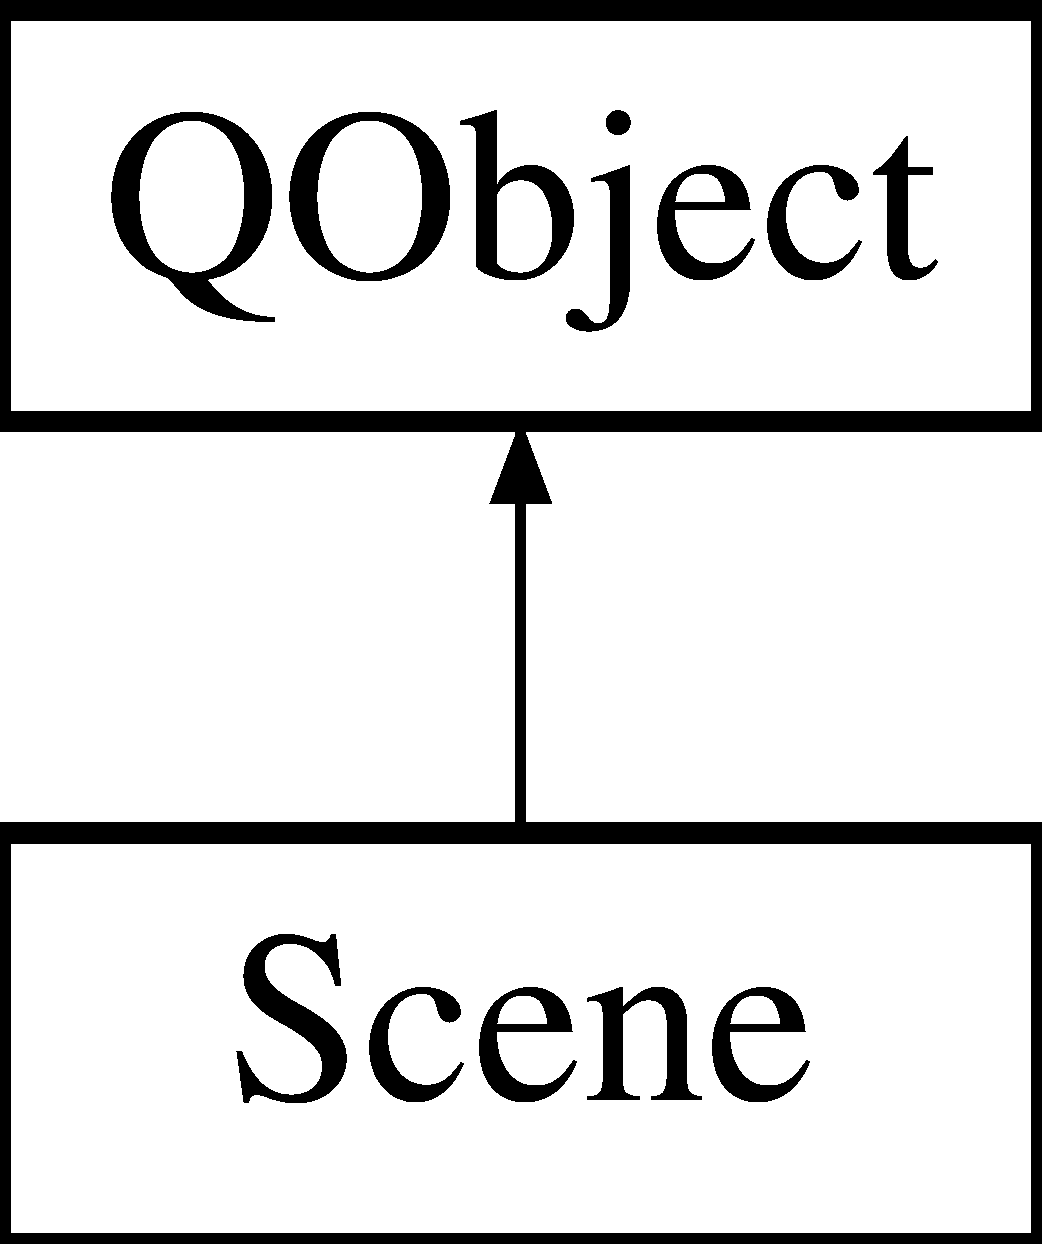
\includegraphics[height=2.000000cm]{class_scene}
\end{center}
\end{figure}
\subsection*{Metody publiczne}
\begin{DoxyCompactItemize}
\item 
\hyperlink{class_scene_aa138923bf1d204f6cadbefbe7398d599}{Scene} (Qt3\+D\+Core\+::\+Q\+Entity $\ast$root\+Entity, \hyperlink{class_main_window}{Main\+Window} \&p\+\_\+main\+Window)
\item 
\hyperlink{class_scene_a3b8cec2e32546713915f8c6303c951f1}{$\sim$\+Scene} ()
\item 
void \hyperlink{class_scene_ae58cf344ad78420d37acde7984c9a4e8}{Set\+Hand\+Transformation} (Q\+Vector$<$ Q\+Vector$<$ float $>$$>$ p\+\_\+\+Finger\+Angles)
\item 
void \hyperlink{class_scene_a4dcd24690f433927c6ca75e9980afd53}{Set\+Hand\+Fingertip\+Values} (Q\+Vector$<$ int $>$ p\+\_\+\+New\+Values)
\end{DoxyCompactItemize}
\subsection*{Atrybuty prywatne}
\begin{DoxyCompactItemize}
\item 
Qt3\+D\+Core\+::\+Q\+Entity $\ast$ \hyperlink{class_scene_a1ef7f61aed73e150dfb7ef7ffc47f7c2}{m\+\_\+root\+Entity}
\item 
\hyperlink{class_hand}{Hand} \hyperlink{class_scene_adf272488e380e731a1c20fa5cd208490}{m\+\_\+\+Hand3\+D\+Model}
\item 
Qt3\+D\+Extras\+::\+Qt3\+D\+Window $\ast$ \hyperlink{class_scene_a3b76fefe111a22aa56f066783fa76bc1}{view}
\item 
Q\+Widget $\ast$ \hyperlink{class_scene_a10832d33619bdb86c51bb75377ea649d}{container}
\item 
Q\+Size \hyperlink{class_scene_a2bb58c1253bd4d64781a2b9e25604060}{screen\+Size}
\item 
Q\+Widget $\ast$ \hyperlink{class_scene_aa6f9d0915a83b6d5e5083c439627ff06}{widget}
\item 
Q\+H\+Box\+Layout $\ast$ \hyperlink{class_scene_a285ea7ad07d9419d79fccbde3a9f8388}{h\+Layout}
\item 
Q\+V\+Box\+Layout $\ast$ \hyperlink{class_scene_adae30f81725ed3f2258bee8fe5e90c5d}{v\+Layout}
\item 
Qt3\+D\+Input\+::\+Q\+Input\+Aspect $\ast$ \hyperlink{class_scene_aa17e5d3b3393d6ea4cbbf7ab981b5b62}{input}
\item 
Qt3\+D\+Render\+::\+Q\+Camera $\ast$ \hyperlink{class_scene_aed08c4ba793fa5d32104d47c9cfd2c5c}{camera\+Entity}
\item 
Qt3\+D\+Extras\+::\+Q\+First\+Person\+Camera\+Controller $\ast$ \hyperlink{class_scene_a55d0f4c21e5ac40b4ad53a67bf851ff7}{cam\+Controller}
\item 
Qt3\+D\+Core\+::\+Q\+Entity $\ast$ \hyperlink{class_scene_a932f32946da0283ac184a28cb13f4427}{light\+Entity}
\item 
Qt3\+D\+Render\+::\+Q\+Point\+Light $\ast$ \hyperlink{class_scene_ac2f294ceccf5b708d6dcdd540e51d787}{light}
\item 
Qt3\+D\+Core\+::\+Q\+Transform $\ast$ \hyperlink{class_scene_a24f2698364e45c011a80c51747a62bae}{light\+Transform}
\item 
Qt3\+D\+Core\+::\+Q\+Entity $\ast$ \hyperlink{class_scene_a9ad241dc981470f63bb5d7a5bd25888e}{light\+Entity2}
\item 
Qt3\+D\+Render\+::\+Q\+Point\+Light $\ast$ \hyperlink{class_scene_a7a9feb72cc710357f6166f5ec45369cd}{light2}
\item 
Qt3\+D\+Core\+::\+Q\+Transform $\ast$ \hyperlink{class_scene_af5b3d0a98c256da599ddd8973016b10b}{light\+Transform2}
\end{DoxyCompactItemize}


\subsection{Opis szczegółowy}
Inicjuje trójwymiatowy model ręki zdefioniowany klasą \hyperlink{class_hand}{Hand}, za pomocą biblioteki Qt3D, a także inicjalizuje widok, widget, rozmiar okna, układ, wejście danych, kontroler perspektywy i oświetlenie 

Definicja w linii 30 pliku scene.\+h.



\subsection{Dokumentacja konstruktora i destruktora}
\mbox{\Hypertarget{class_scene_aa138923bf1d204f6cadbefbe7398d599}\label{class_scene_aa138923bf1d204f6cadbefbe7398d599}} 
\index{Scene@{Scene}!Scene@{Scene}}
\index{Scene@{Scene}!Scene@{Scene}}
\subsubsection{\texorpdfstring{Scene()}{Scene()}}
{\footnotesize\ttfamily Scene\+::\+Scene (\begin{DoxyParamCaption}\item[{Qt3\+D\+Core\+::\+Q\+Entity $\ast$}]{root\+Entity,  }\item[{\hyperlink{class_main_window}{Main\+Window} \&}]{p\+\_\+main\+Window }\end{DoxyParamCaption})\hspace{0.3cm}{\ttfamily [explicit]}}



Definicja w linii 3 pliku scene.\+cpp.

\mbox{\Hypertarget{class_scene_a3b8cec2e32546713915f8c6303c951f1}\label{class_scene_a3b8cec2e32546713915f8c6303c951f1}} 
\index{Scene@{Scene}!````~Scene@{$\sim$\+Scene}}
\index{````~Scene@{$\sim$\+Scene}!Scene@{Scene}}
\subsubsection{\texorpdfstring{$\sim$\+Scene()}{~Scene()}}
{\footnotesize\ttfamily Scene\+::$\sim$\+Scene (\begin{DoxyParamCaption}{ }\end{DoxyParamCaption})}



Definicja w linii 59 pliku scene.\+cpp.



\subsection{Dokumentacja funkcji składowych}
\mbox{\Hypertarget{class_scene_a4dcd24690f433927c6ca75e9980afd53}\label{class_scene_a4dcd24690f433927c6ca75e9980afd53}} 
\index{Scene@{Scene}!Set\+Hand\+Fingertip\+Values@{Set\+Hand\+Fingertip\+Values}}
\index{Set\+Hand\+Fingertip\+Values@{Set\+Hand\+Fingertip\+Values}!Scene@{Scene}}
\subsubsection{\texorpdfstring{Set\+Hand\+Fingertip\+Values()}{SetHandFingertipValues()}}
{\footnotesize\ttfamily void Scene\+::\+Set\+Hand\+Fingertip\+Values (\begin{DoxyParamCaption}\item[{Q\+Vector$<$ int $>$}]{p\+\_\+\+New\+Values }\end{DoxyParamCaption})}



Definicja w linii 69 pliku scene.\+cpp.

\mbox{\Hypertarget{class_scene_ae58cf344ad78420d37acde7984c9a4e8}\label{class_scene_ae58cf344ad78420d37acde7984c9a4e8}} 
\index{Scene@{Scene}!Set\+Hand\+Transformation@{Set\+Hand\+Transformation}}
\index{Set\+Hand\+Transformation@{Set\+Hand\+Transformation}!Scene@{Scene}}
\subsubsection{\texorpdfstring{Set\+Hand\+Transformation()}{SetHandTransformation()}}
{\footnotesize\ttfamily void Scene\+::\+Set\+Hand\+Transformation (\begin{DoxyParamCaption}\item[{Q\+Vector$<$ Q\+Vector$<$ float $>$$>$}]{p\+\_\+\+Finger\+Angles }\end{DoxyParamCaption})}



Definicja w linii 64 pliku scene.\+cpp.



\subsection{Dokumentacja atrybutów składowych}
\mbox{\Hypertarget{class_scene_a55d0f4c21e5ac40b4ad53a67bf851ff7}\label{class_scene_a55d0f4c21e5ac40b4ad53a67bf851ff7}} 
\index{Scene@{Scene}!cam\+Controller@{cam\+Controller}}
\index{cam\+Controller@{cam\+Controller}!Scene@{Scene}}
\subsubsection{\texorpdfstring{cam\+Controller}{camController}}
{\footnotesize\ttfamily Qt3\+D\+Extras\+::\+Q\+First\+Person\+Camera\+Controller$\ast$ Scene\+::cam\+Controller\hspace{0.3cm}{\ttfamily [private]}}



Definicja w linii 45 pliku scene.\+h.

\mbox{\Hypertarget{class_scene_aed08c4ba793fa5d32104d47c9cfd2c5c}\label{class_scene_aed08c4ba793fa5d32104d47c9cfd2c5c}} 
\index{Scene@{Scene}!camera\+Entity@{camera\+Entity}}
\index{camera\+Entity@{camera\+Entity}!Scene@{Scene}}
\subsubsection{\texorpdfstring{camera\+Entity}{cameraEntity}}
{\footnotesize\ttfamily Qt3\+D\+Render\+::\+Q\+Camera$\ast$ Scene\+::camera\+Entity\hspace{0.3cm}{\ttfamily [private]}}



Definicja w linii 44 pliku scene.\+h.

\mbox{\Hypertarget{class_scene_a10832d33619bdb86c51bb75377ea649d}\label{class_scene_a10832d33619bdb86c51bb75377ea649d}} 
\index{Scene@{Scene}!container@{container}}
\index{container@{container}!Scene@{Scene}}
\subsubsection{\texorpdfstring{container}{container}}
{\footnotesize\ttfamily Q\+Widget$\ast$ Scene\+::container\hspace{0.3cm}{\ttfamily [private]}}



Definicja w linii 38 pliku scene.\+h.

\mbox{\Hypertarget{class_scene_a285ea7ad07d9419d79fccbde3a9f8388}\label{class_scene_a285ea7ad07d9419d79fccbde3a9f8388}} 
\index{Scene@{Scene}!h\+Layout@{h\+Layout}}
\index{h\+Layout@{h\+Layout}!Scene@{Scene}}
\subsubsection{\texorpdfstring{h\+Layout}{hLayout}}
{\footnotesize\ttfamily Q\+H\+Box\+Layout$\ast$ Scene\+::h\+Layout\hspace{0.3cm}{\ttfamily [private]}}



Definicja w linii 41 pliku scene.\+h.

\mbox{\Hypertarget{class_scene_aa17e5d3b3393d6ea4cbbf7ab981b5b62}\label{class_scene_aa17e5d3b3393d6ea4cbbf7ab981b5b62}} 
\index{Scene@{Scene}!input@{input}}
\index{input@{input}!Scene@{Scene}}
\subsubsection{\texorpdfstring{input}{input}}
{\footnotesize\ttfamily Qt3\+D\+Input\+::\+Q\+Input\+Aspect$\ast$ Scene\+::input\hspace{0.3cm}{\ttfamily [private]}}



Definicja w linii 43 pliku scene.\+h.

\mbox{\Hypertarget{class_scene_ac2f294ceccf5b708d6dcdd540e51d787}\label{class_scene_ac2f294ceccf5b708d6dcdd540e51d787}} 
\index{Scene@{Scene}!light@{light}}
\index{light@{light}!Scene@{Scene}}
\subsubsection{\texorpdfstring{light}{light}}
{\footnotesize\ttfamily Qt3\+D\+Render\+::\+Q\+Point\+Light$\ast$ Scene\+::light\hspace{0.3cm}{\ttfamily [private]}}



Definicja w linii 47 pliku scene.\+h.

\mbox{\Hypertarget{class_scene_a7a9feb72cc710357f6166f5ec45369cd}\label{class_scene_a7a9feb72cc710357f6166f5ec45369cd}} 
\index{Scene@{Scene}!light2@{light2}}
\index{light2@{light2}!Scene@{Scene}}
\subsubsection{\texorpdfstring{light2}{light2}}
{\footnotesize\ttfamily Qt3\+D\+Render\+::\+Q\+Point\+Light$\ast$ Scene\+::light2\hspace{0.3cm}{\ttfamily [private]}}



Definicja w linii 50 pliku scene.\+h.

\mbox{\Hypertarget{class_scene_a932f32946da0283ac184a28cb13f4427}\label{class_scene_a932f32946da0283ac184a28cb13f4427}} 
\index{Scene@{Scene}!light\+Entity@{light\+Entity}}
\index{light\+Entity@{light\+Entity}!Scene@{Scene}}
\subsubsection{\texorpdfstring{light\+Entity}{lightEntity}}
{\footnotesize\ttfamily Qt3\+D\+Core\+::\+Q\+Entity$\ast$ Scene\+::light\+Entity\hspace{0.3cm}{\ttfamily [private]}}



Definicja w linii 46 pliku scene.\+h.

\mbox{\Hypertarget{class_scene_a9ad241dc981470f63bb5d7a5bd25888e}\label{class_scene_a9ad241dc981470f63bb5d7a5bd25888e}} 
\index{Scene@{Scene}!light\+Entity2@{light\+Entity2}}
\index{light\+Entity2@{light\+Entity2}!Scene@{Scene}}
\subsubsection{\texorpdfstring{light\+Entity2}{lightEntity2}}
{\footnotesize\ttfamily Qt3\+D\+Core\+::\+Q\+Entity$\ast$ Scene\+::light\+Entity2\hspace{0.3cm}{\ttfamily [private]}}



Definicja w linii 49 pliku scene.\+h.

\mbox{\Hypertarget{class_scene_a24f2698364e45c011a80c51747a62bae}\label{class_scene_a24f2698364e45c011a80c51747a62bae}} 
\index{Scene@{Scene}!light\+Transform@{light\+Transform}}
\index{light\+Transform@{light\+Transform}!Scene@{Scene}}
\subsubsection{\texorpdfstring{light\+Transform}{lightTransform}}
{\footnotesize\ttfamily Qt3\+D\+Core\+::\+Q\+Transform$\ast$ Scene\+::light\+Transform\hspace{0.3cm}{\ttfamily [private]}}



Definicja w linii 48 pliku scene.\+h.

\mbox{\Hypertarget{class_scene_af5b3d0a98c256da599ddd8973016b10b}\label{class_scene_af5b3d0a98c256da599ddd8973016b10b}} 
\index{Scene@{Scene}!light\+Transform2@{light\+Transform2}}
\index{light\+Transform2@{light\+Transform2}!Scene@{Scene}}
\subsubsection{\texorpdfstring{light\+Transform2}{lightTransform2}}
{\footnotesize\ttfamily Qt3\+D\+Core\+::\+Q\+Transform$\ast$ Scene\+::light\+Transform2\hspace{0.3cm}{\ttfamily [private]}}



Definicja w linii 51 pliku scene.\+h.

\mbox{\Hypertarget{class_scene_adf272488e380e731a1c20fa5cd208490}\label{class_scene_adf272488e380e731a1c20fa5cd208490}} 
\index{Scene@{Scene}!m\+\_\+\+Hand3\+D\+Model@{m\+\_\+\+Hand3\+D\+Model}}
\index{m\+\_\+\+Hand3\+D\+Model@{m\+\_\+\+Hand3\+D\+Model}!Scene@{Scene}}
\subsubsection{\texorpdfstring{m\+\_\+\+Hand3\+D\+Model}{m\_Hand3DModel}}
{\footnotesize\ttfamily \hyperlink{class_hand}{Hand} Scene\+::m\+\_\+\+Hand3\+D\+Model\hspace{0.3cm}{\ttfamily [private]}}



Definicja w linii 35 pliku scene.\+h.

\mbox{\Hypertarget{class_scene_a1ef7f61aed73e150dfb7ef7ffc47f7c2}\label{class_scene_a1ef7f61aed73e150dfb7ef7ffc47f7c2}} 
\index{Scene@{Scene}!m\+\_\+root\+Entity@{m\+\_\+root\+Entity}}
\index{m\+\_\+root\+Entity@{m\+\_\+root\+Entity}!Scene@{Scene}}
\subsubsection{\texorpdfstring{m\+\_\+root\+Entity}{m\_rootEntity}}
{\footnotesize\ttfamily Qt3\+D\+Core\+::\+Q\+Entity$\ast$ Scene\+::m\+\_\+root\+Entity\hspace{0.3cm}{\ttfamily [private]}}



Definicja w linii 34 pliku scene.\+h.

\mbox{\Hypertarget{class_scene_a2bb58c1253bd4d64781a2b9e25604060}\label{class_scene_a2bb58c1253bd4d64781a2b9e25604060}} 
\index{Scene@{Scene}!screen\+Size@{screen\+Size}}
\index{screen\+Size@{screen\+Size}!Scene@{Scene}}
\subsubsection{\texorpdfstring{screen\+Size}{screenSize}}
{\footnotesize\ttfamily Q\+Size Scene\+::screen\+Size\hspace{0.3cm}{\ttfamily [private]}}



Definicja w linii 39 pliku scene.\+h.

\mbox{\Hypertarget{class_scene_a3b76fefe111a22aa56f066783fa76bc1}\label{class_scene_a3b76fefe111a22aa56f066783fa76bc1}} 
\index{Scene@{Scene}!view@{view}}
\index{view@{view}!Scene@{Scene}}
\subsubsection{\texorpdfstring{view}{view}}
{\footnotesize\ttfamily Qt3\+D\+Extras\+::\+Qt3\+D\+Window$\ast$ Scene\+::view\hspace{0.3cm}{\ttfamily [private]}}



Definicja w linii 37 pliku scene.\+h.

\mbox{\Hypertarget{class_scene_adae30f81725ed3f2258bee8fe5e90c5d}\label{class_scene_adae30f81725ed3f2258bee8fe5e90c5d}} 
\index{Scene@{Scene}!v\+Layout@{v\+Layout}}
\index{v\+Layout@{v\+Layout}!Scene@{Scene}}
\subsubsection{\texorpdfstring{v\+Layout}{vLayout}}
{\footnotesize\ttfamily Q\+V\+Box\+Layout$\ast$ Scene\+::v\+Layout\hspace{0.3cm}{\ttfamily [private]}}



Definicja w linii 42 pliku scene.\+h.

\mbox{\Hypertarget{class_scene_aa6f9d0915a83b6d5e5083c439627ff06}\label{class_scene_aa6f9d0915a83b6d5e5083c439627ff06}} 
\index{Scene@{Scene}!widget@{widget}}
\index{widget@{widget}!Scene@{Scene}}
\subsubsection{\texorpdfstring{widget}{widget}}
{\footnotesize\ttfamily Q\+Widget$\ast$ Scene\+::widget\hspace{0.3cm}{\ttfamily [private]}}



Definicja w linii 40 pliku scene.\+h.



Dokumentacja dla tej klasy została wygenerowana z plików\+:\begin{DoxyCompactItemize}
\item 
\hyperlink{scene_8h}{scene.\+h}\item 
\hyperlink{scene_8cpp}{scene.\+cpp}\end{DoxyCompactItemize}

\chapter{Dokumentacja plików}
\hypertarget{chart_8cpp}{}\section{Dokumentacja pliku chart.\+cpp}
\label{chart_8cpp}\index{chart.\+cpp@{chart.\+cpp}}
{\ttfamily \#include \char`\"{}includes.\+h\char`\"{}}\newline
{\ttfamily \#include \char`\"{}chart.\+h\char`\"{}}\newline
{\ttfamily \#include $<$Qt\+Charts/\+Q\+Abstract\+Axis$>$}\newline
{\ttfamily \#include $<$Qt\+Charts/\+Q\+Spline\+Series$>$}\newline
{\ttfamily \#include $<$Qt\+Charts/\+Q\+Line\+Series$>$}\newline
{\ttfamily \#include $<$Qt\+Charts/\+Q\+Value\+Axis$>$}\newline
{\ttfamily \#include $<$Qt\+Core/\+Q\+Time$>$}\newline
{\ttfamily \#include $<$Qt\+Core/\+Q\+Debug$>$}\newline

\hypertarget{chart_8h}{}\section{Dokumentacja pliku chart.\+h}
\label{chart_8h}\index{chart.\+h@{chart.\+h}}


Definicja klasy \hyperlink{class_chart}{Chart}.  


{\ttfamily \#include $<$Qt\+Charts/\+Q\+Chart$>$}\newline
{\ttfamily \#include $<$Qt\+Charts/\+Q\+Spline\+Series$>$}\newline
{\ttfamily \#include $<$Qt\+Charts/\+Q\+Line\+Series$>$}\newline
{\ttfamily \#include $<$Qt\+Core/\+Q\+Timer$>$}\newline
\subsection*{Komponenty}
\begin{DoxyCompactItemize}
\item 
class \hyperlink{class_chart}{Chart}
\begin{DoxyCompactList}\small\item\em Modeluje pojęcie wykresu dynamicznego. \end{DoxyCompactList}\end{DoxyCompactItemize}


\subsection{Opis szczegółowy}
Plik zawiera definicję klasy \hyperlink{class_chart}{Chart}, która jest klasą pochodną klasy Q\+Object 
\hypertarget{chartwindow_8cpp}{}\section{Dokumentacja pliku chartwindow.\+cpp}
\label{chartwindow_8cpp}\index{chartwindow.\+cpp@{chartwindow.\+cpp}}
{\ttfamily \#include \char`\"{}includes.\+h\char`\"{}}\newline
{\ttfamily \#include \char`\"{}chartwindow.\+h\char`\"{}}\newline
{\ttfamily \#include \char`\"{}ui\+\_\+chartwindow.\+h\char`\"{}}\newline

\hypertarget{chartwindow_8h}{}\section{Dokumentacja pliku chartwindow.\+h}
\label{chartwindow_8h}\index{chartwindow.\+h@{chartwindow.\+h}}


Definicja klasy \hyperlink{classchart_window}{chart\+Window}.  


{\ttfamily \#include $<$Q\+Dialog$>$}\newline
{\ttfamily \#include $<$Qt\+Charts/\+Q\+Chart\+View$>$}\newline
{\ttfamily \#include \char`\"{}input.\+h\char`\"{}}\newline
{\ttfamily \#include \char`\"{}chart.\+h\char`\"{}}\newline
\subsection*{Komponenty}
\begin{DoxyCompactItemize}
\item 
class \hyperlink{classchart_window}{chart\+Window}
\begin{DoxyCompactList}\small\item\em Pośredniczy w wyświetlaniu wykresów dynamicznych. \end{DoxyCompactList}\end{DoxyCompactItemize}
\subsection*{Przestrzenie nazw}
\begin{DoxyCompactItemize}
\item 
 \hyperlink{namespace_ui}{Ui}
\end{DoxyCompactItemize}


\subsection{Opis szczegółowy}
Plik zwiera definicję klasy \hyperlink{classchart_window}{chart\+Window}, która jest klasą pochodną klasy Q\+Main\+Window 
\hypertarget{errorhandler_8cpp}{}\section{Dokumentacja pliku errorhandler.\+cpp}
\label{errorhandler_8cpp}\index{errorhandler.\+cpp@{errorhandler.\+cpp}}
{\ttfamily \#include \char`\"{}includes.\+h\char`\"{}}\newline

\hypertarget{errorhandler_8h}{}\section{Dokumentacja pliku errorhandler.\+h}
\label{errorhandler_8h}\index{errorhandler.\+h@{errorhandler.\+h}}


Definicja klasy \hyperlink{class_error_handler}{Error\+Handler}.  


\subsection*{Komponenty}
\begin{DoxyCompactItemize}
\item 
class \hyperlink{class_error_handler}{Error\+Handler}
\begin{DoxyCompactList}\small\item\em Klasa obsługująca błędy i wyjątki. \end{DoxyCompactList}\end{DoxyCompactItemize}


\subsection{Opis szczegółowy}
Plik zawiera definicję klasy \hyperlink{class_error_handler}{Error\+Handler} 
\hypertarget{finger_8cpp}{}\section{Dokumentacja pliku finger.\+cpp}
\label{finger_8cpp}\index{finger.\+cpp@{finger.\+cpp}}
{\ttfamily \#include \char`\"{}includes.\+h\char`\"{}}\newline

\hypertarget{finger_8h}{}\section{Dokumentacja pliku finger.\+h}
\label{finger_8h}\index{finger.\+h@{finger.\+h}}


Definicja klasy \hyperlink{class_finger}{Finger}.  


{\ttfamily \#include $<$Q\+Object$>$}\newline
{\ttfamily \#include $<$Qt3\+D\+Core/\+Q\+Entity$>$}\newline
{\ttfamily \#include $<$Q\+Matrix4x4$>$}\newline
{\ttfamily \#include $<$Q\+Color$>$}\newline
{\ttfamily \#include \char`\"{}joint.\+h\char`\"{}}\newline
{\ttfamily \#include \char`\"{}manipulatorrotational.\+h\char`\"{}}\newline
{\ttfamily \#include \char`\"{}fingertip.\+h\char`\"{}}\newline
\subsection*{Komponenty}
\begin{DoxyCompactItemize}
\item 
class \hyperlink{class_finger}{Finger}
\begin{DoxyCompactList}\small\item\em Modeluje pojęcie palca w przestrzeni trójwymiarowej. \end{DoxyCompactList}\end{DoxyCompactItemize}
\subsection*{Definicje}
\begin{DoxyCompactItemize}
\item 
\#define \hyperlink{finger_8h_a885bf63c93171052fae8cb96bb3c4d78}{F\+I\+N\+G\+E\+R\+\_\+\+J\+O\+I\+N\+T\+S\+\_\+\+C\+O\+U\+NT}~4
\item 
\#define \hyperlink{finger_8h_a2b2006272771cc32df872c49ba12a43f}{F\+I\+N\+G\+E\+R\+\_\+\+R\+A\+D\+I\+US}~1
\item 
\#define \hyperlink{finger_8h_a9f085e9238de631a39b4b79cf0892bb4}{T\+H\+U\+M\+B\+\_\+\+J\+O\+I\+N\+T\+\_\+\+C\+O\+U\+NT}~2
\item 
\#define \hyperlink{finger_8h_ac940f3dadb20642eeac53feae2ac9830}{T\+H\+U\+M\+B\+\_\+\+J\+O\+I\+N\+T0\+\_\+\+L\+E\+N\+G\+TH}~7.\+0f
\item 
\#define \hyperlink{finger_8h_a10c449518b45d30ce155406d78b83749}{T\+H\+U\+M\+B\+\_\+\+J\+O\+I\+N\+T1\+\_\+\+L\+E\+N\+G\+TH}~3.\+0f
\item 
\#define \hyperlink{finger_8h_abfa4f762bf7dc4fc68bb7dde44287ffe}{T\+H\+U\+M\+B\+\_\+\+J\+O\+I\+N\+T2\+\_\+\+L\+E\+N\+G\+TH}~3.\+0f
\item 
\#define \hyperlink{finger_8h_ad44635d4519f0d322165eaecb3786fe4}{I\+N\+D\+E\+X\+\_\+\+J\+O\+I\+N\+T\+\_\+\+C\+O\+U\+NT}~3
\item 
\#define \hyperlink{finger_8h_a01ea2dfbaeaafda37463b3c0aaf92f35}{I\+N\+D\+E\+X\+\_\+\+F\+I\+N\+G\+E\+R\+\_\+\+J\+O\+I\+N\+T0\+\_\+\+L\+E\+N\+G\+TH}~8.\+5f
\item 
\#define \hyperlink{finger_8h_a2102aab8492130fb106606d00eaab723}{I\+N\+D\+E\+X\+\_\+\+F\+I\+N\+G\+E\+R\+\_\+\+J\+O\+I\+N\+T1\+\_\+\+L\+E\+N\+G\+TH}~5.\+0f
\item 
\#define \hyperlink{finger_8h_a97b53ffbe1104c263ab89133b6732cdf}{I\+N\+D\+E\+X\+\_\+\+F\+I\+N\+G\+E\+R\+\_\+\+J\+O\+I\+N\+T2\+\_\+\+L\+E\+N\+G\+TH}~2.\+5f
\item 
\#define \hyperlink{finger_8h_acdaafe23520fd16a305355215bed3749}{I\+N\+D\+E\+X\+\_\+\+F\+I\+N\+G\+E\+R\+\_\+\+J\+O\+I\+N\+T3\+\_\+\+L\+E\+N\+G\+TH}~2.\+0f
\item 
\#define \hyperlink{finger_8h_a06307b66501338bd67a38aef261dfcd9}{M\+I\+D\+D\+L\+E\+\_\+\+J\+O\+I\+N\+T\+\_\+\+C\+O\+U\+NT}~3
\item 
\#define \hyperlink{finger_8h_ab6e8df5ebfd06d0d229bf14a9823d2c1}{M\+I\+D\+D\+L\+E\+\_\+\+F\+I\+N\+G\+E\+R\+\_\+\+J\+O\+I\+N\+T0\+\_\+\+L\+E\+N\+G\+TH}~8.\+0f
\item 
\#define \hyperlink{finger_8h_a26b41c3705e53f7fbe8dea13c0af1147}{M\+I\+D\+D\+L\+E\+\_\+\+F\+I\+N\+G\+E\+R\+\_\+\+J\+O\+I\+N\+T1\+\_\+\+L\+E\+N\+G\+TH}~5.\+3f
\item 
\#define \hyperlink{finger_8h_a8db82d8dc98e7d04e28964c08c0d434b}{M\+I\+D\+D\+L\+E\+\_\+\+F\+I\+N\+G\+E\+R\+\_\+\+J\+O\+I\+N\+T2\+\_\+\+L\+E\+N\+G\+TH}~2.\+8f
\item 
\#define \hyperlink{finger_8h_a0fce84d70985373ac978ebf601e39e49}{M\+I\+D\+D\+L\+E\+\_\+\+F\+I\+N\+G\+E\+R\+\_\+\+J\+O\+I\+N\+T3\+\_\+\+L\+E\+N\+G\+TH}~2.\+3f
\item 
\#define \hyperlink{finger_8h_ac41bcba256383547e600eb73d983a853}{R\+I\+N\+G\+\_\+\+J\+O\+I\+N\+T\+\_\+\+C\+O\+U\+NT}~3
\item 
\#define \hyperlink{finger_8h_ad3103c1b2dc6dfa368a7e30871db3052}{R\+I\+N\+G\+\_\+\+F\+I\+N\+G\+E\+R\+\_\+\+J\+O\+I\+N\+T0\+\_\+\+L\+E\+N\+G\+TH}~7.\+5f
\item 
\#define \hyperlink{finger_8h_a31f1e18033c92678ccd6efbe6e638b12}{R\+I\+N\+G\+\_\+\+F\+I\+N\+G\+E\+R\+\_\+\+J\+O\+I\+N\+T1\+\_\+\+L\+E\+N\+G\+TH}~4.\+5f
\item 
\#define \hyperlink{finger_8h_af17312bf7e290e1a4d0debf530c63453}{R\+I\+N\+G\+\_\+\+F\+I\+N\+G\+E\+R\+\_\+\+J\+O\+I\+N\+T2\+\_\+\+L\+E\+N\+G\+TH}~2.\+8f
\item 
\#define \hyperlink{finger_8h_ae0b222cd8298fcfb0cf06b50313e6db8}{R\+I\+N\+G\+\_\+\+F\+I\+N\+G\+E\+R\+\_\+\+J\+O\+I\+N\+T3\+\_\+\+L\+E\+N\+G\+TH}~2.\+4f
\item 
\#define \hyperlink{finger_8h_aa552bc1ad566696421ddf748dd65c2ce}{P\+I\+N\+K\+Y\+\_\+\+J\+O\+I\+N\+T\+\_\+\+C\+O\+U\+NT}~3
\item 
\#define \hyperlink{finger_8h_af6a038b34388ad3a97e7ed26e2729c06}{P\+I\+N\+K\+Y\+\_\+\+J\+O\+I\+N\+T0\+\_\+\+L\+E\+N\+G\+TH}~6.\+3f
\item 
\#define \hyperlink{finger_8h_a5c52f20a1e362e43f5277c05204b04e7}{P\+I\+N\+K\+Y\+\_\+\+J\+O\+I\+N\+T1\+\_\+\+L\+E\+N\+G\+TH}~3.\+3f
\item 
\#define \hyperlink{finger_8h_a4a82cdb558799dbc92cfb55a97b2cda5}{P\+I\+N\+K\+Y\+\_\+\+J\+O\+I\+N\+T2\+\_\+\+L\+E\+N\+G\+TH}~2.\+0f
\item 
\#define \hyperlink{finger_8h_a58094f7e0358c5ab3ffacfd21a71955a}{P\+I\+N\+K\+Y\+\_\+\+J\+O\+I\+N\+T3\+\_\+\+L\+E\+N\+G\+TH}~2.\+3f
\end{DoxyCompactItemize}


\subsection{Opis szczegółowy}
Plik zawiera definicję klasy finger, która jest klasą pochodną klasy Q\+Object 

\subsection{Dokumentacja definicji}
\mbox{\Hypertarget{finger_8h_a885bf63c93171052fae8cb96bb3c4d78}\label{finger_8h_a885bf63c93171052fae8cb96bb3c4d78}} 
\index{finger.\+h@{finger.\+h}!F\+I\+N\+G\+E\+R\+\_\+\+J\+O\+I\+N\+T\+S\+\_\+\+C\+O\+U\+NT@{F\+I\+N\+G\+E\+R\+\_\+\+J\+O\+I\+N\+T\+S\+\_\+\+C\+O\+U\+NT}}
\index{F\+I\+N\+G\+E\+R\+\_\+\+J\+O\+I\+N\+T\+S\+\_\+\+C\+O\+U\+NT@{F\+I\+N\+G\+E\+R\+\_\+\+J\+O\+I\+N\+T\+S\+\_\+\+C\+O\+U\+NT}!finger.\+h@{finger.\+h}}
\subsubsection{\texorpdfstring{F\+I\+N\+G\+E\+R\+\_\+\+J\+O\+I\+N\+T\+S\+\_\+\+C\+O\+U\+NT}{FINGER\_JOINTS\_COUNT}}
{\footnotesize\ttfamily \#define F\+I\+N\+G\+E\+R\+\_\+\+J\+O\+I\+N\+T\+S\+\_\+\+C\+O\+U\+NT~4}



Definicja w linii 12 pliku finger.\+h.

\mbox{\Hypertarget{finger_8h_a2b2006272771cc32df872c49ba12a43f}\label{finger_8h_a2b2006272771cc32df872c49ba12a43f}} 
\index{finger.\+h@{finger.\+h}!F\+I\+N\+G\+E\+R\+\_\+\+R\+A\+D\+I\+US@{F\+I\+N\+G\+E\+R\+\_\+\+R\+A\+D\+I\+US}}
\index{F\+I\+N\+G\+E\+R\+\_\+\+R\+A\+D\+I\+US@{F\+I\+N\+G\+E\+R\+\_\+\+R\+A\+D\+I\+US}!finger.\+h@{finger.\+h}}
\subsubsection{\texorpdfstring{F\+I\+N\+G\+E\+R\+\_\+\+R\+A\+D\+I\+US}{FINGER\_RADIUS}}
{\footnotesize\ttfamily \#define F\+I\+N\+G\+E\+R\+\_\+\+R\+A\+D\+I\+US~1}



Definicja w linii 13 pliku finger.\+h.

\mbox{\Hypertarget{finger_8h_a01ea2dfbaeaafda37463b3c0aaf92f35}\label{finger_8h_a01ea2dfbaeaafda37463b3c0aaf92f35}} 
\index{finger.\+h@{finger.\+h}!I\+N\+D\+E\+X\+\_\+\+F\+I\+N\+G\+E\+R\+\_\+\+J\+O\+I\+N\+T0\+\_\+\+L\+E\+N\+G\+TH@{I\+N\+D\+E\+X\+\_\+\+F\+I\+N\+G\+E\+R\+\_\+\+J\+O\+I\+N\+T0\+\_\+\+L\+E\+N\+G\+TH}}
\index{I\+N\+D\+E\+X\+\_\+\+F\+I\+N\+G\+E\+R\+\_\+\+J\+O\+I\+N\+T0\+\_\+\+L\+E\+N\+G\+TH@{I\+N\+D\+E\+X\+\_\+\+F\+I\+N\+G\+E\+R\+\_\+\+J\+O\+I\+N\+T0\+\_\+\+L\+E\+N\+G\+TH}!finger.\+h@{finger.\+h}}
\subsubsection{\texorpdfstring{I\+N\+D\+E\+X\+\_\+\+F\+I\+N\+G\+E\+R\+\_\+\+J\+O\+I\+N\+T0\+\_\+\+L\+E\+N\+G\+TH}{INDEX\_FINGER\_JOINT0\_LENGTH}}
{\footnotesize\ttfamily \#define I\+N\+D\+E\+X\+\_\+\+F\+I\+N\+G\+E\+R\+\_\+\+J\+O\+I\+N\+T0\+\_\+\+L\+E\+N\+G\+TH~8.\+5f}



Definicja w linii 21 pliku finger.\+h.

\mbox{\Hypertarget{finger_8h_a2102aab8492130fb106606d00eaab723}\label{finger_8h_a2102aab8492130fb106606d00eaab723}} 
\index{finger.\+h@{finger.\+h}!I\+N\+D\+E\+X\+\_\+\+F\+I\+N\+G\+E\+R\+\_\+\+J\+O\+I\+N\+T1\+\_\+\+L\+E\+N\+G\+TH@{I\+N\+D\+E\+X\+\_\+\+F\+I\+N\+G\+E\+R\+\_\+\+J\+O\+I\+N\+T1\+\_\+\+L\+E\+N\+G\+TH}}
\index{I\+N\+D\+E\+X\+\_\+\+F\+I\+N\+G\+E\+R\+\_\+\+J\+O\+I\+N\+T1\+\_\+\+L\+E\+N\+G\+TH@{I\+N\+D\+E\+X\+\_\+\+F\+I\+N\+G\+E\+R\+\_\+\+J\+O\+I\+N\+T1\+\_\+\+L\+E\+N\+G\+TH}!finger.\+h@{finger.\+h}}
\subsubsection{\texorpdfstring{I\+N\+D\+E\+X\+\_\+\+F\+I\+N\+G\+E\+R\+\_\+\+J\+O\+I\+N\+T1\+\_\+\+L\+E\+N\+G\+TH}{INDEX\_FINGER\_JOINT1\_LENGTH}}
{\footnotesize\ttfamily \#define I\+N\+D\+E\+X\+\_\+\+F\+I\+N\+G\+E\+R\+\_\+\+J\+O\+I\+N\+T1\+\_\+\+L\+E\+N\+G\+TH~5.\+0f}



Definicja w linii 22 pliku finger.\+h.

\mbox{\Hypertarget{finger_8h_a97b53ffbe1104c263ab89133b6732cdf}\label{finger_8h_a97b53ffbe1104c263ab89133b6732cdf}} 
\index{finger.\+h@{finger.\+h}!I\+N\+D\+E\+X\+\_\+\+F\+I\+N\+G\+E\+R\+\_\+\+J\+O\+I\+N\+T2\+\_\+\+L\+E\+N\+G\+TH@{I\+N\+D\+E\+X\+\_\+\+F\+I\+N\+G\+E\+R\+\_\+\+J\+O\+I\+N\+T2\+\_\+\+L\+E\+N\+G\+TH}}
\index{I\+N\+D\+E\+X\+\_\+\+F\+I\+N\+G\+E\+R\+\_\+\+J\+O\+I\+N\+T2\+\_\+\+L\+E\+N\+G\+TH@{I\+N\+D\+E\+X\+\_\+\+F\+I\+N\+G\+E\+R\+\_\+\+J\+O\+I\+N\+T2\+\_\+\+L\+E\+N\+G\+TH}!finger.\+h@{finger.\+h}}
\subsubsection{\texorpdfstring{I\+N\+D\+E\+X\+\_\+\+F\+I\+N\+G\+E\+R\+\_\+\+J\+O\+I\+N\+T2\+\_\+\+L\+E\+N\+G\+TH}{INDEX\_FINGER\_JOINT2\_LENGTH}}
{\footnotesize\ttfamily \#define I\+N\+D\+E\+X\+\_\+\+F\+I\+N\+G\+E\+R\+\_\+\+J\+O\+I\+N\+T2\+\_\+\+L\+E\+N\+G\+TH~2.\+5f}



Definicja w linii 23 pliku finger.\+h.

\mbox{\Hypertarget{finger_8h_acdaafe23520fd16a305355215bed3749}\label{finger_8h_acdaafe23520fd16a305355215bed3749}} 
\index{finger.\+h@{finger.\+h}!I\+N\+D\+E\+X\+\_\+\+F\+I\+N\+G\+E\+R\+\_\+\+J\+O\+I\+N\+T3\+\_\+\+L\+E\+N\+G\+TH@{I\+N\+D\+E\+X\+\_\+\+F\+I\+N\+G\+E\+R\+\_\+\+J\+O\+I\+N\+T3\+\_\+\+L\+E\+N\+G\+TH}}
\index{I\+N\+D\+E\+X\+\_\+\+F\+I\+N\+G\+E\+R\+\_\+\+J\+O\+I\+N\+T3\+\_\+\+L\+E\+N\+G\+TH@{I\+N\+D\+E\+X\+\_\+\+F\+I\+N\+G\+E\+R\+\_\+\+J\+O\+I\+N\+T3\+\_\+\+L\+E\+N\+G\+TH}!finger.\+h@{finger.\+h}}
\subsubsection{\texorpdfstring{I\+N\+D\+E\+X\+\_\+\+F\+I\+N\+G\+E\+R\+\_\+\+J\+O\+I\+N\+T3\+\_\+\+L\+E\+N\+G\+TH}{INDEX\_FINGER\_JOINT3\_LENGTH}}
{\footnotesize\ttfamily \#define I\+N\+D\+E\+X\+\_\+\+F\+I\+N\+G\+E\+R\+\_\+\+J\+O\+I\+N\+T3\+\_\+\+L\+E\+N\+G\+TH~2.\+0f}



Definicja w linii 24 pliku finger.\+h.

\mbox{\Hypertarget{finger_8h_ad44635d4519f0d322165eaecb3786fe4}\label{finger_8h_ad44635d4519f0d322165eaecb3786fe4}} 
\index{finger.\+h@{finger.\+h}!I\+N\+D\+E\+X\+\_\+\+J\+O\+I\+N\+T\+\_\+\+C\+O\+U\+NT@{I\+N\+D\+E\+X\+\_\+\+J\+O\+I\+N\+T\+\_\+\+C\+O\+U\+NT}}
\index{I\+N\+D\+E\+X\+\_\+\+J\+O\+I\+N\+T\+\_\+\+C\+O\+U\+NT@{I\+N\+D\+E\+X\+\_\+\+J\+O\+I\+N\+T\+\_\+\+C\+O\+U\+NT}!finger.\+h@{finger.\+h}}
\subsubsection{\texorpdfstring{I\+N\+D\+E\+X\+\_\+\+J\+O\+I\+N\+T\+\_\+\+C\+O\+U\+NT}{INDEX\_JOINT\_COUNT}}
{\footnotesize\ttfamily \#define I\+N\+D\+E\+X\+\_\+\+J\+O\+I\+N\+T\+\_\+\+C\+O\+U\+NT~3}



Definicja w linii 20 pliku finger.\+h.

\mbox{\Hypertarget{finger_8h_ab6e8df5ebfd06d0d229bf14a9823d2c1}\label{finger_8h_ab6e8df5ebfd06d0d229bf14a9823d2c1}} 
\index{finger.\+h@{finger.\+h}!M\+I\+D\+D\+L\+E\+\_\+\+F\+I\+N\+G\+E\+R\+\_\+\+J\+O\+I\+N\+T0\+\_\+\+L\+E\+N\+G\+TH@{M\+I\+D\+D\+L\+E\+\_\+\+F\+I\+N\+G\+E\+R\+\_\+\+J\+O\+I\+N\+T0\+\_\+\+L\+E\+N\+G\+TH}}
\index{M\+I\+D\+D\+L\+E\+\_\+\+F\+I\+N\+G\+E\+R\+\_\+\+J\+O\+I\+N\+T0\+\_\+\+L\+E\+N\+G\+TH@{M\+I\+D\+D\+L\+E\+\_\+\+F\+I\+N\+G\+E\+R\+\_\+\+J\+O\+I\+N\+T0\+\_\+\+L\+E\+N\+G\+TH}!finger.\+h@{finger.\+h}}
\subsubsection{\texorpdfstring{M\+I\+D\+D\+L\+E\+\_\+\+F\+I\+N\+G\+E\+R\+\_\+\+J\+O\+I\+N\+T0\+\_\+\+L\+E\+N\+G\+TH}{MIDDLE\_FINGER\_JOINT0\_LENGTH}}
{\footnotesize\ttfamily \#define M\+I\+D\+D\+L\+E\+\_\+\+F\+I\+N\+G\+E\+R\+\_\+\+J\+O\+I\+N\+T0\+\_\+\+L\+E\+N\+G\+TH~8.\+0f}



Definicja w linii 27 pliku finger.\+h.

\mbox{\Hypertarget{finger_8h_a26b41c3705e53f7fbe8dea13c0af1147}\label{finger_8h_a26b41c3705e53f7fbe8dea13c0af1147}} 
\index{finger.\+h@{finger.\+h}!M\+I\+D\+D\+L\+E\+\_\+\+F\+I\+N\+G\+E\+R\+\_\+\+J\+O\+I\+N\+T1\+\_\+\+L\+E\+N\+G\+TH@{M\+I\+D\+D\+L\+E\+\_\+\+F\+I\+N\+G\+E\+R\+\_\+\+J\+O\+I\+N\+T1\+\_\+\+L\+E\+N\+G\+TH}}
\index{M\+I\+D\+D\+L\+E\+\_\+\+F\+I\+N\+G\+E\+R\+\_\+\+J\+O\+I\+N\+T1\+\_\+\+L\+E\+N\+G\+TH@{M\+I\+D\+D\+L\+E\+\_\+\+F\+I\+N\+G\+E\+R\+\_\+\+J\+O\+I\+N\+T1\+\_\+\+L\+E\+N\+G\+TH}!finger.\+h@{finger.\+h}}
\subsubsection{\texorpdfstring{M\+I\+D\+D\+L\+E\+\_\+\+F\+I\+N\+G\+E\+R\+\_\+\+J\+O\+I\+N\+T1\+\_\+\+L\+E\+N\+G\+TH}{MIDDLE\_FINGER\_JOINT1\_LENGTH}}
{\footnotesize\ttfamily \#define M\+I\+D\+D\+L\+E\+\_\+\+F\+I\+N\+G\+E\+R\+\_\+\+J\+O\+I\+N\+T1\+\_\+\+L\+E\+N\+G\+TH~5.\+3f}



Definicja w linii 28 pliku finger.\+h.

\mbox{\Hypertarget{finger_8h_a8db82d8dc98e7d04e28964c08c0d434b}\label{finger_8h_a8db82d8dc98e7d04e28964c08c0d434b}} 
\index{finger.\+h@{finger.\+h}!M\+I\+D\+D\+L\+E\+\_\+\+F\+I\+N\+G\+E\+R\+\_\+\+J\+O\+I\+N\+T2\+\_\+\+L\+E\+N\+G\+TH@{M\+I\+D\+D\+L\+E\+\_\+\+F\+I\+N\+G\+E\+R\+\_\+\+J\+O\+I\+N\+T2\+\_\+\+L\+E\+N\+G\+TH}}
\index{M\+I\+D\+D\+L\+E\+\_\+\+F\+I\+N\+G\+E\+R\+\_\+\+J\+O\+I\+N\+T2\+\_\+\+L\+E\+N\+G\+TH@{M\+I\+D\+D\+L\+E\+\_\+\+F\+I\+N\+G\+E\+R\+\_\+\+J\+O\+I\+N\+T2\+\_\+\+L\+E\+N\+G\+TH}!finger.\+h@{finger.\+h}}
\subsubsection{\texorpdfstring{M\+I\+D\+D\+L\+E\+\_\+\+F\+I\+N\+G\+E\+R\+\_\+\+J\+O\+I\+N\+T2\+\_\+\+L\+E\+N\+G\+TH}{MIDDLE\_FINGER\_JOINT2\_LENGTH}}
{\footnotesize\ttfamily \#define M\+I\+D\+D\+L\+E\+\_\+\+F\+I\+N\+G\+E\+R\+\_\+\+J\+O\+I\+N\+T2\+\_\+\+L\+E\+N\+G\+TH~2.\+8f}



Definicja w linii 29 pliku finger.\+h.

\mbox{\Hypertarget{finger_8h_a0fce84d70985373ac978ebf601e39e49}\label{finger_8h_a0fce84d70985373ac978ebf601e39e49}} 
\index{finger.\+h@{finger.\+h}!M\+I\+D\+D\+L\+E\+\_\+\+F\+I\+N\+G\+E\+R\+\_\+\+J\+O\+I\+N\+T3\+\_\+\+L\+E\+N\+G\+TH@{M\+I\+D\+D\+L\+E\+\_\+\+F\+I\+N\+G\+E\+R\+\_\+\+J\+O\+I\+N\+T3\+\_\+\+L\+E\+N\+G\+TH}}
\index{M\+I\+D\+D\+L\+E\+\_\+\+F\+I\+N\+G\+E\+R\+\_\+\+J\+O\+I\+N\+T3\+\_\+\+L\+E\+N\+G\+TH@{M\+I\+D\+D\+L\+E\+\_\+\+F\+I\+N\+G\+E\+R\+\_\+\+J\+O\+I\+N\+T3\+\_\+\+L\+E\+N\+G\+TH}!finger.\+h@{finger.\+h}}
\subsubsection{\texorpdfstring{M\+I\+D\+D\+L\+E\+\_\+\+F\+I\+N\+G\+E\+R\+\_\+\+J\+O\+I\+N\+T3\+\_\+\+L\+E\+N\+G\+TH}{MIDDLE\_FINGER\_JOINT3\_LENGTH}}
{\footnotesize\ttfamily \#define M\+I\+D\+D\+L\+E\+\_\+\+F\+I\+N\+G\+E\+R\+\_\+\+J\+O\+I\+N\+T3\+\_\+\+L\+E\+N\+G\+TH~2.\+3f}



Definicja w linii 30 pliku finger.\+h.

\mbox{\Hypertarget{finger_8h_a06307b66501338bd67a38aef261dfcd9}\label{finger_8h_a06307b66501338bd67a38aef261dfcd9}} 
\index{finger.\+h@{finger.\+h}!M\+I\+D\+D\+L\+E\+\_\+\+J\+O\+I\+N\+T\+\_\+\+C\+O\+U\+NT@{M\+I\+D\+D\+L\+E\+\_\+\+J\+O\+I\+N\+T\+\_\+\+C\+O\+U\+NT}}
\index{M\+I\+D\+D\+L\+E\+\_\+\+J\+O\+I\+N\+T\+\_\+\+C\+O\+U\+NT@{M\+I\+D\+D\+L\+E\+\_\+\+J\+O\+I\+N\+T\+\_\+\+C\+O\+U\+NT}!finger.\+h@{finger.\+h}}
\subsubsection{\texorpdfstring{M\+I\+D\+D\+L\+E\+\_\+\+J\+O\+I\+N\+T\+\_\+\+C\+O\+U\+NT}{MIDDLE\_JOINT\_COUNT}}
{\footnotesize\ttfamily \#define M\+I\+D\+D\+L\+E\+\_\+\+J\+O\+I\+N\+T\+\_\+\+C\+O\+U\+NT~3}



Definicja w linii 26 pliku finger.\+h.

\mbox{\Hypertarget{finger_8h_af6a038b34388ad3a97e7ed26e2729c06}\label{finger_8h_af6a038b34388ad3a97e7ed26e2729c06}} 
\index{finger.\+h@{finger.\+h}!P\+I\+N\+K\+Y\+\_\+\+J\+O\+I\+N\+T0\+\_\+\+L\+E\+N\+G\+TH@{P\+I\+N\+K\+Y\+\_\+\+J\+O\+I\+N\+T0\+\_\+\+L\+E\+N\+G\+TH}}
\index{P\+I\+N\+K\+Y\+\_\+\+J\+O\+I\+N\+T0\+\_\+\+L\+E\+N\+G\+TH@{P\+I\+N\+K\+Y\+\_\+\+J\+O\+I\+N\+T0\+\_\+\+L\+E\+N\+G\+TH}!finger.\+h@{finger.\+h}}
\subsubsection{\texorpdfstring{P\+I\+N\+K\+Y\+\_\+\+J\+O\+I\+N\+T0\+\_\+\+L\+E\+N\+G\+TH}{PINKY\_JOINT0\_LENGTH}}
{\footnotesize\ttfamily \#define P\+I\+N\+K\+Y\+\_\+\+J\+O\+I\+N\+T0\+\_\+\+L\+E\+N\+G\+TH~6.\+3f}



Definicja w linii 39 pliku finger.\+h.

\mbox{\Hypertarget{finger_8h_a5c52f20a1e362e43f5277c05204b04e7}\label{finger_8h_a5c52f20a1e362e43f5277c05204b04e7}} 
\index{finger.\+h@{finger.\+h}!P\+I\+N\+K\+Y\+\_\+\+J\+O\+I\+N\+T1\+\_\+\+L\+E\+N\+G\+TH@{P\+I\+N\+K\+Y\+\_\+\+J\+O\+I\+N\+T1\+\_\+\+L\+E\+N\+G\+TH}}
\index{P\+I\+N\+K\+Y\+\_\+\+J\+O\+I\+N\+T1\+\_\+\+L\+E\+N\+G\+TH@{P\+I\+N\+K\+Y\+\_\+\+J\+O\+I\+N\+T1\+\_\+\+L\+E\+N\+G\+TH}!finger.\+h@{finger.\+h}}
\subsubsection{\texorpdfstring{P\+I\+N\+K\+Y\+\_\+\+J\+O\+I\+N\+T1\+\_\+\+L\+E\+N\+G\+TH}{PINKY\_JOINT1\_LENGTH}}
{\footnotesize\ttfamily \#define P\+I\+N\+K\+Y\+\_\+\+J\+O\+I\+N\+T1\+\_\+\+L\+E\+N\+G\+TH~3.\+3f}



Definicja w linii 40 pliku finger.\+h.

\mbox{\Hypertarget{finger_8h_a4a82cdb558799dbc92cfb55a97b2cda5}\label{finger_8h_a4a82cdb558799dbc92cfb55a97b2cda5}} 
\index{finger.\+h@{finger.\+h}!P\+I\+N\+K\+Y\+\_\+\+J\+O\+I\+N\+T2\+\_\+\+L\+E\+N\+G\+TH@{P\+I\+N\+K\+Y\+\_\+\+J\+O\+I\+N\+T2\+\_\+\+L\+E\+N\+G\+TH}}
\index{P\+I\+N\+K\+Y\+\_\+\+J\+O\+I\+N\+T2\+\_\+\+L\+E\+N\+G\+TH@{P\+I\+N\+K\+Y\+\_\+\+J\+O\+I\+N\+T2\+\_\+\+L\+E\+N\+G\+TH}!finger.\+h@{finger.\+h}}
\subsubsection{\texorpdfstring{P\+I\+N\+K\+Y\+\_\+\+J\+O\+I\+N\+T2\+\_\+\+L\+E\+N\+G\+TH}{PINKY\_JOINT2\_LENGTH}}
{\footnotesize\ttfamily \#define P\+I\+N\+K\+Y\+\_\+\+J\+O\+I\+N\+T2\+\_\+\+L\+E\+N\+G\+TH~2.\+0f}



Definicja w linii 41 pliku finger.\+h.

\mbox{\Hypertarget{finger_8h_a58094f7e0358c5ab3ffacfd21a71955a}\label{finger_8h_a58094f7e0358c5ab3ffacfd21a71955a}} 
\index{finger.\+h@{finger.\+h}!P\+I\+N\+K\+Y\+\_\+\+J\+O\+I\+N\+T3\+\_\+\+L\+E\+N\+G\+TH@{P\+I\+N\+K\+Y\+\_\+\+J\+O\+I\+N\+T3\+\_\+\+L\+E\+N\+G\+TH}}
\index{P\+I\+N\+K\+Y\+\_\+\+J\+O\+I\+N\+T3\+\_\+\+L\+E\+N\+G\+TH@{P\+I\+N\+K\+Y\+\_\+\+J\+O\+I\+N\+T3\+\_\+\+L\+E\+N\+G\+TH}!finger.\+h@{finger.\+h}}
\subsubsection{\texorpdfstring{P\+I\+N\+K\+Y\+\_\+\+J\+O\+I\+N\+T3\+\_\+\+L\+E\+N\+G\+TH}{PINKY\_JOINT3\_LENGTH}}
{\footnotesize\ttfamily \#define P\+I\+N\+K\+Y\+\_\+\+J\+O\+I\+N\+T3\+\_\+\+L\+E\+N\+G\+TH~2.\+3f}



Definicja w linii 42 pliku finger.\+h.

\mbox{\Hypertarget{finger_8h_aa552bc1ad566696421ddf748dd65c2ce}\label{finger_8h_aa552bc1ad566696421ddf748dd65c2ce}} 
\index{finger.\+h@{finger.\+h}!P\+I\+N\+K\+Y\+\_\+\+J\+O\+I\+N\+T\+\_\+\+C\+O\+U\+NT@{P\+I\+N\+K\+Y\+\_\+\+J\+O\+I\+N\+T\+\_\+\+C\+O\+U\+NT}}
\index{P\+I\+N\+K\+Y\+\_\+\+J\+O\+I\+N\+T\+\_\+\+C\+O\+U\+NT@{P\+I\+N\+K\+Y\+\_\+\+J\+O\+I\+N\+T\+\_\+\+C\+O\+U\+NT}!finger.\+h@{finger.\+h}}
\subsubsection{\texorpdfstring{P\+I\+N\+K\+Y\+\_\+\+J\+O\+I\+N\+T\+\_\+\+C\+O\+U\+NT}{PINKY\_JOINT\_COUNT}}
{\footnotesize\ttfamily \#define P\+I\+N\+K\+Y\+\_\+\+J\+O\+I\+N\+T\+\_\+\+C\+O\+U\+NT~3}



Definicja w linii 38 pliku finger.\+h.

\mbox{\Hypertarget{finger_8h_ad3103c1b2dc6dfa368a7e30871db3052}\label{finger_8h_ad3103c1b2dc6dfa368a7e30871db3052}} 
\index{finger.\+h@{finger.\+h}!R\+I\+N\+G\+\_\+\+F\+I\+N\+G\+E\+R\+\_\+\+J\+O\+I\+N\+T0\+\_\+\+L\+E\+N\+G\+TH@{R\+I\+N\+G\+\_\+\+F\+I\+N\+G\+E\+R\+\_\+\+J\+O\+I\+N\+T0\+\_\+\+L\+E\+N\+G\+TH}}
\index{R\+I\+N\+G\+\_\+\+F\+I\+N\+G\+E\+R\+\_\+\+J\+O\+I\+N\+T0\+\_\+\+L\+E\+N\+G\+TH@{R\+I\+N\+G\+\_\+\+F\+I\+N\+G\+E\+R\+\_\+\+J\+O\+I\+N\+T0\+\_\+\+L\+E\+N\+G\+TH}!finger.\+h@{finger.\+h}}
\subsubsection{\texorpdfstring{R\+I\+N\+G\+\_\+\+F\+I\+N\+G\+E\+R\+\_\+\+J\+O\+I\+N\+T0\+\_\+\+L\+E\+N\+G\+TH}{RING\_FINGER\_JOINT0\_LENGTH}}
{\footnotesize\ttfamily \#define R\+I\+N\+G\+\_\+\+F\+I\+N\+G\+E\+R\+\_\+\+J\+O\+I\+N\+T0\+\_\+\+L\+E\+N\+G\+TH~7.\+5f}



Definicja w linii 33 pliku finger.\+h.

\mbox{\Hypertarget{finger_8h_a31f1e18033c92678ccd6efbe6e638b12}\label{finger_8h_a31f1e18033c92678ccd6efbe6e638b12}} 
\index{finger.\+h@{finger.\+h}!R\+I\+N\+G\+\_\+\+F\+I\+N\+G\+E\+R\+\_\+\+J\+O\+I\+N\+T1\+\_\+\+L\+E\+N\+G\+TH@{R\+I\+N\+G\+\_\+\+F\+I\+N\+G\+E\+R\+\_\+\+J\+O\+I\+N\+T1\+\_\+\+L\+E\+N\+G\+TH}}
\index{R\+I\+N\+G\+\_\+\+F\+I\+N\+G\+E\+R\+\_\+\+J\+O\+I\+N\+T1\+\_\+\+L\+E\+N\+G\+TH@{R\+I\+N\+G\+\_\+\+F\+I\+N\+G\+E\+R\+\_\+\+J\+O\+I\+N\+T1\+\_\+\+L\+E\+N\+G\+TH}!finger.\+h@{finger.\+h}}
\subsubsection{\texorpdfstring{R\+I\+N\+G\+\_\+\+F\+I\+N\+G\+E\+R\+\_\+\+J\+O\+I\+N\+T1\+\_\+\+L\+E\+N\+G\+TH}{RING\_FINGER\_JOINT1\_LENGTH}}
{\footnotesize\ttfamily \#define R\+I\+N\+G\+\_\+\+F\+I\+N\+G\+E\+R\+\_\+\+J\+O\+I\+N\+T1\+\_\+\+L\+E\+N\+G\+TH~4.\+5f}



Definicja w linii 34 pliku finger.\+h.

\mbox{\Hypertarget{finger_8h_af17312bf7e290e1a4d0debf530c63453}\label{finger_8h_af17312bf7e290e1a4d0debf530c63453}} 
\index{finger.\+h@{finger.\+h}!R\+I\+N\+G\+\_\+\+F\+I\+N\+G\+E\+R\+\_\+\+J\+O\+I\+N\+T2\+\_\+\+L\+E\+N\+G\+TH@{R\+I\+N\+G\+\_\+\+F\+I\+N\+G\+E\+R\+\_\+\+J\+O\+I\+N\+T2\+\_\+\+L\+E\+N\+G\+TH}}
\index{R\+I\+N\+G\+\_\+\+F\+I\+N\+G\+E\+R\+\_\+\+J\+O\+I\+N\+T2\+\_\+\+L\+E\+N\+G\+TH@{R\+I\+N\+G\+\_\+\+F\+I\+N\+G\+E\+R\+\_\+\+J\+O\+I\+N\+T2\+\_\+\+L\+E\+N\+G\+TH}!finger.\+h@{finger.\+h}}
\subsubsection{\texorpdfstring{R\+I\+N\+G\+\_\+\+F\+I\+N\+G\+E\+R\+\_\+\+J\+O\+I\+N\+T2\+\_\+\+L\+E\+N\+G\+TH}{RING\_FINGER\_JOINT2\_LENGTH}}
{\footnotesize\ttfamily \#define R\+I\+N\+G\+\_\+\+F\+I\+N\+G\+E\+R\+\_\+\+J\+O\+I\+N\+T2\+\_\+\+L\+E\+N\+G\+TH~2.\+8f}



Definicja w linii 35 pliku finger.\+h.

\mbox{\Hypertarget{finger_8h_ae0b222cd8298fcfb0cf06b50313e6db8}\label{finger_8h_ae0b222cd8298fcfb0cf06b50313e6db8}} 
\index{finger.\+h@{finger.\+h}!R\+I\+N\+G\+\_\+\+F\+I\+N\+G\+E\+R\+\_\+\+J\+O\+I\+N\+T3\+\_\+\+L\+E\+N\+G\+TH@{R\+I\+N\+G\+\_\+\+F\+I\+N\+G\+E\+R\+\_\+\+J\+O\+I\+N\+T3\+\_\+\+L\+E\+N\+G\+TH}}
\index{R\+I\+N\+G\+\_\+\+F\+I\+N\+G\+E\+R\+\_\+\+J\+O\+I\+N\+T3\+\_\+\+L\+E\+N\+G\+TH@{R\+I\+N\+G\+\_\+\+F\+I\+N\+G\+E\+R\+\_\+\+J\+O\+I\+N\+T3\+\_\+\+L\+E\+N\+G\+TH}!finger.\+h@{finger.\+h}}
\subsubsection{\texorpdfstring{R\+I\+N\+G\+\_\+\+F\+I\+N\+G\+E\+R\+\_\+\+J\+O\+I\+N\+T3\+\_\+\+L\+E\+N\+G\+TH}{RING\_FINGER\_JOINT3\_LENGTH}}
{\footnotesize\ttfamily \#define R\+I\+N\+G\+\_\+\+F\+I\+N\+G\+E\+R\+\_\+\+J\+O\+I\+N\+T3\+\_\+\+L\+E\+N\+G\+TH~2.\+4f}



Definicja w linii 36 pliku finger.\+h.

\mbox{\Hypertarget{finger_8h_ac41bcba256383547e600eb73d983a853}\label{finger_8h_ac41bcba256383547e600eb73d983a853}} 
\index{finger.\+h@{finger.\+h}!R\+I\+N\+G\+\_\+\+J\+O\+I\+N\+T\+\_\+\+C\+O\+U\+NT@{R\+I\+N\+G\+\_\+\+J\+O\+I\+N\+T\+\_\+\+C\+O\+U\+NT}}
\index{R\+I\+N\+G\+\_\+\+J\+O\+I\+N\+T\+\_\+\+C\+O\+U\+NT@{R\+I\+N\+G\+\_\+\+J\+O\+I\+N\+T\+\_\+\+C\+O\+U\+NT}!finger.\+h@{finger.\+h}}
\subsubsection{\texorpdfstring{R\+I\+N\+G\+\_\+\+J\+O\+I\+N\+T\+\_\+\+C\+O\+U\+NT}{RING\_JOINT\_COUNT}}
{\footnotesize\ttfamily \#define R\+I\+N\+G\+\_\+\+J\+O\+I\+N\+T\+\_\+\+C\+O\+U\+NT~3}



Definicja w linii 32 pliku finger.\+h.

\mbox{\Hypertarget{finger_8h_ac940f3dadb20642eeac53feae2ac9830}\label{finger_8h_ac940f3dadb20642eeac53feae2ac9830}} 
\index{finger.\+h@{finger.\+h}!T\+H\+U\+M\+B\+\_\+\+J\+O\+I\+N\+T0\+\_\+\+L\+E\+N\+G\+TH@{T\+H\+U\+M\+B\+\_\+\+J\+O\+I\+N\+T0\+\_\+\+L\+E\+N\+G\+TH}}
\index{T\+H\+U\+M\+B\+\_\+\+J\+O\+I\+N\+T0\+\_\+\+L\+E\+N\+G\+TH@{T\+H\+U\+M\+B\+\_\+\+J\+O\+I\+N\+T0\+\_\+\+L\+E\+N\+G\+TH}!finger.\+h@{finger.\+h}}
\subsubsection{\texorpdfstring{T\+H\+U\+M\+B\+\_\+\+J\+O\+I\+N\+T0\+\_\+\+L\+E\+N\+G\+TH}{THUMB\_JOINT0\_LENGTH}}
{\footnotesize\ttfamily \#define T\+H\+U\+M\+B\+\_\+\+J\+O\+I\+N\+T0\+\_\+\+L\+E\+N\+G\+TH~7.\+0f}



Definicja w linii 16 pliku finger.\+h.

\mbox{\Hypertarget{finger_8h_a10c449518b45d30ce155406d78b83749}\label{finger_8h_a10c449518b45d30ce155406d78b83749}} 
\index{finger.\+h@{finger.\+h}!T\+H\+U\+M\+B\+\_\+\+J\+O\+I\+N\+T1\+\_\+\+L\+E\+N\+G\+TH@{T\+H\+U\+M\+B\+\_\+\+J\+O\+I\+N\+T1\+\_\+\+L\+E\+N\+G\+TH}}
\index{T\+H\+U\+M\+B\+\_\+\+J\+O\+I\+N\+T1\+\_\+\+L\+E\+N\+G\+TH@{T\+H\+U\+M\+B\+\_\+\+J\+O\+I\+N\+T1\+\_\+\+L\+E\+N\+G\+TH}!finger.\+h@{finger.\+h}}
\subsubsection{\texorpdfstring{T\+H\+U\+M\+B\+\_\+\+J\+O\+I\+N\+T1\+\_\+\+L\+E\+N\+G\+TH}{THUMB\_JOINT1\_LENGTH}}
{\footnotesize\ttfamily \#define T\+H\+U\+M\+B\+\_\+\+J\+O\+I\+N\+T1\+\_\+\+L\+E\+N\+G\+TH~3.\+0f}



Definicja w linii 17 pliku finger.\+h.

\mbox{\Hypertarget{finger_8h_abfa4f762bf7dc4fc68bb7dde44287ffe}\label{finger_8h_abfa4f762bf7dc4fc68bb7dde44287ffe}} 
\index{finger.\+h@{finger.\+h}!T\+H\+U\+M\+B\+\_\+\+J\+O\+I\+N\+T2\+\_\+\+L\+E\+N\+G\+TH@{T\+H\+U\+M\+B\+\_\+\+J\+O\+I\+N\+T2\+\_\+\+L\+E\+N\+G\+TH}}
\index{T\+H\+U\+M\+B\+\_\+\+J\+O\+I\+N\+T2\+\_\+\+L\+E\+N\+G\+TH@{T\+H\+U\+M\+B\+\_\+\+J\+O\+I\+N\+T2\+\_\+\+L\+E\+N\+G\+TH}!finger.\+h@{finger.\+h}}
\subsubsection{\texorpdfstring{T\+H\+U\+M\+B\+\_\+\+J\+O\+I\+N\+T2\+\_\+\+L\+E\+N\+G\+TH}{THUMB\_JOINT2\_LENGTH}}
{\footnotesize\ttfamily \#define T\+H\+U\+M\+B\+\_\+\+J\+O\+I\+N\+T2\+\_\+\+L\+E\+N\+G\+TH~3.\+0f}



Definicja w linii 18 pliku finger.\+h.

\mbox{\Hypertarget{finger_8h_a9f085e9238de631a39b4b79cf0892bb4}\label{finger_8h_a9f085e9238de631a39b4b79cf0892bb4}} 
\index{finger.\+h@{finger.\+h}!T\+H\+U\+M\+B\+\_\+\+J\+O\+I\+N\+T\+\_\+\+C\+O\+U\+NT@{T\+H\+U\+M\+B\+\_\+\+J\+O\+I\+N\+T\+\_\+\+C\+O\+U\+NT}}
\index{T\+H\+U\+M\+B\+\_\+\+J\+O\+I\+N\+T\+\_\+\+C\+O\+U\+NT@{T\+H\+U\+M\+B\+\_\+\+J\+O\+I\+N\+T\+\_\+\+C\+O\+U\+NT}!finger.\+h@{finger.\+h}}
\subsubsection{\texorpdfstring{T\+H\+U\+M\+B\+\_\+\+J\+O\+I\+N\+T\+\_\+\+C\+O\+U\+NT}{THUMB\_JOINT\_COUNT}}
{\footnotesize\ttfamily \#define T\+H\+U\+M\+B\+\_\+\+J\+O\+I\+N\+T\+\_\+\+C\+O\+U\+NT~2}



Definicja w linii 15 pliku finger.\+h.


\hypertarget{fingertip_8cpp}{}\section{Dokumentacja pliku fingertip.\+cpp}
\label{fingertip_8cpp}\index{fingertip.\+cpp@{fingertip.\+cpp}}
{\ttfamily \#include \char`\"{}includes.\+h\char`\"{}}\newline

\hypertarget{fingertip_8h}{}\section{Dokumentacja pliku fingertip.\+h}
\label{fingertip_8h}\index{fingertip.\+h@{fingertip.\+h}}


Definicja klasy \hyperlink{class_fingertip}{Fingertip}.  


{\ttfamily \#include $<$Q\+Object$>$}\newline
{\ttfamily \#include $<$Qt3\+D\+Core/\+Q\+Entity$>$}\newline
{\ttfamily \#include $<$Qt3\+D\+Core/\+Q\+Transform$>$}\newline
{\ttfamily \#include $<$Qt3\+D\+Extras/\+Q\+Phong\+Material$>$}\newline
{\ttfamily \#include $<$Q\+Matrix4x4$>$}\newline
{\ttfamily \#include \char`\"{}joint.\+h\char`\"{}}\newline
\subsection*{Komponenty}
\begin{DoxyCompactItemize}
\item 
class \hyperlink{class_fingertip}{Fingertip}
\begin{DoxyCompactList}\small\item\em Opisuje opuszki palców. \end{DoxyCompactList}\end{DoxyCompactItemize}
\subsection*{Definicje}
\begin{DoxyCompactItemize}
\item 
\#define \hyperlink{fingertip_8h_a06cbc978d899ab7e6f6dfc6c6b54da2e}{S\+P\+H\+E\+R\+E\+\_\+\+R\+A\+D\+I\+US}~1.\+5
\item 
\#define \hyperlink{fingertip_8h_a54fad94ec5eb5036cf3416ea05ab777b}{S\+P\+H\+E\+R\+E\+\_\+\+R\+I\+N\+G\+S\+\_\+\+C\+O\+U\+NT}~20
\item 
\#define \hyperlink{fingertip_8h_a0b5e23df9340f2db21ecfee1b60af69b}{S\+P\+H\+E\+R\+E\+\_\+\+S\+L\+I\+C\+E\+S\+\_\+\+C\+O\+U\+NT}~20
\item 
\#define \hyperlink{fingertip_8h_ad02d07b7eee81915cd8c4abc7652fba9}{S\+P\+H\+E\+R\+E\+\_\+\+S\+C\+A\+LE}~0.\+05
\end{DoxyCompactItemize}


\subsection{Opis szczegółowy}
Plik zawiera definicję klasy \hyperlink{class_fingertip}{Fingertip}, która jest klasą pochodną klasy Q\+Object 

\subsection{Dokumentacja definicji}
\mbox{\Hypertarget{fingertip_8h_a06cbc978d899ab7e6f6dfc6c6b54da2e}\label{fingertip_8h_a06cbc978d899ab7e6f6dfc6c6b54da2e}} 
\index{fingertip.\+h@{fingertip.\+h}!S\+P\+H\+E\+R\+E\+\_\+\+R\+A\+D\+I\+US@{S\+P\+H\+E\+R\+E\+\_\+\+R\+A\+D\+I\+US}}
\index{S\+P\+H\+E\+R\+E\+\_\+\+R\+A\+D\+I\+US@{S\+P\+H\+E\+R\+E\+\_\+\+R\+A\+D\+I\+US}!fingertip.\+h@{fingertip.\+h}}
\subsubsection{\texorpdfstring{S\+P\+H\+E\+R\+E\+\_\+\+R\+A\+D\+I\+US}{SPHERE\_RADIUS}}
{\footnotesize\ttfamily \#define S\+P\+H\+E\+R\+E\+\_\+\+R\+A\+D\+I\+US~1.\+5}



Definicja w linii 20 pliku fingertip.\+h.

\mbox{\Hypertarget{fingertip_8h_a54fad94ec5eb5036cf3416ea05ab777b}\label{fingertip_8h_a54fad94ec5eb5036cf3416ea05ab777b}} 
\index{fingertip.\+h@{fingertip.\+h}!S\+P\+H\+E\+R\+E\+\_\+\+R\+I\+N\+G\+S\+\_\+\+C\+O\+U\+NT@{S\+P\+H\+E\+R\+E\+\_\+\+R\+I\+N\+G\+S\+\_\+\+C\+O\+U\+NT}}
\index{S\+P\+H\+E\+R\+E\+\_\+\+R\+I\+N\+G\+S\+\_\+\+C\+O\+U\+NT@{S\+P\+H\+E\+R\+E\+\_\+\+R\+I\+N\+G\+S\+\_\+\+C\+O\+U\+NT}!fingertip.\+h@{fingertip.\+h}}
\subsubsection{\texorpdfstring{S\+P\+H\+E\+R\+E\+\_\+\+R\+I\+N\+G\+S\+\_\+\+C\+O\+U\+NT}{SPHERE\_RINGS\_COUNT}}
{\footnotesize\ttfamily \#define S\+P\+H\+E\+R\+E\+\_\+\+R\+I\+N\+G\+S\+\_\+\+C\+O\+U\+NT~20}



Definicja w linii 21 pliku fingertip.\+h.

\mbox{\Hypertarget{fingertip_8h_ad02d07b7eee81915cd8c4abc7652fba9}\label{fingertip_8h_ad02d07b7eee81915cd8c4abc7652fba9}} 
\index{fingertip.\+h@{fingertip.\+h}!S\+P\+H\+E\+R\+E\+\_\+\+S\+C\+A\+LE@{S\+P\+H\+E\+R\+E\+\_\+\+S\+C\+A\+LE}}
\index{S\+P\+H\+E\+R\+E\+\_\+\+S\+C\+A\+LE@{S\+P\+H\+E\+R\+E\+\_\+\+S\+C\+A\+LE}!fingertip.\+h@{fingertip.\+h}}
\subsubsection{\texorpdfstring{S\+P\+H\+E\+R\+E\+\_\+\+S\+C\+A\+LE}{SPHERE\_SCALE}}
{\footnotesize\ttfamily \#define S\+P\+H\+E\+R\+E\+\_\+\+S\+C\+A\+LE~0.\+05}



Definicja w linii 23 pliku fingertip.\+h.

\mbox{\Hypertarget{fingertip_8h_a0b5e23df9340f2db21ecfee1b60af69b}\label{fingertip_8h_a0b5e23df9340f2db21ecfee1b60af69b}} 
\index{fingertip.\+h@{fingertip.\+h}!S\+P\+H\+E\+R\+E\+\_\+\+S\+L\+I\+C\+E\+S\+\_\+\+C\+O\+U\+NT@{S\+P\+H\+E\+R\+E\+\_\+\+S\+L\+I\+C\+E\+S\+\_\+\+C\+O\+U\+NT}}
\index{S\+P\+H\+E\+R\+E\+\_\+\+S\+L\+I\+C\+E\+S\+\_\+\+C\+O\+U\+NT@{S\+P\+H\+E\+R\+E\+\_\+\+S\+L\+I\+C\+E\+S\+\_\+\+C\+O\+U\+NT}!fingertip.\+h@{fingertip.\+h}}
\subsubsection{\texorpdfstring{S\+P\+H\+E\+R\+E\+\_\+\+S\+L\+I\+C\+E\+S\+\_\+\+C\+O\+U\+NT}{SPHERE\_SLICES\_COUNT}}
{\footnotesize\ttfamily \#define S\+P\+H\+E\+R\+E\+\_\+\+S\+L\+I\+C\+E\+S\+\_\+\+C\+O\+U\+NT~20}



Definicja w linii 22 pliku fingertip.\+h.


\hypertarget{hand_8cpp}{}\section{Dokumentacja pliku hand.\+cpp}
\label{hand_8cpp}\index{hand.\+cpp@{hand.\+cpp}}
{\ttfamily \#include \char`\"{}includes.\+h\char`\"{}}\newline

\hypertarget{hand_8h}{}\section{Dokumentacja pliku hand.\+h}
\label{hand_8h}\index{hand.\+h@{hand.\+h}}


Definicja klasy \hyperlink{class_hand}{Hand}.  


{\ttfamily \#include $<$Q\+Object$>$}\newline
{\ttfamily \#include $<$Qt3\+D\+Core/\+Q\+Entity$>$}\newline
{\ttfamily \#include \char`\"{}joint.\+h\char`\"{}}\newline
{\ttfamily \#include \char`\"{}manipulatorrotational.\+h\char`\"{}}\newline
{\ttfamily \#include \char`\"{}fingertip.\+h\char`\"{}}\newline
{\ttfamily \#include \char`\"{}finger.\+h\char`\"{}}\newline
\subsection*{Komponenty}
\begin{DoxyCompactItemize}
\item 
class \hyperlink{class_hand}{Hand}
\begin{DoxyCompactList}\small\item\em Modeluje pojęcie dłoni. \end{DoxyCompactList}\end{DoxyCompactItemize}
\subsection*{Definicje}
\begin{DoxyCompactItemize}
\item 
\#define \hyperlink{hand_8h_acc11b84e9aa32ceb64b9339032d9ae2e}{F\+I\+N\+G\+E\+R\+\_\+\+C\+O\+U\+NT}~5
\item 
\#define \hyperlink{hand_8h_a075255274bca1c08d0957ba8d2d01181}{T\+H\+U\+M\+B\+\_\+\+F\+I\+N\+G\+E\+R\+\_\+\+O\+F\+F\+S\+ET}~2.\+0
\item 
\#define \hyperlink{hand_8h_a98c6623205a02791a76616ead4a0f267}{I\+N\+D\+E\+X\+\_\+\+F\+I\+N\+G\+E\+R\+\_\+\+O\+F\+F\+S\+ET}~1.\+0
\item 
\#define \hyperlink{hand_8h_a1648a6d9ac0c1e78f34d7ae7289e106e}{M\+I\+D\+D\+L\+E\+\_\+\+F\+I\+N\+G\+E\+R\+\_\+\+O\+F\+F\+S\+ET}~0.\+0
\item 
\#define \hyperlink{hand_8h_a0e4be29f8f52d554aa9e3ab1cde6ab42}{R\+I\+N\+G\+\_\+\+F\+I\+N\+G\+E\+R\+\_\+\+O\+F\+F\+S\+ET}~-\/1.\+0
\item 
\#define \hyperlink{hand_8h_afc732dafebf3fd3bdb80b85990ed1508}{P\+I\+N\+K\+Y\+\_\+\+F\+I\+N\+G\+E\+R\+\_\+\+O\+F\+F\+S\+ET}~-\/2.\+0
\item 
\#define \hyperlink{hand_8h_a488752b12013e6c7453c31cde826bb87}{T\+H\+U\+M\+B\+\_\+\+F\+I\+N\+G\+E\+R\+\_\+\+R\+O\+T\+A\+T\+I\+ON}~-\/30
\item 
\#define \hyperlink{hand_8h_ab5d6f2b2b689793c9e456518f53008da}{I\+N\+D\+E\+X\+\_\+\+F\+I\+N\+G\+E\+R\+\_\+\+R\+O\+T\+A\+T\+I\+ON}~-\/10
\item 
\#define \hyperlink{hand_8h_a10a1da6a7fbd0c9dcc0eae858748b158}{M\+I\+D\+D\+L\+E\+\_\+\+F\+I\+N\+G\+E\+R\+\_\+\+R\+O\+T\+A\+T\+I\+ON}~0.\+0
\item 
\#define \hyperlink{hand_8h_afa8899525d12bdd2bd6bdda44fb9ffab}{R\+I\+N\+G\+\_\+\+F\+I\+N\+G\+E\+R\+\_\+\+R\+O\+T\+A\+T\+I\+ON}~10
\item 
\#define \hyperlink{hand_8h_a013a117b9b62570c47d6a493bb14e0ed}{P\+I\+N\+K\+Y\+\_\+\+F\+I\+N\+G\+E\+R\+\_\+\+R\+O\+T\+A\+T\+I\+ON}~20
\end{DoxyCompactItemize}


\subsection{Opis szczegółowy}
Plik zwiera definicję klasy \hyperlink{class_hand}{Hand}, która składa się z elementów klasy \hyperlink{class_finger}{Finger} 

\subsection{Dokumentacja definicji}
\mbox{\Hypertarget{hand_8h_acc11b84e9aa32ceb64b9339032d9ae2e}\label{hand_8h_acc11b84e9aa32ceb64b9339032d9ae2e}} 
\index{hand.\+h@{hand.\+h}!F\+I\+N\+G\+E\+R\+\_\+\+C\+O\+U\+NT@{F\+I\+N\+G\+E\+R\+\_\+\+C\+O\+U\+NT}}
\index{F\+I\+N\+G\+E\+R\+\_\+\+C\+O\+U\+NT@{F\+I\+N\+G\+E\+R\+\_\+\+C\+O\+U\+NT}!hand.\+h@{hand.\+h}}
\subsubsection{\texorpdfstring{F\+I\+N\+G\+E\+R\+\_\+\+C\+O\+U\+NT}{FINGER\_COUNT}}
{\footnotesize\ttfamily \#define F\+I\+N\+G\+E\+R\+\_\+\+C\+O\+U\+NT~5}



Definicja w linii 11 pliku hand.\+h.

\mbox{\Hypertarget{hand_8h_a98c6623205a02791a76616ead4a0f267}\label{hand_8h_a98c6623205a02791a76616ead4a0f267}} 
\index{hand.\+h@{hand.\+h}!I\+N\+D\+E\+X\+\_\+\+F\+I\+N\+G\+E\+R\+\_\+\+O\+F\+F\+S\+ET@{I\+N\+D\+E\+X\+\_\+\+F\+I\+N\+G\+E\+R\+\_\+\+O\+F\+F\+S\+ET}}
\index{I\+N\+D\+E\+X\+\_\+\+F\+I\+N\+G\+E\+R\+\_\+\+O\+F\+F\+S\+ET@{I\+N\+D\+E\+X\+\_\+\+F\+I\+N\+G\+E\+R\+\_\+\+O\+F\+F\+S\+ET}!hand.\+h@{hand.\+h}}
\subsubsection{\texorpdfstring{I\+N\+D\+E\+X\+\_\+\+F\+I\+N\+G\+E\+R\+\_\+\+O\+F\+F\+S\+ET}{INDEX\_FINGER\_OFFSET}}
{\footnotesize\ttfamily \#define I\+N\+D\+E\+X\+\_\+\+F\+I\+N\+G\+E\+R\+\_\+\+O\+F\+F\+S\+ET~1.\+0}



Definicja w linii 14 pliku hand.\+h.

\mbox{\Hypertarget{hand_8h_ab5d6f2b2b689793c9e456518f53008da}\label{hand_8h_ab5d6f2b2b689793c9e456518f53008da}} 
\index{hand.\+h@{hand.\+h}!I\+N\+D\+E\+X\+\_\+\+F\+I\+N\+G\+E\+R\+\_\+\+R\+O\+T\+A\+T\+I\+ON@{I\+N\+D\+E\+X\+\_\+\+F\+I\+N\+G\+E\+R\+\_\+\+R\+O\+T\+A\+T\+I\+ON}}
\index{I\+N\+D\+E\+X\+\_\+\+F\+I\+N\+G\+E\+R\+\_\+\+R\+O\+T\+A\+T\+I\+ON@{I\+N\+D\+E\+X\+\_\+\+F\+I\+N\+G\+E\+R\+\_\+\+R\+O\+T\+A\+T\+I\+ON}!hand.\+h@{hand.\+h}}
\subsubsection{\texorpdfstring{I\+N\+D\+E\+X\+\_\+\+F\+I\+N\+G\+E\+R\+\_\+\+R\+O\+T\+A\+T\+I\+ON}{INDEX\_FINGER\_ROTATION}}
{\footnotesize\ttfamily \#define I\+N\+D\+E\+X\+\_\+\+F\+I\+N\+G\+E\+R\+\_\+\+R\+O\+T\+A\+T\+I\+ON~-\/10}



Definicja w linii 20 pliku hand.\+h.

\mbox{\Hypertarget{hand_8h_a1648a6d9ac0c1e78f34d7ae7289e106e}\label{hand_8h_a1648a6d9ac0c1e78f34d7ae7289e106e}} 
\index{hand.\+h@{hand.\+h}!M\+I\+D\+D\+L\+E\+\_\+\+F\+I\+N\+G\+E\+R\+\_\+\+O\+F\+F\+S\+ET@{M\+I\+D\+D\+L\+E\+\_\+\+F\+I\+N\+G\+E\+R\+\_\+\+O\+F\+F\+S\+ET}}
\index{M\+I\+D\+D\+L\+E\+\_\+\+F\+I\+N\+G\+E\+R\+\_\+\+O\+F\+F\+S\+ET@{M\+I\+D\+D\+L\+E\+\_\+\+F\+I\+N\+G\+E\+R\+\_\+\+O\+F\+F\+S\+ET}!hand.\+h@{hand.\+h}}
\subsubsection{\texorpdfstring{M\+I\+D\+D\+L\+E\+\_\+\+F\+I\+N\+G\+E\+R\+\_\+\+O\+F\+F\+S\+ET}{MIDDLE\_FINGER\_OFFSET}}
{\footnotesize\ttfamily \#define M\+I\+D\+D\+L\+E\+\_\+\+F\+I\+N\+G\+E\+R\+\_\+\+O\+F\+F\+S\+ET~0.\+0}



Definicja w linii 15 pliku hand.\+h.

\mbox{\Hypertarget{hand_8h_a10a1da6a7fbd0c9dcc0eae858748b158}\label{hand_8h_a10a1da6a7fbd0c9dcc0eae858748b158}} 
\index{hand.\+h@{hand.\+h}!M\+I\+D\+D\+L\+E\+\_\+\+F\+I\+N\+G\+E\+R\+\_\+\+R\+O\+T\+A\+T\+I\+ON@{M\+I\+D\+D\+L\+E\+\_\+\+F\+I\+N\+G\+E\+R\+\_\+\+R\+O\+T\+A\+T\+I\+ON}}
\index{M\+I\+D\+D\+L\+E\+\_\+\+F\+I\+N\+G\+E\+R\+\_\+\+R\+O\+T\+A\+T\+I\+ON@{M\+I\+D\+D\+L\+E\+\_\+\+F\+I\+N\+G\+E\+R\+\_\+\+R\+O\+T\+A\+T\+I\+ON}!hand.\+h@{hand.\+h}}
\subsubsection{\texorpdfstring{M\+I\+D\+D\+L\+E\+\_\+\+F\+I\+N\+G\+E\+R\+\_\+\+R\+O\+T\+A\+T\+I\+ON}{MIDDLE\_FINGER\_ROTATION}}
{\footnotesize\ttfamily \#define M\+I\+D\+D\+L\+E\+\_\+\+F\+I\+N\+G\+E\+R\+\_\+\+R\+O\+T\+A\+T\+I\+ON~0.\+0}



Definicja w linii 21 pliku hand.\+h.

\mbox{\Hypertarget{hand_8h_afc732dafebf3fd3bdb80b85990ed1508}\label{hand_8h_afc732dafebf3fd3bdb80b85990ed1508}} 
\index{hand.\+h@{hand.\+h}!P\+I\+N\+K\+Y\+\_\+\+F\+I\+N\+G\+E\+R\+\_\+\+O\+F\+F\+S\+ET@{P\+I\+N\+K\+Y\+\_\+\+F\+I\+N\+G\+E\+R\+\_\+\+O\+F\+F\+S\+ET}}
\index{P\+I\+N\+K\+Y\+\_\+\+F\+I\+N\+G\+E\+R\+\_\+\+O\+F\+F\+S\+ET@{P\+I\+N\+K\+Y\+\_\+\+F\+I\+N\+G\+E\+R\+\_\+\+O\+F\+F\+S\+ET}!hand.\+h@{hand.\+h}}
\subsubsection{\texorpdfstring{P\+I\+N\+K\+Y\+\_\+\+F\+I\+N\+G\+E\+R\+\_\+\+O\+F\+F\+S\+ET}{PINKY\_FINGER\_OFFSET}}
{\footnotesize\ttfamily \#define P\+I\+N\+K\+Y\+\_\+\+F\+I\+N\+G\+E\+R\+\_\+\+O\+F\+F\+S\+ET~-\/2.\+0}



Definicja w linii 17 pliku hand.\+h.

\mbox{\Hypertarget{hand_8h_a013a117b9b62570c47d6a493bb14e0ed}\label{hand_8h_a013a117b9b62570c47d6a493bb14e0ed}} 
\index{hand.\+h@{hand.\+h}!P\+I\+N\+K\+Y\+\_\+\+F\+I\+N\+G\+E\+R\+\_\+\+R\+O\+T\+A\+T\+I\+ON@{P\+I\+N\+K\+Y\+\_\+\+F\+I\+N\+G\+E\+R\+\_\+\+R\+O\+T\+A\+T\+I\+ON}}
\index{P\+I\+N\+K\+Y\+\_\+\+F\+I\+N\+G\+E\+R\+\_\+\+R\+O\+T\+A\+T\+I\+ON@{P\+I\+N\+K\+Y\+\_\+\+F\+I\+N\+G\+E\+R\+\_\+\+R\+O\+T\+A\+T\+I\+ON}!hand.\+h@{hand.\+h}}
\subsubsection{\texorpdfstring{P\+I\+N\+K\+Y\+\_\+\+F\+I\+N\+G\+E\+R\+\_\+\+R\+O\+T\+A\+T\+I\+ON}{PINKY\_FINGER\_ROTATION}}
{\footnotesize\ttfamily \#define P\+I\+N\+K\+Y\+\_\+\+F\+I\+N\+G\+E\+R\+\_\+\+R\+O\+T\+A\+T\+I\+ON~20}



Definicja w linii 23 pliku hand.\+h.

\mbox{\Hypertarget{hand_8h_a0e4be29f8f52d554aa9e3ab1cde6ab42}\label{hand_8h_a0e4be29f8f52d554aa9e3ab1cde6ab42}} 
\index{hand.\+h@{hand.\+h}!R\+I\+N\+G\+\_\+\+F\+I\+N\+G\+E\+R\+\_\+\+O\+F\+F\+S\+ET@{R\+I\+N\+G\+\_\+\+F\+I\+N\+G\+E\+R\+\_\+\+O\+F\+F\+S\+ET}}
\index{R\+I\+N\+G\+\_\+\+F\+I\+N\+G\+E\+R\+\_\+\+O\+F\+F\+S\+ET@{R\+I\+N\+G\+\_\+\+F\+I\+N\+G\+E\+R\+\_\+\+O\+F\+F\+S\+ET}!hand.\+h@{hand.\+h}}
\subsubsection{\texorpdfstring{R\+I\+N\+G\+\_\+\+F\+I\+N\+G\+E\+R\+\_\+\+O\+F\+F\+S\+ET}{RING\_FINGER\_OFFSET}}
{\footnotesize\ttfamily \#define R\+I\+N\+G\+\_\+\+F\+I\+N\+G\+E\+R\+\_\+\+O\+F\+F\+S\+ET~-\/1.\+0}



Definicja w linii 16 pliku hand.\+h.

\mbox{\Hypertarget{hand_8h_afa8899525d12bdd2bd6bdda44fb9ffab}\label{hand_8h_afa8899525d12bdd2bd6bdda44fb9ffab}} 
\index{hand.\+h@{hand.\+h}!R\+I\+N\+G\+\_\+\+F\+I\+N\+G\+E\+R\+\_\+\+R\+O\+T\+A\+T\+I\+ON@{R\+I\+N\+G\+\_\+\+F\+I\+N\+G\+E\+R\+\_\+\+R\+O\+T\+A\+T\+I\+ON}}
\index{R\+I\+N\+G\+\_\+\+F\+I\+N\+G\+E\+R\+\_\+\+R\+O\+T\+A\+T\+I\+ON@{R\+I\+N\+G\+\_\+\+F\+I\+N\+G\+E\+R\+\_\+\+R\+O\+T\+A\+T\+I\+ON}!hand.\+h@{hand.\+h}}
\subsubsection{\texorpdfstring{R\+I\+N\+G\+\_\+\+F\+I\+N\+G\+E\+R\+\_\+\+R\+O\+T\+A\+T\+I\+ON}{RING\_FINGER\_ROTATION}}
{\footnotesize\ttfamily \#define R\+I\+N\+G\+\_\+\+F\+I\+N\+G\+E\+R\+\_\+\+R\+O\+T\+A\+T\+I\+ON~10}



Definicja w linii 22 pliku hand.\+h.

\mbox{\Hypertarget{hand_8h_a075255274bca1c08d0957ba8d2d01181}\label{hand_8h_a075255274bca1c08d0957ba8d2d01181}} 
\index{hand.\+h@{hand.\+h}!T\+H\+U\+M\+B\+\_\+\+F\+I\+N\+G\+E\+R\+\_\+\+O\+F\+F\+S\+ET@{T\+H\+U\+M\+B\+\_\+\+F\+I\+N\+G\+E\+R\+\_\+\+O\+F\+F\+S\+ET}}
\index{T\+H\+U\+M\+B\+\_\+\+F\+I\+N\+G\+E\+R\+\_\+\+O\+F\+F\+S\+ET@{T\+H\+U\+M\+B\+\_\+\+F\+I\+N\+G\+E\+R\+\_\+\+O\+F\+F\+S\+ET}!hand.\+h@{hand.\+h}}
\subsubsection{\texorpdfstring{T\+H\+U\+M\+B\+\_\+\+F\+I\+N\+G\+E\+R\+\_\+\+O\+F\+F\+S\+ET}{THUMB\_FINGER\_OFFSET}}
{\footnotesize\ttfamily \#define T\+H\+U\+M\+B\+\_\+\+F\+I\+N\+G\+E\+R\+\_\+\+O\+F\+F\+S\+ET~2.\+0}



Definicja w linii 13 pliku hand.\+h.

\mbox{\Hypertarget{hand_8h_a488752b12013e6c7453c31cde826bb87}\label{hand_8h_a488752b12013e6c7453c31cde826bb87}} 
\index{hand.\+h@{hand.\+h}!T\+H\+U\+M\+B\+\_\+\+F\+I\+N\+G\+E\+R\+\_\+\+R\+O\+T\+A\+T\+I\+ON@{T\+H\+U\+M\+B\+\_\+\+F\+I\+N\+G\+E\+R\+\_\+\+R\+O\+T\+A\+T\+I\+ON}}
\index{T\+H\+U\+M\+B\+\_\+\+F\+I\+N\+G\+E\+R\+\_\+\+R\+O\+T\+A\+T\+I\+ON@{T\+H\+U\+M\+B\+\_\+\+F\+I\+N\+G\+E\+R\+\_\+\+R\+O\+T\+A\+T\+I\+ON}!hand.\+h@{hand.\+h}}
\subsubsection{\texorpdfstring{T\+H\+U\+M\+B\+\_\+\+F\+I\+N\+G\+E\+R\+\_\+\+R\+O\+T\+A\+T\+I\+ON}{THUMB\_FINGER\_ROTATION}}
{\footnotesize\ttfamily \#define T\+H\+U\+M\+B\+\_\+\+F\+I\+N\+G\+E\+R\+\_\+\+R\+O\+T\+A\+T\+I\+ON~-\/30}



Definicja w linii 19 pliku hand.\+h.


\hypertarget{includes_8h}{}\section{Dokumentacja pliku includes.\+h}
\label{includes_8h}\index{includes.\+h@{includes.\+h}}


Dołączenie bibliotek.  


{\ttfamily \#include $<$iostream$>$}\newline
{\ttfamily \#include $<$cmath$>$}\newline
{\ttfamily \#include \char`\"{}mainwindow.\+h\char`\"{}}\newline
{\ttfamily \#include \char`\"{}ui\+\_\+mainwindow.\+h\char`\"{}}\newline
{\ttfamily \#include $<$Qt\+Widgets/\+Q\+Application$>$}\newline
{\ttfamily \#include $<$Qt\+Widgets/\+Q\+Widget$>$}\newline
{\ttfamily \#include $<$Qt\+Widgets/\+Q\+H\+Box\+Layout$>$}\newline
{\ttfamily \#include $<$Qt\+Gui/\+Q\+Screen$>$}\newline
{\ttfamily \#include $<$Q\+Object$>$}\newline
{\ttfamily \#include $<$Q\+Vector3D$>$}\newline
{\ttfamily \#include $<$Q\+Matrix3x3$>$}\newline
{\ttfamily \#include $<$Q\+Matrix4x4$>$}\newline
{\ttfamily \#include $<$Q\+Quaternion$>$}\newline
{\ttfamily \#include $<$Qt\+Global$>$}\newline
{\ttfamily \#include $<$Q\+Data\+Stream$>$}\newline
{\ttfamily \#include $<$Qt\+Bluetooth$>$}\newline
{\ttfamily \#include $<$Qt\+Serial\+Port$>$}\newline
{\ttfamily \#include $<$Q\+Gui\+Application$>$}\newline
{\ttfamily \#include $<$Q\+Message\+Box$>$}\newline
{\ttfamily \#include $<$Q\+Label$>$}\newline
{\ttfamily \#include $<$Qt3\+D\+Core/qentity.\+h$>$}\newline
{\ttfamily \#include $<$Qt3\+D\+Render/qcamera.\+h$>$}\newline
{\ttfamily \#include $<$Qt3\+D\+Render/qcameralens.\+h$>$}\newline
{\ttfamily \#include $<$Qt3\+D\+Render/qmesh.\+h$>$}\newline
{\ttfamily \#include $<$Qt3\+D\+Render/qtechnique.\+h$>$}\newline
{\ttfamily \#include $<$Qt3\+D\+Render/qmaterial.\+h$>$}\newline
{\ttfamily \#include $<$Qt3\+D\+Render/qeffect.\+h$>$}\newline
{\ttfamily \#include $<$Qt3\+D\+Render/qtexture.\+h$>$}\newline
{\ttfamily \#include $<$Qt3\+D\+Render/qrenderpass.\+h$>$}\newline
{\ttfamily \#include $<$Qt3\+D\+Render/qsceneloader.\+h$>$}\newline
{\ttfamily \#include $<$Qt3\+D\+Render/qpointlight.\+h$>$}\newline
{\ttfamily \#include $<$Qt3\+D\+Render/qrenderaspect.\+h$>$}\newline
{\ttfamily \#include $<$Qt3\+D\+Core/qtransform.\+h$>$}\newline
{\ttfamily \#include $<$Qt3\+D\+Core/qaspectengine.\+h$>$}\newline
{\ttfamily \#include $<$Qt3\+D\+Input/qinputaspect.\+h$>$}\newline
{\ttfamily \#include $<$Qt3\+D\+Extras/qforwardrenderer.\+h$>$}\newline
{\ttfamily \#include $<$Qt3\+D\+Extras/qt3dwindow.\+h$>$}\newline
{\ttfamily \#include $<$Qt3\+D\+Extras/qfirstpersoncameracontroller.\+h$>$}\newline
{\ttfamily \#include $<$Qt3\+D\+Extras/\+Q\+Phong\+Material$>$}\newline
{\ttfamily \#include $<$Qt3\+D\+Extras/\+Q\+Cylinder\+Mesh$>$}\newline
{\ttfamily \#include $<$Qt3\+D\+Extras/\+Q\+Sphere\+Mesh$>$}\newline
{\ttfamily \#include $<$Qt\+Charts/\+Q\+Chart\+View$>$}\newline
{\ttfamily \#include \char`\"{}errorhandler.\+h\char`\"{}}\newline
{\ttfamily \#include \char`\"{}joint.\+h\char`\"{}}\newline
{\ttfamily \#include \char`\"{}manipulatorrotational.\+h\char`\"{}}\newline
{\ttfamily \#include \char`\"{}fingertip.\+h\char`\"{}}\newline
{\ttfamily \#include \char`\"{}finger.\+h\char`\"{}}\newline
{\ttfamily \#include \char`\"{}hand.\+h\char`\"{}}\newline
{\ttfamily \#include \char`\"{}scene.\+h\char`\"{}}\newline
{\ttfamily \#include \char`\"{}input.\+h\char`\"{}}\newline
{\ttfamily \#include \char`\"{}chart.\+h\char`\"{}}\newline


\subsection{Opis szczegółowy}
Plik zwiera biblioteki dołączone do projektu 
\hypertarget{input_8cpp}{}\section{Dokumentacja pliku input.\+cpp}
\label{input_8cpp}\index{input.\+cpp@{input.\+cpp}}
{\ttfamily \#include \char`\"{}includes.\+h\char`\"{}}\newline

\hypertarget{input_8h}{}\section{Dokumentacja pliku input.\+h}
\label{input_8h}\index{input.\+h@{input.\+h}}


Definicja klasy \hyperlink{class_input}{Input}.  


{\ttfamily \#include $<$Qt\+Bluetooth$>$}\newline
{\ttfamily \#include $<$Qt\+Serial\+Port$>$}\newline
{\ttfamily \#include \char`\"{}errorhandler.\+h\char`\"{}}\newline
\subsection*{Komponenty}
\begin{DoxyCompactItemize}
\item 
class \hyperlink{class_input}{Input}
\begin{DoxyCompactList}\small\item\em Klasa jest narzędziem do pobierania danych. \end{DoxyCompactList}\item 
struct \hyperlink{struct_input_1_1_data_values__t}{Input\+::\+Data\+Values\+\_\+t}
\begin{DoxyCompactList}\small\item\em Struktura służąca do przechowywania danych wejściowych. \end{DoxyCompactList}\end{DoxyCompactItemize}
\subsection*{Definicje}
\begin{DoxyCompactItemize}
\item 
\#define \hyperlink{input_8h_a9d30833ef1806ac4199f6ae6f4e337d4}{B\+L\+U\+E\+T\+O\+O\+T\+H\+\_\+\+M\+A\+N\+U\+F\+A\+C\+T\+U\+R\+ER}~\char`\"{}Prolific\char`\"{}
\item 
\#define \hyperlink{input_8h_a36630f14131cb7a11724ab07c2c9393a}{U\+A\+R\+T\+\_\+\+M\+A\+N\+U\+F\+A\+C\+T\+U\+R\+ER}~\char`\"{}Prolific\char`\"{}
\item 
\#define \hyperlink{input_8h_a64bf0dbc8ae404f2e769fd2b273241a3}{U\+S\+B\+\_\+\+M\+A\+N\+U\+F\+A\+C\+T\+U\+R\+ER}~\char`\"{}S\+T\+Microelectronics.\char`\"{}
\item 
\#define \hyperlink{input_8h_a800ec9bb77245339c6a2b770432e0232}{B\+L\+U\+E\+T\+O\+O\+T\+H\+\_\+\+B\+A\+U\+D\+R\+A\+TE}~Q\+Serial\+Port\+::\+Baud9600
\item 
\#define \hyperlink{input_8h_a2c7ed0283bd6f2f9d791860d6254ef4f}{U\+A\+R\+T\+\_\+\+B\+A\+U\+D\+R\+A\+TE}~Q\+Serial\+Port\+::\+Baud115200
\item 
\#define \hyperlink{input_8h_a8a21c90bcee6662d65b5c096403483fc}{U\+S\+B\+\_\+\+B\+A\+U\+D\+R\+A\+TE}~Q\+Serial\+Port\+::\+Baud115200
\item 
\#define \hyperlink{input_8h_a56399b3459de6d85f0c5ff2d27676c69}{R\+O\+T\+A\+T\+I\+O\+N\+\_\+\+A\+N\+G\+L\+E\+\_\+\+C\+O\+U\+NT}~3
\end{DoxyCompactItemize}


\subsection{Opis szczegółowy}
Plik zwiera definicję klasy \hyperlink{class_input}{Input}, jest klasą pochodną klas Q\+Bluetooth\+Transfer\+Manager oraz Q\+Serial\+Port 

\subsection{Dokumentacja definicji}
\mbox{\Hypertarget{input_8h_a800ec9bb77245339c6a2b770432e0232}\label{input_8h_a800ec9bb77245339c6a2b770432e0232}} 
\index{input.\+h@{input.\+h}!B\+L\+U\+E\+T\+O\+O\+T\+H\+\_\+\+B\+A\+U\+D\+R\+A\+TE@{B\+L\+U\+E\+T\+O\+O\+T\+H\+\_\+\+B\+A\+U\+D\+R\+A\+TE}}
\index{B\+L\+U\+E\+T\+O\+O\+T\+H\+\_\+\+B\+A\+U\+D\+R\+A\+TE@{B\+L\+U\+E\+T\+O\+O\+T\+H\+\_\+\+B\+A\+U\+D\+R\+A\+TE}!input.\+h@{input.\+h}}
\subsubsection{\texorpdfstring{B\+L\+U\+E\+T\+O\+O\+T\+H\+\_\+\+B\+A\+U\+D\+R\+A\+TE}{BLUETOOTH\_BAUDRATE}}
{\footnotesize\ttfamily \#define B\+L\+U\+E\+T\+O\+O\+T\+H\+\_\+\+B\+A\+U\+D\+R\+A\+TE~Q\+Serial\+Port\+::\+Baud9600}



Definicja w linii 21 pliku input.\+h.

\mbox{\Hypertarget{input_8h_a9d30833ef1806ac4199f6ae6f4e337d4}\label{input_8h_a9d30833ef1806ac4199f6ae6f4e337d4}} 
\index{input.\+h@{input.\+h}!B\+L\+U\+E\+T\+O\+O\+T\+H\+\_\+\+M\+A\+N\+U\+F\+A\+C\+T\+U\+R\+ER@{B\+L\+U\+E\+T\+O\+O\+T\+H\+\_\+\+M\+A\+N\+U\+F\+A\+C\+T\+U\+R\+ER}}
\index{B\+L\+U\+E\+T\+O\+O\+T\+H\+\_\+\+M\+A\+N\+U\+F\+A\+C\+T\+U\+R\+ER@{B\+L\+U\+E\+T\+O\+O\+T\+H\+\_\+\+M\+A\+N\+U\+F\+A\+C\+T\+U\+R\+ER}!input.\+h@{input.\+h}}
\subsubsection{\texorpdfstring{B\+L\+U\+E\+T\+O\+O\+T\+H\+\_\+\+M\+A\+N\+U\+F\+A\+C\+T\+U\+R\+ER}{BLUETOOTH\_MANUFACTURER}}
{\footnotesize\ttfamily \#define B\+L\+U\+E\+T\+O\+O\+T\+H\+\_\+\+M\+A\+N\+U\+F\+A\+C\+T\+U\+R\+ER~\char`\"{}Prolific\char`\"{}}



Definicja w linii 17 pliku input.\+h.

\mbox{\Hypertarget{input_8h_a56399b3459de6d85f0c5ff2d27676c69}\label{input_8h_a56399b3459de6d85f0c5ff2d27676c69}} 
\index{input.\+h@{input.\+h}!R\+O\+T\+A\+T\+I\+O\+N\+\_\+\+A\+N\+G\+L\+E\+\_\+\+C\+O\+U\+NT@{R\+O\+T\+A\+T\+I\+O\+N\+\_\+\+A\+N\+G\+L\+E\+\_\+\+C\+O\+U\+NT}}
\index{R\+O\+T\+A\+T\+I\+O\+N\+\_\+\+A\+N\+G\+L\+E\+\_\+\+C\+O\+U\+NT@{R\+O\+T\+A\+T\+I\+O\+N\+\_\+\+A\+N\+G\+L\+E\+\_\+\+C\+O\+U\+NT}!input.\+h@{input.\+h}}
\subsubsection{\texorpdfstring{R\+O\+T\+A\+T\+I\+O\+N\+\_\+\+A\+N\+G\+L\+E\+\_\+\+C\+O\+U\+NT}{ROTATION\_ANGLE\_COUNT}}
{\footnotesize\ttfamily \#define R\+O\+T\+A\+T\+I\+O\+N\+\_\+\+A\+N\+G\+L\+E\+\_\+\+C\+O\+U\+NT~3}



Definicja w linii 25 pliku input.\+h.

\mbox{\Hypertarget{input_8h_a2c7ed0283bd6f2f9d791860d6254ef4f}\label{input_8h_a2c7ed0283bd6f2f9d791860d6254ef4f}} 
\index{input.\+h@{input.\+h}!U\+A\+R\+T\+\_\+\+B\+A\+U\+D\+R\+A\+TE@{U\+A\+R\+T\+\_\+\+B\+A\+U\+D\+R\+A\+TE}}
\index{U\+A\+R\+T\+\_\+\+B\+A\+U\+D\+R\+A\+TE@{U\+A\+R\+T\+\_\+\+B\+A\+U\+D\+R\+A\+TE}!input.\+h@{input.\+h}}
\subsubsection{\texorpdfstring{U\+A\+R\+T\+\_\+\+B\+A\+U\+D\+R\+A\+TE}{UART\_BAUDRATE}}
{\footnotesize\ttfamily \#define U\+A\+R\+T\+\_\+\+B\+A\+U\+D\+R\+A\+TE~Q\+Serial\+Port\+::\+Baud115200}



Definicja w linii 22 pliku input.\+h.

\mbox{\Hypertarget{input_8h_a36630f14131cb7a11724ab07c2c9393a}\label{input_8h_a36630f14131cb7a11724ab07c2c9393a}} 
\index{input.\+h@{input.\+h}!U\+A\+R\+T\+\_\+\+M\+A\+N\+U\+F\+A\+C\+T\+U\+R\+ER@{U\+A\+R\+T\+\_\+\+M\+A\+N\+U\+F\+A\+C\+T\+U\+R\+ER}}
\index{U\+A\+R\+T\+\_\+\+M\+A\+N\+U\+F\+A\+C\+T\+U\+R\+ER@{U\+A\+R\+T\+\_\+\+M\+A\+N\+U\+F\+A\+C\+T\+U\+R\+ER}!input.\+h@{input.\+h}}
\subsubsection{\texorpdfstring{U\+A\+R\+T\+\_\+\+M\+A\+N\+U\+F\+A\+C\+T\+U\+R\+ER}{UART\_MANUFACTURER}}
{\footnotesize\ttfamily \#define U\+A\+R\+T\+\_\+\+M\+A\+N\+U\+F\+A\+C\+T\+U\+R\+ER~\char`\"{}Prolific\char`\"{}}



Definicja w linii 18 pliku input.\+h.

\mbox{\Hypertarget{input_8h_a8a21c90bcee6662d65b5c096403483fc}\label{input_8h_a8a21c90bcee6662d65b5c096403483fc}} 
\index{input.\+h@{input.\+h}!U\+S\+B\+\_\+\+B\+A\+U\+D\+R\+A\+TE@{U\+S\+B\+\_\+\+B\+A\+U\+D\+R\+A\+TE}}
\index{U\+S\+B\+\_\+\+B\+A\+U\+D\+R\+A\+TE@{U\+S\+B\+\_\+\+B\+A\+U\+D\+R\+A\+TE}!input.\+h@{input.\+h}}
\subsubsection{\texorpdfstring{U\+S\+B\+\_\+\+B\+A\+U\+D\+R\+A\+TE}{USB\_BAUDRATE}}
{\footnotesize\ttfamily \#define U\+S\+B\+\_\+\+B\+A\+U\+D\+R\+A\+TE~Q\+Serial\+Port\+::\+Baud115200}



Definicja w linii 23 pliku input.\+h.

\mbox{\Hypertarget{input_8h_a64bf0dbc8ae404f2e769fd2b273241a3}\label{input_8h_a64bf0dbc8ae404f2e769fd2b273241a3}} 
\index{input.\+h@{input.\+h}!U\+S\+B\+\_\+\+M\+A\+N\+U\+F\+A\+C\+T\+U\+R\+ER@{U\+S\+B\+\_\+\+M\+A\+N\+U\+F\+A\+C\+T\+U\+R\+ER}}
\index{U\+S\+B\+\_\+\+M\+A\+N\+U\+F\+A\+C\+T\+U\+R\+ER@{U\+S\+B\+\_\+\+M\+A\+N\+U\+F\+A\+C\+T\+U\+R\+ER}!input.\+h@{input.\+h}}
\subsubsection{\texorpdfstring{U\+S\+B\+\_\+\+M\+A\+N\+U\+F\+A\+C\+T\+U\+R\+ER}{USB\_MANUFACTURER}}
{\footnotesize\ttfamily \#define U\+S\+B\+\_\+\+M\+A\+N\+U\+F\+A\+C\+T\+U\+R\+ER~\char`\"{}S\+T\+Microelectronics.\char`\"{}}



Definicja w linii 19 pliku input.\+h.


\hypertarget{joint_8cpp}{}\section{Dokumentacja pliku joint.\+cpp}
\label{joint_8cpp}\index{joint.\+cpp@{joint.\+cpp}}
{\ttfamily \#include \char`\"{}includes.\+h\char`\"{}}\newline

\hypertarget{joint_8h}{}\section{Dokumentacja pliku joint.\+h}
\label{joint_8h}\index{joint.\+h@{joint.\+h}}


Definicja klasy \hyperlink{class_joint}{Joint}.  


{\ttfamily \#include $<$Q\+Object$>$}\newline
{\ttfamily \#include $<$Qt3\+D\+Core/\+Q\+Entity$>$}\newline
{\ttfamily \#include $<$Qt3\+D\+Core/\+Q\+Transform$>$}\newline
{\ttfamily \#include $<$Q\+Matrix4x4$>$}\newline
{\ttfamily \#include $<$Q\+Color$>$}\newline
\subsection*{Komponenty}
\begin{DoxyCompactItemize}
\item 
class \hyperlink{class_joint}{Joint}
\begin{DoxyCompactList}\small\item\em Modeluje pojęcie stawu. \end{DoxyCompactList}\end{DoxyCompactItemize}
\subsection*{Definicje}
\begin{DoxyCompactItemize}
\item 
\#define \hyperlink{joint_8h_a71e12a141d3a2bd29b12a2a4ff9d6703}{C\+Y\+L\+I\+N\+D\+E\+R\+\_\+\+R\+I\+N\+G\+S\+\_\+\+C\+O\+U\+NT}~100
\item 
\#define \hyperlink{joint_8h_a161e1f9400d7410fe0e5ff0a96351955}{C\+Y\+L\+I\+N\+D\+E\+R\+\_\+\+S\+L\+I\+C\+E\+S\+\_\+\+C\+O\+U\+NT}~20
\end{DoxyCompactItemize}


\subsection{Opis szczegółowy}
Plik zawiera definicję klasy \hyperlink{class_joint}{Joint}, która jest klasą pochodną klasy Q\+Object 

\subsection{Dokumentacja definicji}
\mbox{\Hypertarget{joint_8h_a71e12a141d3a2bd29b12a2a4ff9d6703}\label{joint_8h_a71e12a141d3a2bd29b12a2a4ff9d6703}} 
\index{joint.\+h@{joint.\+h}!C\+Y\+L\+I\+N\+D\+E\+R\+\_\+\+R\+I\+N\+G\+S\+\_\+\+C\+O\+U\+NT@{C\+Y\+L\+I\+N\+D\+E\+R\+\_\+\+R\+I\+N\+G\+S\+\_\+\+C\+O\+U\+NT}}
\index{C\+Y\+L\+I\+N\+D\+E\+R\+\_\+\+R\+I\+N\+G\+S\+\_\+\+C\+O\+U\+NT@{C\+Y\+L\+I\+N\+D\+E\+R\+\_\+\+R\+I\+N\+G\+S\+\_\+\+C\+O\+U\+NT}!joint.\+h@{joint.\+h}}
\subsubsection{\texorpdfstring{C\+Y\+L\+I\+N\+D\+E\+R\+\_\+\+R\+I\+N\+G\+S\+\_\+\+C\+O\+U\+NT}{CYLINDER\_RINGS\_COUNT}}
{\footnotesize\ttfamily \#define C\+Y\+L\+I\+N\+D\+E\+R\+\_\+\+R\+I\+N\+G\+S\+\_\+\+C\+O\+U\+NT~100}



Definicja w linii 12 pliku joint.\+h.

\mbox{\Hypertarget{joint_8h_a161e1f9400d7410fe0e5ff0a96351955}\label{joint_8h_a161e1f9400d7410fe0e5ff0a96351955}} 
\index{joint.\+h@{joint.\+h}!C\+Y\+L\+I\+N\+D\+E\+R\+\_\+\+S\+L\+I\+C\+E\+S\+\_\+\+C\+O\+U\+NT@{C\+Y\+L\+I\+N\+D\+E\+R\+\_\+\+S\+L\+I\+C\+E\+S\+\_\+\+C\+O\+U\+NT}}
\index{C\+Y\+L\+I\+N\+D\+E\+R\+\_\+\+S\+L\+I\+C\+E\+S\+\_\+\+C\+O\+U\+NT@{C\+Y\+L\+I\+N\+D\+E\+R\+\_\+\+S\+L\+I\+C\+E\+S\+\_\+\+C\+O\+U\+NT}!joint.\+h@{joint.\+h}}
\subsubsection{\texorpdfstring{C\+Y\+L\+I\+N\+D\+E\+R\+\_\+\+S\+L\+I\+C\+E\+S\+\_\+\+C\+O\+U\+NT}{CYLINDER\_SLICES\_COUNT}}
{\footnotesize\ttfamily \#define C\+Y\+L\+I\+N\+D\+E\+R\+\_\+\+S\+L\+I\+C\+E\+S\+\_\+\+C\+O\+U\+NT~20}



Definicja w linii 13 pliku joint.\+h.


\hypertarget{main_8cpp}{}\section{Dokumentacja pliku main.\+cpp}
\label{main_8cpp}\index{main.\+cpp@{main.\+cpp}}
{\ttfamily \#include \char`\"{}includes.\+h\char`\"{}}\newline
\subsection*{Funkcje}
\begin{DoxyCompactItemize}
\item 
int \hyperlink{main_8cpp_a0ddf1224851353fc92bfbff6f499fa97}{main} (int argc, char $\ast$argv\mbox{[}$\,$\mbox{]})
\end{DoxyCompactItemize}


\subsection{Dokumentacja funkcji}
\mbox{\Hypertarget{main_8cpp_a0ddf1224851353fc92bfbff6f499fa97}\label{main_8cpp_a0ddf1224851353fc92bfbff6f499fa97}} 
\index{main.\+cpp@{main.\+cpp}!main@{main}}
\index{main@{main}!main.\+cpp@{main.\+cpp}}
\subsubsection{\texorpdfstring{main()}{main()}}
{\footnotesize\ttfamily int main (\begin{DoxyParamCaption}\item[{int}]{argc,  }\item[{char $\ast$}]{argv\mbox{[}$\,$\mbox{]} }\end{DoxyParamCaption})}



Definicja w linii 3 pliku main.\+cpp.


\hypertarget{mainwindow_8cpp}{}\section{Dokumentacja pliku mainwindow.\+cpp}
\label{mainwindow_8cpp}\index{mainwindow.\+cpp@{mainwindow.\+cpp}}
{\ttfamily \#include \char`\"{}includes.\+h\char`\"{}}\newline

\hypertarget{mainwindow_8h}{}\section{Dokumentacja pliku mainwindow.\+h}
\label{mainwindow_8h}\index{mainwindow.\+h@{mainwindow.\+h}}


Definicja klasy \hyperlink{class_main_window}{Main\+Window}.  


{\ttfamily \#include $<$Q\+Main\+Window$>$}\newline
{\ttfamily \#include \char`\"{}input.\+h\char`\"{}}\newline
\subsection*{Komponenty}
\begin{DoxyCompactItemize}
\item 
class \hyperlink{class_main_window}{Main\+Window}
\begin{DoxyCompactList}\small\item\em Modeluje strukturę G\+UI programu. \end{DoxyCompactList}\end{DoxyCompactItemize}
\subsection*{Przestrzenie nazw}
\begin{DoxyCompactItemize}
\item 
 \hyperlink{namespace_ui}{Ui}
\end{DoxyCompactItemize}


\subsection{Opis szczegółowy}
Plik zawiera definicję klasy \hyperlink{class_main_window}{Main\+Window}, która jest klasą pochodną klasy Q\+Main\+Window 
\hypertarget{manipulatorrotational_8cpp}{}\section{Dokumentacja pliku manipulatorrotational.\+cpp}
\label{manipulatorrotational_8cpp}\index{manipulatorrotational.\+cpp@{manipulatorrotational.\+cpp}}
{\ttfamily \#include \char`\"{}includes.\+h\char`\"{}}\newline

\hypertarget{manipulatorrotational_8h}{}\section{Dokumentacja pliku manipulatorrotational.\+h}
\label{manipulatorrotational_8h}\index{manipulatorrotational.\+h@{manipulatorrotational.\+h}}


Definicja klasy \hyperlink{class_manipulator_rotational}{Manipulator\+Rotational}.  


{\ttfamily \#include $<$Q\+Object$>$}\newline
{\ttfamily \#include $<$Qt3\+D\+Core/\+Q\+Entity$>$}\newline
{\ttfamily \#include \char`\"{}joint.\+h\char`\"{}}\newline
\subsection*{Komponenty}
\begin{DoxyCompactItemize}
\item 
class \hyperlink{class_manipulator_rotational}{Manipulator\+Rotational}
\begin{DoxyCompactList}\small\item\em Definiuje pojęcie manipulatora rotacyjnego. \end{DoxyCompactList}\end{DoxyCompactItemize}


\subsection{Opis szczegółowy}
Plik zawiera definicję klasy \hyperlink{class_manipulator_rotational}{Manipulator\+Rotational}, która jest klasą pochodną klasy Q\+Object 
\hypertarget{scene_8cpp}{}\section{Dokumentacja pliku scene.\+cpp}
\label{scene_8cpp}\index{scene.\+cpp@{scene.\+cpp}}
{\ttfamily \#include \char`\"{}includes.\+h\char`\"{}}\newline

\hypertarget{scene_8h}{}\section{Dokumentacja pliku scene.\+h}
\label{scene_8h}\index{scene.\+h@{scene.\+h}}


Definicja klasy \hyperlink{class_scene}{Scene}.  


{\ttfamily \#include $<$Q\+Object$>$}\newline
{\ttfamily \#include $<$Qt3\+D\+Core$>$}\newline
{\ttfamily \#include $<$Qt3\+D\+Extras$>$}\newline
{\ttfamily \#include $<$Qt3\+D\+Render$>$}\newline
{\ttfamily \#include $<$Q\+H\+Box\+Layout$>$}\newline
{\ttfamily \#include $<$Q\+V\+Box\+Layout$>$}\newline
{\ttfamily \#include \char`\"{}mainwindow.\+h\char`\"{}}\newline
{\ttfamily \#include \char`\"{}joint.\+h\char`\"{}}\newline
{\ttfamily \#include \char`\"{}finger.\+h\char`\"{}}\newline
{\ttfamily \#include \char`\"{}hand.\+h\char`\"{}}\newline
\subsection*{Komponenty}
\begin{DoxyCompactItemize}
\item 
class \hyperlink{class_scene}{Scene}
\begin{DoxyCompactList}\small\item\em Modeluje pojecie sceny z elementami 3D. \end{DoxyCompactList}\end{DoxyCompactItemize}


\subsection{Opis szczegółowy}
Plik zawiera definicję klasy \hyperlink{class_scene}{Scene}, która jest klasą pochodną klasy Q\+Object 
%--- End generated contents ---

% Index
\backmatter
\newpage
\phantomsection
\clearemptydoublepage
\addcontentsline{toc}{chapter}{Indeks}
\printindex

\end{document}
